\documentclass[a4paper,11pt]{report}

\usepackage[a4paper,left=2.5cm,right=2.5cm,top=3.5cm,bottom=3.5cm]{geometry}
\usepackage[utf8]{inputenc}
\usepackage[T1]{fontenc}
\usepackage[english]{babel}
\usepackage{graphicx}
\usepackage{amsmath,amssymb,amsthm,amsopn}
\usepackage{mathrsfs}
\usepackage{graphicx}
\usepackage{array}
\usepackage{makecell}
% For bold math symbol
\usepackage{bm}
\usepackage{hyperref}
\usepackage[shortlabels]{enumitem}
\hypersetup{
    colorlinks=true,
    linkcolor=blue,
    citecolor=red,
}
\usepackage{diagbox}

\usepackage{algorithm}
\usepackage{algpseudocode}
\algnewcommand\True{\textbf{true}\space}
\algnewcommand\False{\textbf{false}\space}

\renewcommand{\algorithmicrequire}{\textbf{Input:}}
\renewcommand{\algorithmicensure}{\textbf{Output:}}

%\usepackage[top=1cm,bottom=1cm]{geometry}
%\usepackage{listings}
%\usepackage{xcolor}
\usepackage{minitoc}

% For the If condition 
\usepackage{ifthen}

% Having long hook right arrows
\usepackage[new]{old-arrows}

\usepackage{tikz}
\usetikzlibrary{arrows}
\usetikzlibrary{math}

% Tikz style

\tikzset{round/.style={circle, draw=black, very thick, scale = 0.7}}
\tikzset{arrow/.style={->, >=latex}}
\tikzset{dashed-arrow/.style={->, >=latex, dashed}}

% New command
\newcommand{\drawrec}[3]{
  \ifthenelse{\equal{#1}{1}}{
    \fill (#2,#3) -- ++(1,0) -- ++(0, 1) -- ++(-1, 0) -- cycle;
    }
    {
      \tikzmath{\x = #2; \y = #3; \a = #1;
                \b =\a/2; \xx = \x+\b; \yy = \y+\b; }

      \drawrec{\b}{\x}{\y}
      \drawrec{\b}{\xx}{\y}
      \drawrec{\b}{\x}{\yy}
    }
}

%\newtheoremstyle{break}%
%{}{}%
%{\itshape}{}%
%{\bfseries}{}%  % Note that final punctuation is omitted.
%{\newline}{}

%\newtheoremstyle{sc}%
%{}{}%
%{}{}%
%{\scshape}{}%  % Note that final punctuation is omitted.
%{\newline}{}

%\theoremstyle{break}
\theoremstyle{plain}
\newtheorem{thm}{Theorem}[section]
\newtheorem{lm}[thm]{Lemma}
\newtheorem{prop}[thm]{Proposition}
\newtheorem{cor}[thm]{Corollary}

%\theoremstyle{sc}
%\newtheorem{exo}{Exercice}

\theoremstyle{definition}
\newtheorem{defi}[thm]{Definition}
\newtheorem{ex}[thm]{Example}

\theoremstyle{remark}
\newtheorem{rem}[thm]{Remark}

% Math Operators

\DeclareMathOperator{\Card}{Card}
\DeclareMathOperator{\Gal}{Gal}
\DeclareMathOperator{\Id}{Id}
\DeclareMathOperator{\Img}{Im}
\DeclareMathOperator{\Ker}{Ker}
\DeclareMathOperator{\Minpoly}{Minpoly}
\DeclareMathOperator{\Mod}{mod}
\DeclareMathOperator{\Ord}{Ord}
\DeclareMathOperator{\ppcm}{ppcm}
\DeclareMathOperator{\tr}{Tr}
\DeclareMathOperator{\Vect}{Vect}
\DeclareMathOperator{\Span}{Span}
\DeclareMathOperator{\rank}{rank}
\DeclareMathOperator{\ev}{ev}
\DeclareMathOperator{\Div}{Div}
\DeclareMathOperator{\supp}{supp}
\DeclareMathOperator{\lcm}{lcm}

% Shortcuts

\newcommand{\dE}{\partial(E)}
\newcommand{\dF}{\partial(F)}
\newcommand{\dG}{\partial(G)}
\newcommand{\diff}{\mathop{}\!\mathrm{d}}
\newcommand{\eg}{\emph{e.g. }}
\newcommand{\emb}{\hookrightarrow}
\newcommand{\embed}[2]{\phi_{#1\hookrightarrow#2}}
\newcommand{\ent}[2]{[\![#1,#2]\!]}
\newcommand{\ie}{\emph{i.e. }}
\newcommand{\etal}{\emph{et al. }}
\newcommand{\ps}[2]{\left\langle#1,#2\right\rangle}
\newcommand{\eqdef}{\overset{\text{def}}{=}}
\newcommand{\f}{f}%{\mathfrak{f}}
\newcommand{\bff}{\mathbf{f}}
\newcommand{\A}{\mathcal{A}}
\newcommand{\B}{\mathcal{B}}
\newcommand{\D}{\mathcal{D}}
\newcommand{\E}{\mathcal{E}}
\newcommand{\F}{\mathcal{F}}
\newcommand{\G}{\mathcal{G}}
\newcommand{\K}{\mathbf{k}}
\newcommand{\M}{\mathcal{M}}
\newcommand{\R}{\mathcal{R}}
\newcommand{\W}{\mathcal{W}}
\newcommand{\bfa}{\mathbf{a}}
\newcommand{\bfb}{\mathbf{b}}
\newcommand{\Pcal}{\mathcal{P}}
\newcommand{\musym}{\mu^{\textrm{sym}}}
\newcommand{\mutri}{\mu^{\textrm{tri}}}
\newcommand{\muhyp}{\mu^{\textrm{hyp}}}
\newcommand{\musymG}[1][G]{\mu^{\textrm{sym},#1}}
\newcommand{\mutriG}[1][G]{\mu^{\textrm{tri},#1}}
\newcommand{\muhypG}[1][G]{\mu^{\textrm{hyp},#1}}
\newcommand{\hmusym}{\hat\mu^{\textrm{sym}}}
\newcommand{\hmutri}{\hat\mu^{\textrm{tri}}}
\newcommand{\hmuhyp}{\hat\mu^{\textrm{hyp}}}
\newcommand{\hmusymG}[1][G]{\hat\mu^{\textrm{sym},#1}}
\newcommand{\hmutriG}[1][G]{\hat\mu^{\textrm{tri},#1}}
\newcommand{\hmuhypG}[1][G]{\hat\mu^{\textrm{hyp},#1}}
\newcommand{\Msym}{M^{\textrm{sym}}}
\newcommand{\Mtri}{M^{\textrm{tri}}}
\newcommand{\Mhyp}{M^{\textrm{hyp}}}
\newcommand{\hMsym}{\hat{M}^{\textrm{sym}}}
\newcommand{\hMtri}{\hat{M}^{\textrm{tri}}}
\newcommand{\hMhyp}{\hat{M}^{\textrm{hyp}}}
\newcommand{\tri}[2]{\mu_{#1}^{\text{tri}}(#2)}
\newcommand{\sym}[2]{\mu_{#1}^{m_3}(#2)}
\newcommand{\vr}{\mathcal{O}}
\newcommand{\first}[2]{\left\lfloor #1 \right\rfloor_{#2}}


% opening
\title{Efficient arithmetic for cryptography and cryptanalysis}
\author{Édouard Rousseau}



\begin{document}

\maketitle

%\begin{abstract}

%\end{abstract}

\tableofcontents

%\clearpage

\chapter{Introduction}
Intro


\part{Efficient arithmetic in a single finite field}

\chapter{Preliminary}
Throughout all this document, we will use a lot of results from algebra. This
chapter is here to sum up these results and try to maintain the illusion that
this thesis is self-contained. Our references for standard results in algebra
are~\cite{Lang04} or~\cite{Perrin96}.
The reader familiar with the notions of finite
fields, algebraic function fields, or complexity model may very well skip this
chapter.
\minitoc

\begin{figure}
  \centering
  \begin{tikzpicture}
    \foreach \x in {0, 1,...,10} \coordinate (\x) at (32.7*\x:2);
    \draw[additive-structure] (0,0) circle (2);
    \draw[multiplicative-structure] (1) to [bend left] (2);
    \draw[multiplicative-structure] (2) to [bend left] (4);
    \draw[multiplicative-structure] (4) to [bend left] (8);
    \draw[multiplicative-structure] (8) to [bend right] (5);
    \draw[multiplicative-structure] (5) to [bend left] (10);
    \draw[multiplicative-structure] (10) to [bend right] (9);
    \draw[multiplicative-structure] (9) to [bend right] (7);
    \draw[multiplicative-structure] (7) to [bend right] (3);
    \draw[multiplicative-structure] (3) to [bend left] (6);
    \draw[multiplicative-structure] (6) to [bend right] (1);
    \foreach \x in {0, 1,...,10} \draw[fill] (32.7*\x:2) circle (.1);
    \foreach \x in {0, 1,...,10} \node (p) at (32.7*\x:2.4) {$\x$};
  \end{tikzpicture}
  \caption{Cyclic group structure of $(\mathbb{F}_{11}, +)$ (red) and
  $(\mathbb{F}_{11}^\times, \times)$ (blue).}
  \label{fig:finite-field}
\end{figure}
 
% TODO
% ====
%
% - Add a section on classic subroutines, e.g. definition of the function
%   M(·) (the cost of the multiplication of polynomials), probably also modular
%   composition, maybe transposition principle?, the cost of taking trace,
%   norms, etc. (see the article about embeddings for an example),
%   Berlekamp-Massey
%
% - Finish the different sections

\clearpage
\section{Finite fields}

Finite fields are ubiquitous in cryptography and coding theory, probably because
their field structure, a rigid one, allows to understand how they work, and
their finiteness makes them easier to represent on a computer. They are also
everywhere in this thesis, and are probably on almost every paper I
wrote on during these last three years. They are quite important. A detailed
book about finite fields is~\cite{LN97}.

\subsection{Finite field structure}

A \emph{finite field} is a field $\K$ whose cardinality is finite. The first
examples of finite fields are the rings 
\[
  \mathbb{Z}/p\mathbb{Z}
\]
with $p\in\mathbb{N}$ a prime number. More generally, we denote by
$\mathbb{F}_{q}$ the finite field with $q$ elements. The cardinality of a finite
field is very well understood.
\begin{prop}
 There exists a unique (up to isomorphism) finite field of cardinality $q = p^l$
 for earch prime number $p\in\mathbb{N}$ and integer $l\geq1$.
\end{prop}
Let $q=p^l$ a prime power, there are several ways of representing
\emph{the} finite field with $q$ elements, but the one that we will almost
always have in mind is the following.

\begin{prop}
Let $P\in\mathbb{F}_p[x]$ be an
irreducible polynomial of degree $l$ with coefficients in $\mathbb{F}_p$. Then
\[
  \mathbb{F}_p[x]/(P(x))
\]
is a finite field with $q = p^l$ elements.
\end{prop}
We often write
\[
  \mathbb{F}_q \cong \mathbb{F}_{p}[x]/(P(x))\cong \mathbb{F}_p(\alpha)
\]
in order to say that we work with a finite field of $q$ elements, represented by
the quotient $\mathbb{F}_{p}[x]/(P(X))$, and where the projection of $x$ in the
quotient is denoted by $\alpha=\bar x$.

\subsection{Subfields and field extensions}

The finite field $\mathbb{F}_{p^l}$ is a
field extension of $\mathbb{F}_{p}$ of dimension $l$, \ie it is a
$\mathbb{F}_{p}$-vector space of dimension $l$. When dealing with the vector
space structure of $\mathbb{F}_{p^l}=\mathbb{F}_{p}(\alpha)$, we almost always choose to work with the
cannonical basis 
\[
  1, \alpha, \alpha^2, \dots, \alpha^{l-1}.
\]
Other interesting types of bases exist, such as for example normal
bases~\cite{Gao93}, but we always precise the basis when it is not clear from
the context.
Given $q=p^m$ a prime power and
$l\in\mathbb{N}$ an integer, we also write 
\[
  \mathbb{F}_{q^l}
\]
the field with $q^l = p^{ml}$ elements. We have
\[
  \mathbb{F}_{q^l}\cong\mathbb{F}_{p^{lm}},
\]
but the difference is that we see $\mathbb{F}_{q^l}$ as an extension of
$\mathbb{F}_{q}$ of dimension $l$, and not as an extension of the prime field
$\mathbb{F}_p$. Again, we usually think that our field $\mathbb{F}_{q^l}$ is
represented as
\[
  \mathbb{F}_{q^l}=\mathbb{F}_q[x]/(P(x)),
\]
where $P(x)\in\mathbb{F}_{q}[x]$ is an irreducible polynomial of degree $l$ with
coefficients in the base field $\mathbb{F}_q$. The subfields of
$\mathbb{F}_{q^l}$ are also well understood.
\begin{prop}
  \label{prop:subfields}
  Let $q=p^m$ be a prime power and $l\in\mathbb{N}$ an integer. Then there is
  an extension $\mathbb{F}_{q^m}$ of $\mathbb{F}_q$ of degree $m$ 
  included in $\mathbb{F}_{q^l}$
  \[
    \mathbb{F}_{q^m}\subset\mathbb{F}_{q^l}
  \]
  if and only if $m$ divides
  $l$. The elements in this subfield of $\mathbb{F}_{q^l}$ are the roots of the
  polynomial
  \[
    x^{q^m}-x
  \]
  in $\mathbb{F}_{q^l}$.
\end{prop}
Figure~\ref{fig:F12} describes the subfields of $\mathbb{F}_{12}$, as an
illustration of Proposition~\ref{prop:subfields}.
\begin{figure}
  \centering
  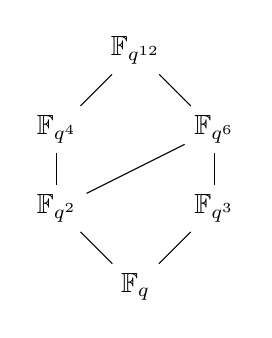
\begin{tikzpicture}
    \node (1) at (0,0) {$\mathbb{F}_{q}$}; 
    \node (2) at (-1,1) {$\mathbb{F}_{q^2}$}; 
    \node (3) at (1,1) {$\mathbb{F}_{q^3}$}; 
    \node (4) at (-1,2) {$\mathbb{F}_{q^4}$}; 
    \node (6) at (1,2) {$\mathbb{F}_{q^6}$}; 
    \node (12) at (0,3) {$\mathbb{F}_{q^{12}}$}; 
    \draw (1) -- (2);
    \draw (1) -- (3);
    \draw (2) -- (4);
    \draw (2) -- (6);
    \draw (3) -- (6);
    \draw (6) -- (12);
    \draw (4) -- (12);
  \end{tikzpicture}
  \caption{The subfields of $\mathbb{F}_{12}$. Two fields are linked if one is a
subfield of the other.}
  \label{fig:F12}
\end{figure}
The $\mathbb{F}_q$-automorphisms of the extension $\mathbb{F}_{q^l}$ are given
by the following result.
\begin{prop}
  Let $q=p^m$ be a prime power and $l\in\mathbb{N}$ an integer.
  The group of $\mathbb{F}_q$-automorphisms of $\mathbb{F}_{q^l}$ is a cyclic
  group of order $l$ generated by
  \[
    \sigma : t\mapsto t^q.
  \]  
\end{prop}
Let $u\in\mathbb{F}_{q^l}$, the conjugates of $u$ are the elements
\[
  \sigma(u), \sigma^2(u), \dots, \sigma^{l-1}(u)
\]
and the orbit of $u$ is the set
\[
  \left\{ u, \sigma(u), \dots, \sigma^{l-1} \right\}.
\]
This orbit might have any length $m$ dividing $l$. The orbit of $u$ is of length
$m$ if and only if $u$ is in a subfield $\mathbb{F}_{q^m}$ of
$\mathbb{F}_{q^l}$. We also sometimes write
\[
  u^\sigma = \sigma(u).
\]
Two maps, defined with the conjugates of a given element,
will play a very important role, the \emph{trace} and the \emph{norm}.
\begin{defi}[Trace and norm]
  Let $q$ a prime power and 
  \[
    \mathbb{F}_{q^l}/\mathbb{F}_q
  \]
  an extension of degree $l$, let $G$ be the group of
  $\mathbb{F}_q$-automorphisms of $\mathbb{F}_{q^l}$, and let
  $u\in\mathbb{F}_{q^l}$. Then the \emph{trace} of $u$ is
  \[
    \tr_{\mathbb{F}_{q^l}/\mathbb{F}_q}(u) = \sum_{\sigma\in G}u^\sigma
  \]
  and the \emph{norm} of $u$ is
  \[
    N_{\mathbb{F}_{q^l}/\mathbb{F}_q}(u)=\prod_{\sigma\in G}u^\sigma.
  \]
\end{defi}
We may only write $\tr$ or $N$ when the extension considered is clear from the
context. The trace over the field $\mathbb{F}_{q}$ is a $\mathbb{F}_{q}$-linear
map, and the norm is a multiplicative map, they are also both \emph{transitive},
as described in the next proposition.
\begin{prop}
  Let $q\in\mathbb{N}$ a prime power and $a\,|\,b\,|\,c$ three integers, giving
  the tower of extensions that follows.
  \begin{center}
  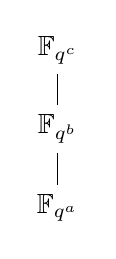
\begin{tikzpicture}
    \node (a) at (0,0) {$\mathbb{F}_{q^a}$}; 
    \node (b) at (0,1) {$\mathbb{F}_{q^b}$}; 
    \node (c) at (0,2) {$\mathbb{F}_{q^c}$}; 
    \draw (a) -- (b);
    \draw (b) -- (c);
  \end{tikzpicture}
  \end{center}
  Let $u\in\mathbb{F}_{q^c}$, then
  \[
    \tr_{\mathbb{F}_{q^c}/\mathbb{F}_{q^a}}(u) =
    \tr_{\mathbb{F}_{q^b}/\mathbb{F}_{q^a}}(\tr_{\mathbb{F}_{q^c}/\mathbb{F}_{q^b}}(u))
  \]
  and
  \[
    N_{\mathbb{F}_{q^c}/\mathbb{F}_{q^a}}(u) =
    N_{\mathbb{F}_{q^b}/\mathbb{F}_{q^a}}(N_{\mathbb{F}_{q^c}/\mathbb{F}_{q^b}}(u)).
  \]
\end{prop}
Finally, the map
\[
  (x, y)\mapsto\tr(xy)
\]
is a non-degenerate bilinear map that we will also sometimes write as
\[
  \ps{x}{y} = \tr(xy).
\]
%
%\subsection{Kummer extensions}
%
%Kummer extensions are a particular kind of extension, they play a special role in
%our construction of lattices of extension presented in
%Chapter~\ref{chap:lattice}. We follow the presentation of~\cite{Lang04}.

\section{Algebraic function fields}
\label{sec:algebraic-function-fields}

% Contents
% ========
%
% - algebraic function field
% - place
% - degree of a place
% - divisor
% - big theorems
% - definition of the genus ?

Together with algebraic curves, algebraic function fields are a way of
describing the algorithms of Chapters~\ref{chap:bilinear}
and~\ref{chap:hypersymmetric}. In this document, we choose to use the algebraic
function field point of view. The function fields we need are constructed
on top of finite fields, so we present the theory with that context in mind. For
this section, our reference is~\cite{Stichtenoth09}. In all the section, $\K$ is
a finite field of characteristic $p$.

\subsection{Places}

Let us first define what an algebraic function field is, together with important
notions leading to the definition of \emph{places}.
\begin{defi}[Algebraic function field]
  An \emph{algebraic function field} $F$ of one variable over $\K$ is an
  extension field 
  \[
    F/\K
  \]
  such that $F$ is a finite algebraic extension of
  $\K(x)$ for some element $x\in F$ which is transcendental over $\K$.
\end{defi}
From now on, the notation $F$ will represent an algebraic function field over
$\K$.
\begin{defi}[Valuation ring]
  A \emph{valuation ring} $\vr$ of the function field $F/\K$ is a ring 
  \[
    \vr \subset F
  \]
  with the following properties
  \begin{enumerate}
    \item $\K\subsetneq\vr\subsetneq F$;
    \item for all $z\in F$, we have $z\in\vr$ or $z^{-1}\in\vr$.
  \end{enumerate}
\end{defi}
Valuation rings $\vr$ are local rings, \ie they have a unique maximal ideal that is
given by 
\[
  P = \vr\setminus\vr^\times
\]
where $\vr^\times$ is the group of units of the ring $\vr$.
\begin{defi}[Place]
  A \emph{place} $P$ of $F$ is the maximal ideal of some valuation ring $\vr$ of $F$.
\end{defi}

% Note
% ====
%
% Maybe a word about the equivalence of the notions of places, discrete valuation
% and valuation ring could be nice here, just a proposition without a proof or
% even a remark not too formal, we'll see.

We let $\mathbb{P}_F$ be the set of places of $F$. If $P\in\mathbb{P}_F$ is a
place of $F$, we denote by $\vr_P$ the corresponding valuation ring. Since $P$
is a maximal ideal of $\vr$, we also know that the quotient ring
\[
  F_P = \vr_P/P
\]
is a field. We call this field $F_P$ the residue class field of $P$.
\begin{defi}[Residue class map]
Let $P\in\mathbb{P}_F$ be a place of $F$. For $x\in F$, we let 
\[
  x(P)
\]
be the residue class of $x$ modulo $P$. If $x\notin P$, we define $x(P)=\infty$.
The map from $F$ to $F_P\cup\left\{ \infty \right\}$
\[
  x\mapsto x(P)
\]
is called the \emph{residue class map}.
\end{defi}
\begin{defi}[Degree of a place]
  Let $P\in\mathbb{P}_F$ a place of $F$. The residue class field $F_P$ is a
  finite extension of $\K$ and we call
  \[
    \deg P = \left[ F_P\,:\,\K \right]
  \]
  the \emph{degree} of $P$.
\end{defi}

\subsection{Divisors}

Now that we now what places are, we can define divisors. In this section, we
keep the notation of last section: we let $F$ be an algebraic function field
over a finite field $\K$ of characteristic $p$.
\begin{defi}[Divisor]
  The \emph{divisor group} $\Div(F)$ of $F$ is defined as the free abelian group generated
  with the places of $F$. The elements of $\Div(F)$ are called the
  \emph{divisors} of $F$. In other words, a divisor is a formal sum
  \[
    D = \sum_{P\in\mathbb{P}_F} n_P\cdot P
  \]
  with $n_P\in\mathbb{Z}$ and $n_P=0$ for all but finitely many places $P$.
  We define the \emph{support} of $D$ as
  \[
    \supp D = \left\{ P\in\mathbb{P}_F\,|\,n_P\neq 0 \right\}.
  \]
\end{defi}


\section{Complexity models}
\label{sec:complexity-models}

When studying algorithms, it is of central interest to understand how our algorithms
\emph{scale}, \ie to understand how they perform if the size of the input is
getting larger and larger. Complexity theory studies this phenomenon and gives us models
of computation in order to quantify the behaviour of our algorithms. Depending
on the situation, not all models are relevant, and one has to balance between
the concreteness of a model and its ease of use. An extreme viewpoint is to
specify an operating system with a compiled programming language and to compare
the running time or the memory requirements between algorithms. The advantage of
such a model is that it is very concrete, but it is also its main disadvantage
because it makes the model hard to use. Thus, there exist other models of
\emph{idealized} computers, such as Turing machines~\cite{Papadimitriou03},
random access machines, or the algebraic complexity model.
We use the latter, that we present in more details in the next section.

\subsection{Algebraic complexity}

This model is widely presented in~\cite{BCS13}, we only give a brief
presentation of the subject. This model assumes that we use an abstract computer
that is able to perform operations in some base field $\K$ at a constant, unit
cost. We also assume that accessing the memory of the computer is free.
Algebraic complexity is especially useful with algorithms dealing with
algebraic structures. This is very handy for us, since
we usually work with algebras
\[
  (\A, +, \times, \cdot)
\]
over some base field $\K$. As an example, with this model, the complexity of an
addition in the extension field
\[
  \mathbb{F}_4 = \mathbb{F}_2[T]/(T^2+T+1) = \mathbb{F}_2(x)
\]
where $x=\bar T$, if elements are represented in the basis $\left\{ 1, x
\right\}$, is $2$, because we only need $2$ additions in $\mathbb{F}_2$ to
perform an addition in $\mathbb{F}_4$. Indeed, if
\[
  a = a_0 + a_1x\in\mathbb{F}_4
\]
and
\[
  b = b_0 + b_1x\in\mathbb{F}_4,
\]
we have
\[
  a+b = (a_0+b_0)+(a_1+b_1)x.
\]
In the case of a multiplication, we have
\[
  ab = (a_0b_0+a_1b_1) + (a_0b_1+a_1b_0)x,
\]
so the complexity of a multiplication in $\mathbb{F}_4$ (at least with this
formula) is $6$, because we need
$4$ multiplications and $2$ additions in $\mathbb{F}_2$. In the context of
finite fields, it makes sense to consider that the cost of an operation is
independent of the operands, because the elements have a fixed size; but this is
no longer the case in other rings, for example in $\mathbb{Z}$, $\mathbb{Q}$,
$\mathbb{R}$, or $\mathbb{C}$. We could also argue that the different operations
in $\K$ should not have the same cost, we thus present an other manner of
computing the complexity of an algorithm, that is called \emph{bilinear
complexity}, in Chapter~\ref{chap:bilinear}.

\subsection{Landau notations}

In order to describe the asymptotic behaviour of an algorithm, we use the
classical \emph{big O} and \emph{little o} notations $O$ and $o$. Let $f:\mathbb{R}\to\mathbb{R}$ and
$g:\mathbb{R}\to\mathbb{R}$ be two functions, we write
\[
  f(x) = O(g(x))
\]
if there exist $M\in\mathbb{R}$ and $C>0$ such that
\[
  \forall x\geq M,\,|f(x)|\leq Cg(x).
\]
and we write
\[
  f(x)=o(g(x))
\]
if there exist $M\in\mathbb{R}$ and $\varepsilon:\mathbb{R}\to\mathbb{R}$, a
function with $\varepsilon(x)\to 0$ when $x\to\infty$, such
that
\[
  \forall x\geq M,\,|f(x)|\leq \varepsilon(x)g(x).
\]
We say that $f$ is equivalent to $g$ and we write
\[
  f(x)\sim g(x)
\]
if 
\[
 f(x)-g(x) = o(g(x))
\]
when $x\to\infty$. Finally, we also use the \emph{soft O} notation $\tilde{O}$ to neglect
logarithmic factors in the big O notation, we write
\[
  f(x) = \tilde{O}(g(x))
\]
if there exist some $k$ with $f(x) = O(g(x)\log^k(g(x)))$.



\chapter{Bilinear complexity and Chudnosky$^2$-type algorithms}
In the \emph{algebraic complexity model}~\cite{BCS13}, we assume that our
machine is able to perform any operation in some base field $\K$ in constant,
unit time. This is an idealized model made in order to simplify the
computation of the complexity of algebraic algorithms. Nevertheless,
multiplication of two variable quantities in $\K$ is arguably more expensive
than addition, or than multiplication of a variable by a fixed constant. In the
context of the computation of bilinear maps, extensive work has been done to
reduce the number of two-variable multiplications involved. Notable examples are
Karatsuba's algorithm~\cite{Karatsuba63} and
Strassen's algorithm~\cite{Strassen69}. Karatsuba's algorithm is
based on the fact that the bilinear map associated to the product of two
polynomials of degree $1$
\[
  A = a_1 X + a_0\text{ and }B = b_1 X + b_0
\]
can be computed with three products
\[
  c_0 = a_0b_0,
\]
\[
  c_1 = (a_0+a_1)(b_0+b_1),
\]
and
\[
  c_\infty = a_1b_1,
\]
instead
of the four classic ones $a_0b_0$, $a_0b_1$, $a_1b_0$ and $a_1b_1$ as follows:
\[
  AB = c_\infty X^2 + (c_1-c_\infty-c_0) X + c_0.
\]
It will become clear in Section~\ref{sec:evalinter} why we use the index
$\infty$ instead of $2$ for $c_\infty = a_1b_1$. Strassen's algorithm
exploits a similar idea in the case of $2\times2$ matrices: only $7$ products
are used instead of $8$ in order to compute a matrix product. Both these
algorithms have very practical consequences. Karatsuba's algorithm is used in
computer algebra softwares, when the standard multiplication is no longer
optimal, and when the Discrete Fourier Transform (DFT) is not yet the fastest.
Strassen's algorithm, used reccursively, is the fastest strategy available for
large matrix multiplication. Both these questions are treated in~\cite{GG13}.
Thus the idea of minimizing the number of multiplications, even if it means
having to compute more additions and substractions, seems a good idea.

The \emph{bilinear complexity}
$\mu(\Phi)$ of a bilinear map $\Phi$ over $\K$ represents the minimum number of two-variable
multiplications in a formula that computes $\Phi$, discarding the cost of other
operations such as addition or multiplication by a constant. In other words, in
this model of computation, we only count $2$-variable multiplications, and other
operations are assumed to have no cost. It is motivated by the fact that
$2$-variable multiplication is often more expensive to compute than other
operations and by the practicality of algorithms minimizing the multiplications,
such as Karatsuba's and Strassen's.
In particular when $\A$ is a finite dimensional algebra over $\K$,
we define the bilinear complexity of $\A$ as $\mu(\A/\K)=\mu(m_{\A})$
where $m_{\A}:\A\times\A\to\A$ is the multiplication map in $\A$ seen
as a $\K$-bilinear map.

Let $\K^{2\times2}$ be the algebra
of $2\times2$ matrices over $\K$. We know thanks to Strassen's algorithm that
\[
  \mu(\K^{2\times 2}/\K) \leq 7.
\]
In fact, this is optimal, so we have exactly $\mu(\K^{2\times2}/\K)=7$. In
general, it seems to be hard to find the bilinear complexity of a given algebra,
for example the bilinear complexity of $\K^{3\times3}$ is not known.
In the litterature, work has been done both to algorithmically find the bilinear complexity of
small algebras~\cite{BDEZ12, Covanov19} and to understand how the bilinear
complexity asymptotically grows~\cite{CC88, BCPRRR19}. Chudnovsky and Chudnovsky
proved in 1988 that the bilinear complexity of an extension field
$\mathbb{F}_{q^k}/\mathbb{F}_{q}$ is linear in the degree $k$ of the
extension, using an evaluation-interpolation method on curves. We present this
technique in the next section.

\section{Evaluation - Interpolation}
\label{sec:evalinter}

Let $P\in\K[x]$ be a polynomial with coefficients in a finite field $\K$. The
evaluation-interpolation strategy is based on two facts:
\begin{itemize}
  \item a polynomial of degree $n$ can be described by its values at $n+1$
    points and reconstructed via \emph{interpolation};
  \item the \emph{evaluation} map at some point $a\in\K$ is a homomorphism of ring from
    $\K[x]$ to $\K$.
\end{itemize}
\paragraph{Interpolation.} The fact that a polynomial $P\in\K[x]$ of degree $n$
is uniquely determined by its values at $n+1$ (different) points in $\K$ follows
from the fact that a polynomial of degree $n$ with coefficients in $\K$ has up
to $n$ roots. This gives us the \emph{uniqueness} of the polynomial. As for the
\emph{existence}, it follows from the Lagrange interpolation. Let $x_1, \dots,
x_{n+1}\in\K$ be $n+1$ points in $\K$ and $y_1, \dots, y_{n+1}$ the
corresponding evaluation values, such that
\[
  \forall j\in\left\{ 1, \dots, n+1 \right\},\,y_j = P(x_j).
\]
Let 
\[
  L_j = \prod_{i\neq j}\frac{x-x_i}{x_j-x_i},
\]
we then have $L_j(x_i) = \delta_{i, j}$ with
\[
  \delta_{i, j} = 
  \left\{\begin{array}{ll}
      1&\mbox{if } i=j\\
      0&\mbox{if } i\neq j
    \end{array}
    \right.
\]
the Kronecker symbol. Now, the polynomial
\[
  P = \sum_{j=1}^{n+1} y_j L_j
\]
meets all the evaluation conditions and is the sum of polynomials of degree $n$
so $P$ is of degree at most $n$.

\paragraph{Evaluation.} Let $P, Q\in\K[x]$ be two polynomials with coefficients
in $\K$ and $a\in\K$, then we have
\[
  (P+_{\K[x]}Q)(a) = P(a) +_{\K} Q(a)
\]
and 
\[
  (P\times_{\K[x]} Q)(a) = P(a) \times_{\K} Q(a),
\]
where $+_{\K[x]}, \times_{\K[x]}$ (resp. $+_{\K}, \times_{\K})$ are the addition
and multiplication operations in $\K[x]$ (resp. $\K$).
In other words, the map
\[
\begin{array}{llll}
  \textrm{ev}_a:&\K[x]&\to&\K\\
  &P&\mapsto&P(a)
\end{array}
\]
is an homomorphism of rings from $\K[x]$ to $\K$.

We are used to represent polynomials by their coefficients, but these two facts
suggest that we can also represent polynomials by their values at some points.
With this representation, adding two polynomials is done by adding the
values, which is done with linear complexity, the same as with the coefficient
representation. But the multiplication of polynomials is also obtained via the
multiplication of the values, which is linear again and better than the
quadratic complexity obtained with the usual multiplication formula for the
coefficients. An important problem is then to be able to change between
representations at a small cost, this is done using well-chosen points of
evaluation and this strategy is known under the name of Fast Fourier
Transform (FFT)~\cite{GG13}. Let $P, Q\in\K[x]$ be two polynomials with
coefficients in $\K$ represented by their coefficients, such that
$\deg(PQ)=n-1$. In order to multiply $P$ and $Q$ we need at least $n$ points in
$\K$ and the evaluation-interpolation strategy consists in $3$ steps:
\begin{enumerate}
  \item multipoint evaluation of $P$ and $Q$ at $n$ points $a_1, \dots, a_n$;
  \item coordinate-wise multiplication;
  \item interpolation to reconstruct the product $PQ$.
\end{enumerate}
When there are not enough points in $\K$ to use this method, instead of
evaluating on points of $\K$, we can evaluate the polynomials on points of
curves on $\K$ with enough points. As a first example, we can interpret
Karatsuba's algorithm as an evaluation-interpolation scheme on
the projective line $\mathbb{P}^1(\K)$. Let 
\[
  P = a_1 x + a_0
\]
and 
\[
  Q = b_1 x + b_0,
\]
then
\[
  c_0 = \textrm{ev}_0(P)\textrm{ev}_0(Q) = a_0b_0
\]
is obtained via evaluation at $0$,
\[
  c_1 = \textrm{ev}_1(P)\textrm{ev}_1(Q) = (a_0+a_1)(b_0+b_1)
\]
is obtained via evaluation at $1$,
\[
  c_\infty = \textrm{ev}_\infty(P)\textrm{ev}_\infty(Q) = a_1b_1
\]
is obtained via evaluation at the point at infinity, where the evaluation at
infinity $\textrm{ev}_{\infty}$ is the function mapping a polynomial to its
leading coefficient. This strategy can be generalized to curves more complex
that $\mathbb{P}^1(\K)$, as was done by Chudnovsky and Chudnovsky in
$1988$~\cite{CC88}.


\section{Complexities}
% Both algorithmic results in small dimension and asymptotic results with
% Chudnosky-like techniques would be better I guess


\chapter{Hypersymmetric bilinear complexity}
In Chapter~\ref{chap:bilinear}, we have seen the notions of bilinear complexity
and symmetric bilinear complexity. We now investigate even stronger
notions of symmetry, allowing to have very short representations of a bilinear
map.

\minitoc

% TODO
% ====
%
% Find a nice picture to put here to illustrate something in link with the
% chapter.

\clearpage
\section{Symmetric and hypersymmetric fomulas}
% Table of content
% ================
%
% - Recall of the definition of symmetric
% - Existence and lemma for the symmetric case
% - non degenerate bilinear form, link with the trace, but not only
% - Link between symmetric and hypersymmetric in smaller dimension
% - Galois invariance
% - Comment for the case of the particular algebras we study, what is known and
%   what is not
%
% Comment
% =======
%
% Comment about the trisymmetric formulas, it is true that F_4/F_2 can be
% represented by a trisymmetric formula but it is not the case for F_8/F_2. We
% should check the lemma saying something on the existence of the trisymmetric
% decomposition, but it is probably just simpler.

Let $\K$ be a finite field, $V_1$, $V_2$ and $W$ three finite-dimensional $\K$-vector
space and
\[
  \Phi:V_1\times V_2\to W
\]
a bilinear map. Recall Definition~\ref{defi:bilinear-formula}:
\[
  \Phi(x, y) = \sum_{j=1}^t\varphi_j(x)\psi_j(y)w_j,
\]
where for all $1\leq j\leq t$, $\varphi_j\in V_1^\vee$ and $\phi_j\in V_2^\vee$ are linear forms and
$w_j\in W$ is a vector, is called a \emph{bilinear formula} of length $t$. If
the spaces $V_1$ and $V_2$ are equal and if the bilinear map $\Phi$ is
symmetric, \ie if for all $x, y\in V$
\[
  \Phi(x, y) = \Phi(y, x),
\]
we can investigate the existence of formulas satisfying the same condition of
symmetry, \ie formulas where for all $1\leq j\leq t$, $\varphi_j=\psi_j$,
resulting in \emph{symmetric} bilinear form:
\[
  \Phi(x, y) = \sum_{j=1}^t\varphi_j(x)\varphi_j(y)w_j.
\]
In fact, we can define other interesting types of symmetries, but it is useful
to first generalize the notions that we saw in Chapter~\ref{chap:bilinear} to
higher dimensions.
\subsection{Generalization to multilinear maps}
The definitions of bilinear formula and bilinear complexity are not bound to the
bilinear case and can be generalized to arbitrary dimension. These general
definitions will be used in Section~\ref{subsec:trisym} to define
\emph{hypersymmetric} complexity.
\begin{defi}[Multilinear formula]
Let $V_1, V_2, \dots, V_s$ and $W$ be $s+1$ finite-dimensional $\K$-vector
spaces and
\[
  \Phi:V_1\times V_2\times\dots\times V_s\to W
\]
an $s$-linear map. A \emph{multilinear formula}, or \emph{multilinear
decomposition}, or \emph{multilinear algorithm} of length $t$ for $\Phi$ is a
collection of $s\times t$ linear forms $\varphi_1^{(1)}, \varphi_2^{(1)}, \dots,
\varphi_t^{(1)}\in V_1^\vee$ up to $\varphi_1^{(s)}, \varphi_2^{(s)}, \dots,
\varphi_t^{(s)}\in V_s^{\vee}$ and $t$ vectors $w_1, \dots, w_t$, such that for all $x_1\in V_1, \dots, x_s\in
V_s$, we have
\[
  \Phi(x_1, \dots, x_s) =
  \sum_{j=1}^t\varphi_j^{(1)}(x_1)\dots\varphi_j^{(s)}(x_s)w_j.
\]
\end{defi}
\begin{defi}[Multilinear complexity]
Let $V_1, V_2, \dots, V_s$ and $W$ be $s+1$ finite-dimensional $\K$-vector
spaces and
\[
  \Phi:V_1\times V_2\times\dots\times V_s\to W
\]
an $s$-linear map. The \emph{multilinear complexity} $\mu(\Phi)$ of $\Phi$ is the
minimal length $t$ of a multilinear formula for $\Phi$.
\end{defi}
As in the case of bilinear complexity, the multilinear complexity $\mu(\Phi)$ of a
multilinear map $\Phi$ can also be defined as the rank of the tensor in 
\[
  V_1^\vee\otimes\dots\otimes V_s^\vee\otimes W
\]
corresponding to $\Phi$, see Example~\ref{ex:bilinear-complexity} for an
illustration of this correspondence in the bilinear case. In the case where
\[
  V_1 = V_2 = \dots = V_s,
\]
symmetric formulas and
symmetric complexity can also be generalized when $\Phi$ is a \emph{symmetric}
multilinear map, \ie when for all permutation $\sigma\in\mathfrak S_s$ and for
all vectors $x_1, \dots, x_s\in V$, we have
\[
  \Phi(x_1, \dots, x_s) = \Phi(\sigma(x_1), \dots, \sigma(x_s)).
\]
\begin{defi}[Symmetric multilinear formula]
Let $V$ and $W$ be two finite-dimensional $\K$-vector
spaces and
\[
  \Phi:\underset{\textrm{$s$ times}}{\underbrace{V\times\dots\times V}}\to W
\]
a symmetric $s$-linear map. A \emph{symmetric multilinear formula}, or
\emph{symmetric multilinear
decomposition}, or \emph{symmetric multilinear algorithm} of length $t$ for $\Phi$ is a
collection of $t$ linear forms $\varphi_1, \varphi_2, \dots,
\varphi_t\in V^\vee$ and $t$ vectors $w_1, \dots, w_t$, such that for all $x_1, \dots, x_s\in
V$, we have
\[
  \Phi(x_1, \dots, x_s) =
  \sum_{j=1}^t\varphi_j(x_1)\dots\varphi_j(x_s)w_j.
\]
\end{defi}
\begin{defi}[Symmetric multilinear complexity]
Let $V$ and $W$ be two finite-dimensional $\K$-vector
spaces and
\[
  \Phi:\underset{\textrm{$s$ times}}{\underbrace{V\times\dots\times V}}\to W
\]
a symmetric $s$-linear map. The \emph{symmetric multilinear complexity} $\musym(\Phi)$ of $\Phi$ is the
minimal length $t$ of a symmetric multilinear formula for $\Phi$. If no such
formula exists, we set
\[
  \musym(\Phi) = \infty.
\]
\end{defi}
Contrary to the bilinear case, some symmetric multilinear maps do not admit a symmetric
decomposition, but the problem of whether a symmetric multilinear map admits
a symmetric multilinear formula is well understood and follows from
Theorem~\ref{thm:symmetric-formula}.
\begin{thm}[{\cite[Thm.~A.7]{Randriam15}}]\label{th:criterion}
\label{thm:symmetric-formula}
Let $\Phi:V^s\to W$ be a $s$-linear map between finite dimensional vector spaces over $\mathbb{F}_q$.
Then $\Phi$ admits a symmetric decomposition if and only if $\Phi$ is \emph{Frobenius-symmetric},
\ie if and only if it is symmetric and one of the following two conditions holds:
\begin{itemize}
\item $s\leq q$
\item $s\geq q+1$ and for all $u,v,z_1,\dots,z_{s-q-1}$ in $V$,
\[
\Phi(\underset{\textrm{$q$ times}}{\underbrace{u,\dots,u}},v,z_1,\dots,z_{s-q-1})=\Phi(u,\underset{\textrm{$q$ times}}{\underbrace{v,\dots,v}},z_1,\dots,z_{s-q-1}).
\]
\end{itemize}
\end{thm}

\subsection{Trisymmetric and hypersymmetric complexity}
\label{subsec:trisym}

Under even stricter conditions, we can study the existence of even more
symmetric formulas. These formulas allow to describe a multilinear map with
fewer elements, and thus give a compact definition of the map. Since the
symmetry conditions are stronger there are fewer such formulas, and as a
consequence the search space is smaller. Thus, we expect algorithms to be
faster, as was the case when using Barbulescu \etal algorithm
(Algorithm~\ref{algo:BDEZ}) to find symmetric formulas. Let us define those
``stricter conditions''. Let
\[
  \Phi:V^s\to V
\]
be an $s$-linear symmetric map, \ie we additionnaly ask that $W=V$. We also
assume that $V$ has a non-degenerate symmetric bilinear form, that we write as a
scalar product
\[
 \begin{array}{ccc}
 V\times V &\to&\K\\
 (v,w)&\mapsto&\ps{v}{w}.
 \end{array}
\]
In that case, we know that the vector space $V$ is isomorphic to its dual space
$V^\vee$:
\[
  V\cong V^\vee,
\]
\ie for each linear form $\varphi\in V^\vee$, there exist a unique vector $a\in
V$ such that for all $x\in V$, we have
\[
  \varphi(x) = \ps{a}{x}.
\]
Under these conditions, we can now write a symmetric formula for $\Phi$ as
\[
  \Phi(x, y) = \sum_{j=1}^t\ps{a_i}{x}\ps{a_i}{y}w_j
\]
where for all $1\leq j\leq t$, $a_j\in V$ is a vector of $V$. As a consequence,
we can also describe a symmetric formula for $\Phi$ as the data of vectors
$(a_j)_{1\leq j\leq t}$ and $(w_j)_{1\leq j\leq t}$. In order to have an even
more compact description of $\Phi$, one can ask for the vectors $w_j$ to be
proportional to $a_i$, leading to the definition of hypersymmetric
formula.
% Note
% ====
%
% But is that really natural? Wouldn't it be better to say that we would like
% the a_i and the b_i to be equal? 
%
% TODO
% ====
%
% Maybe change this to include the case a_i = b_i and discuss it a little, or
% maybe not, we'll see.
%
% Remark
% ======
%
% If this is presented, it could be nice to have the tensor point of view, with
% a decomposition with the same elements three times being then very clear.

\begin{defi}[Hypersymmetric formula]
Let $V$ a finite-dimensional $\K$-vector
spaces equipped with a saclar product and
\[
  \Phi:\underset{\textrm{$s$ times}}{\underbrace{V\times\dots\times V}}\to W
\]
a symmetric $s$-linear map. A \emph{hypersymmetric formula}, or
\emph{hypersymmetric decomposition}, or \emph{hypersymmetric algorithm} of length $t$ for $\Phi$ is a
collection of $t$ vectors $a_1, \dots, a_t\in V$ and $t$ scalars $\lambda_1,
\dots, \lambda_t\in\K$, such that for all $x_1, \dots, x_s\in
V$, we have
\[
  \Phi(x_1, \dots, x_s) =
  \sum_{j=1}^t\lambda_j\ps{a_j}{x_1}\dots\ps{a_j}{x_s}a_j.
\]
\end{defi}
\begin{defi}[Hypersymmetric complexity]
Let $V$ be a finite-dimensional $\K$-vector spaces equipped with a saclar product
and
\[
  \Phi:\underset{\textrm{$s$ times}}{\underbrace{V\times\dots\times V}}\to W
\]
a symmetric $s$-linear map. The \emph{hypersymmetric complexity} $\muhyp(\Phi)$ of $\Phi$ is the
minimal length $t$ of a hypersymmetric formula for $\Phi$. If no such
formula exists, we set
\[
  \muhyp(\Phi) = \infty.
\]
\end{defi}
\begin{ex}
  \label{ex:trisymmetric-formula}
  We take the same case as in Example~\ref{ex:bilinear-complexity}, but viewed
  a bit differently. Let $\K=\mathbb{F}_2$ and 
  \[
    V=\mathbb{F}_4\cong\mathbb{F}_2[T]/(T^2+T+1)\cong\mathbb{F}_2(\zeta)
  \]
  seen as a $\mathbb{F}_2$-vector space of dimension $2$ using the base $(1,
  \zeta)$. The $\mathbb{F}_2$-bilinear map $\Phi$ that we
  consider is the product in $\mathbb{F}_4$:
  \[
 \begin{array}{cccc}
   \Phi: & \mathbb{F}_4\times \mathbb{F}_4 &\to&\mathbb{F}_4\\
 &(x,y)&\mapsto&xy.
 \end{array}
  \]
  We also consider the non-degenerate symmetric bilinear form
\[
 \begin{array}{ccc}
   \mathbb{F}_4\times \mathbb{F}_4 &\to&\mathbb{F}_2\\
 (v,w)&\mapsto&\tr(vw),
 \end{array}
\]
where $\tr$ is the trace of the field extension $\mathbb{F}_4/\mathbb{F}_2$,
and we write
\[
  \tr(xy) = \ps{x}{y}.
\]
If $x = x_0 + x_1\zeta\in\mathbb{F}_4$ is an element in the extension field, we have $\tr(x) = x_1$, and if $y = y_0
+ y_1\zeta\in\mathbb{F}_4$ is another element, then their product is
\[
  xy = x_0y_0 + x_1y_1 + (x_0y_1 + x_1y_0 + x_1y_1)\zeta.
\]
We also see that
\[
\left\{ 
  \begin{array}{lll}
    \ps{1}{x}\ps{1}{y} &=& x_1y_1 \\
    \ps{1+\zeta}{x}\ps{1+\zeta}{y} &=& x_0y_0 \\
    \ps{\zeta}{x}\ps{\zeta}{y} &=& (x_0+x_1)(y_0+y_1)
  \end{array}
\right.
\]
and thus we have
\[
  xy =
  \ps{1}{x}\ps{1}{y}\cdot1+\ps{1+\zeta}{x}\ps{1+\zeta}{y}\cdot(1+\zeta)+\ps{\zeta}{x}\ps{\zeta}{y}\cdot\zeta.
\]
This is an hypersymmetric formula of length $3$, and we can prove that there are
no formulas of length $2$, so we have
\[
  \muhyp(\Phi) = 3.
\]
This is in fact the very same formula as in
Example~\ref{ex:bilinear-complexity}.
\end{ex}
In order to investigate the existence of hypersymmetric decompositions, we
remark that there is a natural link between hypersymmetric decompositions of 
the $s$-linear map
\[
  \Phi:V^s\to V
\]
and symmetric decompositions of the $(s+1)$-linear form $\widetilde\Phi$ defined by
\[
  \begin{array}{llll}
    \widetilde\Phi:&V^{s+1}&\to&\K\\
    &(x_1, \dots, x_{s+1})&\mapsto&\ps{\Phi(x_1, \dots, x_s)}{x_{s+1}}
  \end{array}
\]
in the sense of~Lemma~\ref{lm:link-hyp-sym}. Moreover, we say that the
$s$-linear map $\Phi$ is \emph{hypersymmetric} if the associated $(s+1)$-linear
form $\widetilde\Phi$ is symmetric.
\begin{lm}
  \label{lm:link-hyp-sym}
  Let $V$ a $\K$-vector space and 
  \[
    \Phi:V^s\to V
  \]
  a symmetric $s$-linear map. 
Elements $(a_j)_{1\leq j\leq t}$ in $V$ and scalars $(\lambda_j)_{1\leq j\leq t}$ in $\K$ define a hypersymmetric formula for the $s$-linear map $\Phi$,
\[
\Phi(x_1,\dots,x_s)=\sum_{j=1}^{t}\lambda_j\ps{a_j}{x_1}\cdots\ps{a_j}{x_t}a_j,
\]
if and only if they define a symmetric formula for the $(s+1)$-linear form $\widetilde{\Phi}$,
\[
\widetilde{\Phi}(x_1,\dots,x_s,x_{s+1})=\sum_{j=1}^{t}\lambda_i\ps{a_j}{x_1}\cdots\ps{a_j}{x_t}\ps{a_j}{x_{s+1}}.
\]

Thus, $\Phi$ admits a hypersymmetric formula if and only if $\widetilde{\Phi}$ is Frobenius-symmetric (in the sense of Theorem~\ref{thm:symmetric-formula}),
and we have
\[
\muhyp(\Phi)=\musym\left(\widetilde{\Phi}\right).
\]

In particular, if $q\geq s+1$, then any hypersymmetric $s$-linear map over $\mathbb{F}_q$ admits a hypersymmetric formula.
\end{lm}
\begin{proof}
  Assume that $\Phi$ admits a hypersymmetric decomposition, such that for all
  $x_1, \dots, x_s\in V$, we have
  \[
    \Phi(x_1,\dots,x_s)=\sum_{j=1}^{t}\lambda_i\ps{a_j}{x_1}\cdots\ps{a_j}{x_t}a_j,
  \]
  then, by taking the scalar product with any $x_{s+1}$, we obtain
\[
  \ps{\Phi(x_1, \dots,
  x_s)}{x_{s+1}}=\widetilde{\Phi}(x_1,\dots,x_s,x_{s+1})=\sum_{j=1}^{t}\lambda_i\ps{a_j}{x_1}\cdots\ps{a_j}{x_t}\ps{a_j}{x_{s+1}},
\]
which defines a symmetric decomposition for $\widetilde\Phi$. In the other
direction, assume that $\widetilde\Phi$ admits a symmetric decomposition, such
that for all $x_1, \dots, x_{s+1}\in V$, we have
\[
\widetilde{\Phi}(x_1,\dots,x_s,x_{s+1})=\sum_{j=1}^{t}\lambda_i\ps{a_j}{x_1}\cdots\ps{a_j}{x_t}\ps{a_j}{x_{s+1}}.
\]
It can also be written as
\[
  \ps{\Phi(x_1, \dots,
  x_s)}{x_{s+1}}=\ps{\sum_{j=1}^t\lambda_j\ps{a_j}{x_1}\cdots\ps{a_j}{x_s}a_j}{x_{s+1}},
\]
so that we have
\[
  \ps{\Phi(x_1, \dots,
  x_s)-\sum_{j=1}^t\lambda_j\ps{a_j}{x_1}\cdots\ps{a_j}{x_s}}{x_{s+1}}=0.
\]
Since the scalar product $\ps{\cdot}{\cdot}$ is non-degenerate, it means that
  \[
    \Phi(x_1,\dots,x_s)=\sum_{j=1}^{t}\lambda_i\ps{a_j}{x_1}\cdots\ps{a_j}{x_t}a_j.
  \]
  Hence $\Phi$ admits a hypersymmetric decomposition. The other assertions
  follow.
\end{proof}
The most important case is arguably the bilinear case, where $s=2$, because it
was thoroughly studied. For that reason, we sometimes replace the word
hypersymmetric by \emph{trisymmetric} in that particular case, because of the
form of the formulas
\[
  \Phi(x, y) = \sum_{j=1}^t\lambda_j\ps{a_j}{x}\ps{a_j}{y}a_j
\]
that includes the same element $a_j$ three times, and we write $\mutri(\Phi)$
instead of $\muhyp(\Phi)$. Lemma~\ref{lm:link-hyp-sym} states that, if $q\geq3$, a
trisymmetric map $\Phi$ always admits a trisymmetric decomposition.

\subsection{Galois invariance}

An other type of interesting decompositions is Galois invariant decompositions.
It is motivated by the study of group actions on the set of decompositions, that
can sometimes be used to cut branches in the search tree of the algorithms.
% TODO
% ====
%
% Link that with BDEZ stab, the version using automorphisms, and Covanov.
Let 
\[
 \begin{array}{cccc}
   \sigma: & V\times V &\to&V\\
 &x&\mapsto&x^\sigma
 \end{array}
\]
be a $\K$-automorphism of $V$ that respects the scalar product, \ie for all $x,
y\in V$, we have
\[
  \ps{x^\sigma}{y^\sigma} = \ps{x}{y}.
\]
Then, if $\sigma$ is also compatible with some studied multilinear map $\Phi$, it induces
an action on the set of decomposition, as explained in
Lemma~\ref{lm:action-sym}.
\begin{lm}
  \label{lm:action-sym}
  Let $V$ a finite-dimensional $\K$-vector space and
  \[
    \Phi:V^s\to V
  \]
  a symmetric $s$-linear map that is compatible with $\sigma$, \ie for all $x_1,
  \dots, x_s$ in $V$, we have
  \[
    \Phi(x_1^\sigma, \dots, x_s^\sigma) = \Phi(x_1, \dots, x_s)^\sigma.
  \]
  If $(a_j)_{1\leq j \leq t}$ and $(b_j)_{1\leq j \leq t}$ define a symmetric
  formula for $\Phi$
  \[
    \Phi(x_1, \dots, x_s) = \sum_{j=1}^t\ps{a_j}{x_1}\dots\ps{a_j}{x_s}b_j,
  \]
  then $(a_j^\sigma)_{1\leq j\leq t}$ and $(b_{j}^\sigma)_{1\leq j\leq t})$ also
  define a symmetric formula for $\Phi$
  \[
    \Phi(x_1, \dots, x_s) =
    \sum_{j=1}^t\ps{a_j^\sigma}{x_1}\dots\ps{a_j^\sigma}{x_s}b_j^\sigma.
  \]
\end{lm}
\begin{proof}
 Assume that we have a symmetric decomposition for $\Phi$, with the same
 notations as in the Lemma. First, notice that for every $x,y\in V$, we have
 \[
   \ps{x^\sigma}{y} = \langle{x},{y^{\sigma^{-1}}}\rangle.
 \]
 Then, it follows that
 \begin{align*}
   \Phi(x_1, \dots, x_s) &= \Phi(x_1^{\sigma^{-1}}, \dots,
   x_{s}^{\sigma^{-1}})^\sigma\\
   &=
   (\sum_{j=1}^t\langle{a_j},{x_1^{\sigma^{-1}}}\rangle\dots\langle{a_j},{x_s^{\sigma^{-1}}}\rangle
   b_j)^\sigma\\
   &= \sum_{j=1}^t\ps{a_j^{\sigma}}{x_1}\dots\ps{a_j^\sigma}{x_s}b_j^\sigma.
 \end{align*}
 Thus we have a new symmetric formula for $\Phi$.
\end{proof}
When this action, does not change the formula, we then say that it is
$\sigma$-invariant.
\begin{defi}[$\sigma$-invariance]
  Let $(a_j)_{1\leq j\leq t}$ and
$(b_j)_{1\leq j\leq t}$ define a symmetric formula for $\Phi$
  \[
    \Phi(x_1, \dots, x_s) = \sum_{j=1}^t\ps{a_j}{x_1}\dots\ps{a_j}{x_s}b_j.
  \]
We say that this
formula is $\sigma$-invariant if it is the same as the formula defined by
$(a_j^\sigma)_{1\leq j\leq t}$ and $(b_j^\sigma)_{1\leq j\leq t}$,
\ie if there is a permutation $\pi\in\mathfrak S_t$ of $\{1,\dots,t\}$ such that
$(a_j^\sigma,b_j^\sigma)=(a_{\pi(j)},b_{\pi(j)})$ for all $j$. This also applies
to hypersymmetric formulas, setting $b_j=\lambda_j a_j$. 
\end{defi}
\begin{ex}
  In fact, the trisymmetric formula seen in
  Example~\ref{ex:trisymmetric-formula} was already $\sigma$-invariant. Recall
  that we work in $\mathbb{F}_4$, defined by
  \[
   \mathbb{F}_4\cong\mathbb{F}_2[T]/(T^2+T+1)\cong\mathbb{F}_2(\zeta),
  \]
  and we take
\[
  \tr(xy) = \ps{x}{y}.
\]
The $\mathbb{F}_2$-automorphism that we consider is the Frobenius automorphism
\[
  \begin{array}{cccc}
    \sigma: & \mathbb{F}_4 & \to & \mathbb{F}_4 \\
    & x & \mapsto & x^2.
  \end{array}
\]
We still have, for all $x, y\in\mathbb{F}_4$
\[
  xy =
  \ps{1}{x}\ps{1}{y}\cdot1+\ps{1+\zeta}{x}\ps{1+\zeta}{y}\cdot(1+\zeta)+\ps{\zeta}{x}\ps{\zeta}{y}\cdot\zeta.
\]
Since
\[
\left\{ 
  \begin{array}{lll}
    1^\sigma = 1 \\
    \zeta^\sigma=\zeta+1\\
    (\zeta+1)^\sigma=\zeta
  \end{array}
\right.
\]
we wee that the formula is $\sigma$-invariant.
\end{ex}

\subsection{Multiplication formulas in algebras}

In the previous pages, we have defined (hyper)symmetric formulas for any
multilinear map defined over some finite-dimensional $\K$-vector space.
Nevertheless, as seen in the examples, we are often interested in special
instances of multilinear maps. In fact, the map that we have in mind is almost
always the $s$-variable product of some $\K$-algebra $\A$, with $s=2$. There are
two types of algebras we are particularly interested in:
\begin{itemize}
  \item the finite field extensions $\A=\mathbb{F}_{q^m}$, in which we take the
    trace bilinear form
    \[
      \ps{x}{y}=\tr(xy)
    \]
    for our scalar product, and the Frobenius automorphism
    \[
  \begin{array}{cccc}
    \sigma: & \mathbb{F}_{q^m} & \to & \mathbb{F}_{q^m} \\
    & x & \mapsto & x^q.
  \end{array}
\]
for our $\K$-automorphism ;
\item algebras of truncated polynomials $\A = \mathbb{F}_q[T]/(T^m)$. In this
  case, we let 
  \[
  \begin{array}{cccc}
    \tau: & \A & \to & \K \\
    & \sum_{j=0}^{m-1}x_j T^j & \mapsto & x_0
  \end{array}
\]
and
\[
  \ps{x}{y} = \tau(xy).
\]
Indeed, if $x=\sum_{j=0}^{m-1}T^j$ and $y=\sum_{j=0}^{m-1}y_jT^j$, we have
\[
  \tau(x, y) = x_0y_{m-1} + x_1y_{m-2} + \dots + x_{m-1}y_0,
\]
thus $\tau$ is a non-degenerate bilinear form.
\end{itemize}
We denote by $\mutri_q(k)$ the trisymmetric bilinear complexity of the
$2$-variable product in $\mathbb{F}_{q^k}$ and by $\hmutri_q(k)$ the
trisymmetric bilinear complexity of the $2$-variable product in
$\mathbb{F}_q[T]/(T^k)$.

\section{Algorithmic search in small dimension}

In very small dimension, \eg in Examples~\ref{ex:bilinear-complexity}
and~\ref{ex:trisymmetric-formula} where we are working with $\K$-vector spaces
of dimension $2$, the search of formulas can be done by hand relatively easily
because the length of the formulas is short. Though, even in small dimension, if
the cardinality of $\K$ is large, the number of different formulas can be
big, thus making it hard to list \emph{all} different solutions. For these
reasons, it is highly desirable to \emph{algorithmically} find the formulas.
Let $V$ be a finite dimensional $\K$-vector space and $\Phi:V\times V\to V$ a bilinear map.
When wanting to list all the symmetric formulas of the form
\[
  \Phi(x, y) = \sum_{j=0}^t\varphi_j(x)\varphi_j(y)a_j,
\]
Barbulescu~\etal\!\!\!'s and Covanov's algorithms exhaustively search through
all linear forms $\varphi$, cleverly eliminating useless branches in the search
tree. Nevertheless, their methods exploit the fact that it is possible to freely
choose the vectors $a_j\in V$, independently of the linear forms $\varphi_j\in
V^\vee$. This is
no longer possible when searching for trisymmetric decompositions
\[
  \Phi(x, y) = \sum_{j=0}^t\lambda_j\ps{a_j}{x}\ps{a_j}{y}a_j,
\]
because each
linear form $\varphi\in V^\vee$ is linked with a unique vector $a\in V$ such
that for all $x\in V$
\[
  \varphi(x) = \ps{a}{x},
\]
and the choice of a linear form $\varphi_j$ with $\varphi_j(x)=\ps{a_j}{x}$
imposes the choice of the vector $a_j\in V$. We thus propose an \emph{ad hoc}
algorithm to find trisymmetric formulas, exploiting the vector space structure.

% TODO
% ====
%
% Explain in *details* the algorithms, the different ideas to represent the
% bilinear forms, the margins, the fact that some elements can be forgotten
% without them, the way it is implemented in Julia, etc
%
% Note
% ====
%
% Maybe begin with the general framework/idea, like in the WAIFI paper, and
% continue with the different possibilites for the implementation later

\subsection{General algorithm description}

In all the section, we assume that $\K=\mathbb{F}_q$ is the finite field with
$q$ elements, $V$ is a finite-dimensional $\K$-vector space equipped with a
non-degenerate bilinear form, written as a sclar product $\ps{\cdot}{\cdot}$,
and $\Phi:V\times V\to V$ is a hypersymmetric bilinear map for which we want to
compute trisymmetric decompositions
\[
  \Phi(x, y) = \sum_{j=1}^t\lambda_j\ps{a_j}{x}\ps{a_j}{y}a_j.
\]
Assume that
\[
  V\cong\K^m
\]
is a $\K$-vector space of dimension $m$, for which a basis has been chosen and
allows us to identify $V$ to $\K^m$, and
let $(b_j)_{1\leq j\leq m}$ be the bilinear forms on each coordinates, \ie for
all $x,y\in V$, we have
\[
  \Phi(x, y) = (b_1(x, y), \dots, b_m(x, y)).
\]
We have already seen that the difficulty in the trisymmetric case resides in the
fact that each linear form, or equivalently each symmetric rank $1$ bilinear
form, comes with a given vector in $V$ that dictates its impact on the different
coordinates in a trisymmetric formula. Therefore, a central idea is to
exhaustively search through vectors in $V$ instead of linear forms in $V^\vee$.
This is equivalent since 
\[
  V\cong V^\vee
\]
in this case anyway. Moreover, we search through special sets of vectors that
have easy-to-manage coordinates, \eg well-placed zeros and ones, in order to
control the impact on certain coordinates. Assume $(a_j)_{1\leq j \leq t}$ in $V$ and
$(\lambda_j)_{1\leq j \leq t}$ in $\K$ define a trisymmetric decomposition
\[
  \Phi(x, y) = \sum_{j=1}^t\lambda_j\ps{a_j}{x}\ps{a_j}{y}a_j.
\]
Without loss of generality, we can consider that every element $a_j$ is
``normalized'', \ie its first nonzero coordinate is $1$. Indeed, if we have one
\[
  a_{j_0} = 0
\]
for some $1\leq j_0 \leq t$, then we just remove one term from the formula and
we still have a trisymmetric decomposition, of length $t-1$. Now if for every
$1\leq j\leq t$, 
\[
  a_j\neq0,
\]
we let $x_j$ be the first nonzero coordinate of $a_j$ and we write
\[
  a_j = x_j \widetilde a_j.
\]
We can now write the trisymmetric formula as
\begin{align*}
  \Phi(x, y) &= \sum_{j=1}^t\lambda_j\ps{a_j}{x}\ps{a_j}{y}a_j \\
  &= \sum_{j=1}^t\lambda_j\ps{x_j\widetilde a_j}{x}\ps{x_j\widetilde
  a_j}{y}x_j\widetilde a_j \\
  &= \sum_{j=1}^t\lambda_jx_j^3\ps{\widetilde a_j}{x}\ps{\widetilde
  a_j}{y}\widetilde a_j \\
  &= \sum_{j=1}^t\widetilde \lambda_j\ps{\widetilde a_j}{x}\ps{\widetilde
  a_j}{y}\widetilde a_j,
\end{align*}
where $\widetilde\lambda_j = \lambda_jx_j^3$.
Therefore any trisymmetric formula is equivalent to a trisymmetric formula with
normalized vectors, and thus we only search for formulas with normalized
elements. In other words, for all $1\leq j\leq m$, we let
\[
  \E_j=\left\{ x=(x_1, \dots, x_k)\in V
  \,|\, \forall i\leq j-1,\,x_i=0\text{ and }x_j=1 \right\}
\]
and
\[
  \E = \bigcup_{j=1}^m\E_j,
\]
and we search for elements $a_j$ in $\E$ instead of the entire vector space $V$.
Limiting the search to $\E$ helps us in two different ways. First, it reduces
the complexity of the exhaustive search since the cardinality of $\E$ is smaller
than the cardinality of $V$. Indeed, the sets $\E_j$ are disjoint, so
\begin{align*}
  \Card\E &= \sum_{j=1}^m\Card\E_j\\
  &= \sum_{j=1}^m q^{m-j}\\
  &= \cfrac{q^m-1}{q-1},
\end{align*}
whereas
\[
  \Card V = q^m.
\]
Second, it allows a better understanding of what happens in the algorithm,
because if we have some vector
\[
  a\in\E_j
\]
for a given $1\leq j\leq m$, we know that the associated bilinear form
\[
  (x, y)\mapsto\ps{a}{x}\ps{a}{y}
\]
can only impact the coordinates $i\geq j$. Thus, we further
use the vector space structure of $V$ by searching for solutions
on each coordinate, starting with the first coordinates and vectors in $\E_1$,
then the second coordinate and vectors in $\E_2$, and so on until the last
coordinate. Let us focus on the first coordinate first and give some details.

Recall that the goal is to obtain a trisymmetric decomposition for the
hypersymmetric bilinear map $\Phi:V\times V\to V$, that is written
\[
  \Phi(x, y) = (b_1(x, y), \dots, b_m(x, y)).
\]
in the basis of $V$. We first see how to decompose the bilinear \emph{form}
$b_1$ as a sum of rank $1$ bilinear forms. Let $\B$ be the set of bilinear forms
of $V\times V$, recall that $\B$ is a $\K$-vector space of dimension $m^2$, and
that we identify $b_1$ with the $m\times m$ matrix $B_1\in\K^{m\times m}$ 
such that for all vectors $x, y\in V$, we have
\[
  b_1(x, y) = X B_1 Y^t,
\]
where $X, Y\in\K^{1\times m}$ are the row vectors representing $x$ and $y$ and
where $Y^t$ is the transposed of $y$. Let $r_1$ be the rank of $b_1$, we know
that $b_1$ can be decomposed as a sum of $r_1$ bilinear forms of rank $1$. Let
$f$ be the application mapping an element in $V$ to its associated bilinear
form:
\[
  \begin{array}{cccc}
    f: & V & \to & \B\\
    & a & \mapsto & (x, y)\mapsto\ps{a}{x}\ps{a}{y}.
  \end{array}
\]
In order to find the decompositions of $b_1$ as a sum of $r_1$ bilinear forms of
rank $1$, we exhaustively search through scalars $\lambda_1\in\K$ and vectors
$a_1\in \E_1$ such that
\[
  r_1-1=\rank(b_1-\lambda_1 f(a_1)) < \rank(b_1)=r_1,
\]
then, for each such couple $(\lambda_1, a_1)$, we exhaustively search through
scalars $\lambda_2\in\K$ and vectors $a_2\in \E_1$ such that
\[
  r_1-2=\rank(b_1-\lambda_1 f(a_1)-\lambda_2f(a_2)) < \rank(b_1-\lambda_1
  f(a_1))=r_1-1.
\]
We continue this process until we have $r_1$ couples $(\lambda_1, a_1), \dots,
(\lambda_{r_1}, a_{r_1})$ such that
\[
  0 = \rank(b_1-\sum_{j=1}^{r_1}\lambda_jf(a_j)) <
  \rank(\sum_{j=1}^{r_1-1}\lambda_jf(a_j)) = 1,
\]
that exactly means that
\[
  b_1 = \sum_{j=1}^{r_1}\lambda_jf(a_j).
\]
\begin{algorithm}
  \caption{(Minimal decomposition)}
  \label{algo:mindecomp}
  \begin{algorithmic}[1]
    \Require{$b\in \B$ a bilinear form of rank $r$, $E\subset\E$
    the space of vectors in which to search}
    \Ensure{A list of decompositions of $b$ as a sum of bilinear forms of rank
    $1$, each decomposition represented by a set of $r$ couples $\left\{
      (\lambda_1, a_1), \dots, (\lambda_{r}, a_{r})\right\}$.}

    \Procedure{MinimalDecomposition}{$b, E, R_{\text{glob}},
    R_{\text{loc}}=\emptyset$}
    \If{$\varphi=0$}\Comment{$\rank(\varphi)=0$}
    \State $R_\text{glob}\gets R_\text{glob}\bigcup\left\{R_\text{loc}\right\}$
    \Else
    \State $\mathcal C\gets\emptyset$
    \ForAll{$a\in E$}
    \ForAll{$\lambda\in\K$}
  \If{$\rank(b-\lambda f(a))<\rank(b)$}
    \State $\mathcal C\gets\mathcal C\bigcup\left\{ (\lambda, a) \right\}$
    \State \textbf{break}
    \EndIf
    \EndFor
    \EndFor
    \For{$i=1$ to $\Card\mathcal C$}\Comment{$\mathcal
      C=\left\{ (\lambda_1, a_1), \dots, (\lambda_u, a_u) \right\}$}
      \State $E'\gets\left\{ a_{i+1}, \dots, a_u \right\}$
    \State \Call{FindDecMat}{$b-\lambda_i\f(a_i), E', R_\text{glob},
    R_\text{loc}\cup\left\{ (\lambda_i, a_i) \right\}$}
    \EndFor
    \EndIf
    \EndProcedure

   \State $\mathcal R\gets\emptyset$
    \State \Call{MinimalDecomposition}{$b, E, \mathcal R$}
    \State \Return $\mathcal R$
  \end{algorithmic}
\end{algorithm}

% TODO
% ====
%
% Am example of the coordinate search algorithm that is illuminating: probably
% the example of F_{3^3} because it shows the effect of the margins and the
% number of decompositions is only 4. Also a tree showing that the rank
% decreasing technique allows to eliminate some elements in the search would be
% very nice. Maybe there is someting interesting with F_{5^2}, F_{7^2} also?
% F_{11^2} is already less interesting than F_{3^3} I think.

\subsection{Implementation}
\section{Asymptotic complexities}


\part{Efficient arithmetic in a lattice of finite fields}

\chapter{Isomorphism algorithms}
We studied in Part~\ref{part:single} the arithmetic of a single finite field
extension. We now study a set of several extensions. The very first step will be
to understand how to compute an isomorphism (or an embedding) between two finite
fields: that is the material of this chapter.
\minitoc

% TODO: figure

\clearpage

Our reference for this chapter is~\cite{BDDFS17}: we cover a subpart of the
paper because we are interested in the naive isomorphism algorithm (used in
Chapter~\ref{chap:lattice}) and Allombert's algorithm (used in
Chapter~\ref{chap:standard}). We thus do not cover all the isomorphism
algorithms, the reader interested in Rains' algorithm and its elliptic variant
can take a look at the paper cited above.

\section{Generalities and naive algorithm}

Even if our real goal is to compute \emph{embeddings} of finite fields, \ie
ring homomorphisms
\[
  \phi:K\to L
\]
with $K$ and $L$ finite fields, we often refer to the algorithms as
\emph{isomorphism} algorithms. Indeed, computing the embedding $\phi$ is
the same as computing an isomorphism
\[
  \phi':K\to K'
\]
where $K\cong K'$ is isomorphic to a subfield $K'\subset L$ of $L$. The
isomorphism $\phi'$ is just the embedding $\phi$ with its codomain being
restricted to $K'$.

\subsection{Description of the problem}

We let $p$ be a prime number, $\K = \mathbb{F}_p$ be the field with $p$ elements,
and $f, g\in\K[X]$ two irreducible polynomials with
\[
  m=\deg f\mid\deg g=n.
\]
Let
\[
  K=\K[X]/(f(X))\cong\mathbb{F}_{p^m}
\]
and
\[
  L = \K[Y]/(g(Y))\cong\mathbb{F}_{p^n}
\]
two extensions of $\K$. We know there is an embedding
\[
  \phi:K\to L,
\]
unique up to $\K$-automorphism of $K$, \ie there are
\[
  \Card\Gal(K/\K)=m
\]
different embeddings from $K$ to $L$, than can be described as
\[
  \phi\circ\sigma
\]
for $\sigma\in\Gal(K/\K)$. Equivalently, they can also be described as
\[
  \sigma'\circ\phi
\]
with $\sigma'\in\Gal(\phi(K)/\K)$. The \emph{embedding problem} is then to
efficiently find, represent and evaluate one such embedding $\phi$. The problem
is split in two sub-parts.
\begin{description}
  \item[Embedding description problem.] Compute elements $\alpha\in K$ and
    $\beta\in L$ such that 
    \[
      K=\K(\alpha)
    \]
    and such that there exists an embedding $\phi$ mapping $\alpha$ to $\beta$.
  \item[Embedding evaluation problem.] Given elements $\alpha$ and $\beta$
    defined above, and elements $\gamma\in K$, $\delta\in L$, solve the
    following problems:
    \begin{itemize}
      \item compute $\phi(\gamma)\in L$;
      \item test if $\delta\in\phi(K)$;
      \item if $\delta\in\phi(K)$, then compute $\phi^{-1}(\delta)\in K$.
    \end{itemize}
\end{description}
As the name suggests, the \emph{embedding description problem} focuses on
finding a pair of elements that are sufficient to describe an embedding. Indeed,
if 
\[
  K=\K(\alpha)
\]
we know that every element $x\in K$ can be uniquely written as 
\[
  x = \sum_{j=0}^{m-1}a_j\alpha^j
\]
with $a_j\in\K$ for al $0\leq j\leq m-1$, and the embedding $\phi$ is then
defined by
\[
  \phi(x) = \sum_{j=0}^{m-1}a_j\beta^j.
\]
\begin{prop}
  \label{prop:description}
 The elements $\alpha$ and $\beta$
 describe an embedding if and only if they have the same minimal polynomial. 
\end{prop}
\begin{proof}
  Let $\phi:K\to L$ be an embedding mapping $\alpha$ to $\beta$ and let 
  \[
    P = \Minpoly_\K(\alpha)
  \]
  be the the minimal polynomial of $\alpha$. Then 
  \begin{align*}
    P(\beta) &= P(\phi(\alpha)) \\
    &= \phi(P(\alpha))\\
    &= \phi(0) \\
    &= 0
  \end{align*}
  thus $\Minpoly_\K(\beta)\neq 1$ divides $P$ which is irreducible so 
  \[
\Minpoly_\K(\beta) = P.
  \]
 Conversely, if $\alpha$ and $\beta$ have the same minimal polynomial $P$, then the
 map $\phi$ is well-defined and defines an isomorphism between the fields $\K(\alpha)$ and
 $\K(\beta)$, that are both isomorphic to the field
 \[
   \K[X]/(P(X)).
 \]
\end{proof}
While the first problem focuses on finding a description of $\phi$, the
\emph{embedding evaluation problem} independently asks how to efficiently use
the description to compute the actual embedding. We target this question in
Section~\ref{sec:evaluation}.

\subsection{Embedding description problem and naive algorithm}

Until the end of this section and in Section~\ref{sec:allombert}, we deal with
the \emph{embedding description problem}, although we only review a subpart of
the existing algorithms (see~\cite{BDDFS17} for other algorithms). As above, let
$f$ and $g$ two irreducible polynomials with coefficients in $\K$ such that
\[
  m=\deg f\mid \deg g=n.
\]
and let
\[
  K=\K[X]/(f(X))\cong\mathbb{F}_{p^m}
\]
and
\[
  L = \K[Y]/(g(Y))\cong\mathbb{F}_{p^n}
\]
two finite fields. Then one can simply take $\alpha$ to be the class of $X$ in
$K$ and choose $\beta$ to be any root of $f$ in $L$. Indeed, we know that there
is an isomorphic copy of $K$ in $L$ and thus that $f$ splits over $L$.
Furthermore, any root of $f$ will have $f$ as its minimal polynomial, which is
also the minimal polynomial of $\alpha$ by construction. By
Proposition~\ref{prop:description}, the map 
\[
  \phi:K\to L
\]
sending $\alpha$ to $\beta$ is an embedding. The critical routine in that
algorithm is to find a root of $f$ in $L$, that can be done using Shoup-Kaltofen
\emph{equal degree factorization} algorithm~\cite{KS97}. The complexity analysis
of~\cite{BDDFS17} indicates that the cost is strictly larger than quasi-quadratic
complexity $\tilde O(m^2)$. A more efficient algorithm, due to Lenstra and
Allombert, is discussed in Section~\ref{sec:allombert}.

\section{Lenstra-Allombert algorithm}
\label{sec:allombert}

Both Lenstra~\cite{Lenstra91} and Allombert used
Kummer theory, the study of certain field extensions, to compute isomorphisms
between finite fields. But while Lenstra's focus
was on proving the existence of a deterministic isomorphism algorithm, Allombert 
wanted to provide a practical algorithm. This led to the invention of the
Lenstra-Allombert algorithm~\cite{Allombert02} in 2002, for which we give a
description in this section. The ideas of Allombert play an important part in
Chapter~\ref{chap:standard} too. The techniques based on Kummer theories work
for extensions of degree $n$ coprime to the characteristic $p$. In order to have
an algorithm working for any type of extension, the solution is to deal with the
part of the extension which degree is divisible by $p$ separately using
Artin-Shreier theory and to glue the results together in the end.

% TODO
% ====
%
% Add a part on Artin-Shreier?


\subsection{Preliminaries}
\label{sec:preliminaries}

Let us first discuss a simpler case than the general one, that will highlight
the method behind Lenstra-Allombert isomorphism algorithm. Let $K$ and $L$ be
two finite fields of cardinality $p^n$, such that
\[
  K\cong L\cong \mathbb{F}_{p^n}.
\]
Assume that $\gcd(p, n)=1$ and that
\[
  n\mid p-1,
\]
or equivalently that there is a primitive $n$-th root of unity in
$\K=\mathbb{F}_p$, that we denote by $\zeta$. The algorithm is based on
Proposition~\ref{prop:h90}.

\begin{prop}[Hilbert $90$ theorem]
  \label{prop:h90}
  Let $K$ be a finite extension of $\K=\mathbb{F}_p$ of degree $n$ such that there exists a
primitive $n$-th root of unity $\zeta\in\K$ in the base field $\K$, \ie such
that $n$ divides $p-1$. 
 Let $\sigma$ be the generator of the Galois group of the extension
 \[
   K/\K
 \]
 and consider the following equation in $K$.
 \begin{equation}
   \tag{H90}
   \sigma(x) = \zeta x
   \label{eq:h90}
 \end{equation}
The solutions of~\eqref{eq:h90} form a one dimensional $\K$-vector space and if
$\alpha\in K$ is such a solution, we have
\[
  \alpha^n\in\K.
\]
If $\alpha$ is also nonzero, then it is a generator of $K$ over $\K$.
\end{prop}
\begin{proof}
  Let us first construct a nonzero solution of~\eqref{eq:h90}. Consider the polynomial
  \[
    P = \sum_{j=0}^{n-1}\zeta^{-j} X^{p^j}
  \]
  of degree $p^{n-1}$. The polynomial $P$ has at most $p^{n-1}$ roots in $K$,
  which has cardinality $p^n$, so there exists some element $x\in K$ such that
  \[
    y = P(x)\neq0.
  \]
  Now, by construction, we have
  \begin{align*}
    \sigma(y) &= \sigma(\sum_{j=0}^{n-1}\zeta^{-j}x^{\sigma^{j}})\\
    &= \sum_{j=0}^{n-1}\zeta^{-j}x^{\sigma^{j+1}}\\
    &= \zeta \times \sum_{j=0}^{n-1}\zeta^{-(j+1)}x^{\sigma^{j+1}}\\
    &= \zeta \times \sum_{j=1}^{n}\zeta^{-j}x^{\sigma^{j}}\\
    &= \zeta y
  \end{align*}
  and thus $y$ is a nonzero solution of~\eqref{eq:h90}. All the elements
  \[
    \lambda y
  \]
  with $\lambda\in\K$ are also solution of~\eqref{eq:h90} since
  \[
    \sigma(\lambda y) = \lambda\sigma(y) = \zeta\lambda y,
  \]
  and the equation has at most $p$ solutions because the polynomial
  \[
    X^p - \zeta X
  \]
  has at most $p$ roots in $K$. Thus there are exactly $p$ different solutions,
  that are the elements of $\Vect(y)$. Let $z$ be a solution of~\eqref{eq:h90},
  then we have
  \begin{align*}
   \sigma(z^n) &= \sigma(z)^n\\
   &= (\zeta z)^n\\
   &= z^n,
  \end{align*}
  therefore $z^n$ is fixed by $\sigma$, which means that
  \[
    z^n\in\K.
  \]
  If $z$ is also nonzero, then for all $0\leq j<n$, we have
  \begin{align*}
    \sigma^j(z) &= \underbrace{(\sigma\circ\dots\circ\sigma)}_{j\text{ times}}(z)\\
    &= \underbrace{(\sigma\circ\dots\circ\sigma)}_{j-1\text{ times}}(\zeta z)\\
    &= \zeta\underbrace{(\sigma\circ\dots\circ\sigma)}_{j-1\text{ times}}(z)\\
    &= \zeta^j z\\
    &\neq z.
  \end{align*}
  Consequently, $z$ is not in any subfield of $K$ and is thus a generator of $K$
  over $\K$.
\end{proof}
Note that Proposition~\ref{prop:h90} applies both to the fields $K$ and $L$,
therefore we can solve Equation~\eqref{eq:h90} in both fields. Let $\alpha_K$ be a
solution of Equation~\eqref{eq:h90} for the root $\zeta$ in $K$, and $\alpha_L$
a solution in $L$. Since we want the primitive $n$-th root of unity $\zeta$ to
be the same in $K$ and $L$, we assume that we already have an embedding from
$\K$ in both these fields. In practice, since $\K$ is a
prime field and the fields $K$ and $L$ are represented by polynomials over
$\K = \mathbb{F}_p=\mathbb{Z}/p\mathbb{Z}$, the assumption is not really
hard to meet. Let
\[
  a_K = \alpha_K^n
\]
and
\[
  a_L = \alpha_L^n.
\]
By Proposition~\ref{prop:h90}, we know that $a_K$ and $a_L$ are both in $\K$ and
this can be used to compute an isomorphism between $K$ and $L$.
\begin{prop}[Allombert~{\cite{Allombert02}}]
 The quotient
 \[
   a_K/a_L
 \]
 is an $n$-th power in $\K$, and if
 \[
   c^n = a_K/a_L
 \]
 then the map sending $\alpha_K$ to $c\alpha_L$ is an isomorphism from $K$ to $L$.
\end{prop}
\begin{proof}
  Let $\phi:K\to L$ be a $\K$-isomorphism between $K$ and $L$. We have
  \begin{align*}
    \sigma(\phi(\alpha_K)) &= \phi(\alpha_K)^p\\
    &= \phi(\alpha_K^p)\\
    &= \phi(\sigma(\alpha_K))\\
    &= \phi(\zeta\alpha_K)\\
    &= \zeta\phi(\alpha_K)
  \end{align*}
  thus $\phi(\alpha_K)$ is a solution of~\eqref{eq:h90} and by
  Proposition~\ref{prop:h90} there exists $\lambda\in\K$ such that
  \[
    \phi(\alpha_K) = \lambda\alpha_L.
  \]
  We also have
  \[
    \phi(\alpha_K)^n = \phi(\alpha_K^n) = \phi(a_K) = a_K,
  \]
  therefore the quotient
  \begin{align*}
    a_K/a_L &= \phi(\alpha_K)^n/\alpha_L^n\\
    &= \lambda^{n}
  \end{align*}
  is an $n$-th power in $\K$. Now let $c\in\K$ be any $n$-th root of $a_K/a_L$,
  then
  \[
    c = \zeta^j\lambda
  \]
  for some $0\leq j\leq n-1$, that is $c$ and $\lambda$ differ by a $n$-th root
  of unity, and so do $\phi(\alpha_K)$ and $c\alpha_L$:
  \[
    c\alpha_L = \zeta^j\phi(\alpha_K) = \sigma^j(\phi(\alpha_K)).
  \]
  Finally, the elements $c\alpha_L$ and $\phi(\alpha_K)$ have the same minimal
  polynomial, because they are conjugates, and $\phi(\alpha_K)$ has the same
  minimal polynomial as $\alpha_K$ because $\phi$ is an isomorphism, so by
  Proposition~\ref{prop:description}, the map sending $\alpha_K$ to $c\alpha_L$ is an
  isomorphism from $K$ to $L$.
\end{proof}
In this simpler case ($n$ divides $p-1$), Lenstra-Allombert algorithm consists
in
\begin{enumerate}
  \item finding $\alpha_K\in K$ and $\alpha_L\in L$ with
    $\sigma(\alpha_K)=\zeta\alpha_K$ and $\sigma(\alpha_L)=\zeta\alpha_L$;
  \item computing a $n$-th $c$ root of $\alpha_K^n/\alpha_L^n$;
  \item returning the embedding described by $\alpha_K\mapsto c\alpha_L$.
\end{enumerate}

\paragraph{General case.} When $n\nmid p-1$, which is always
the case asymptotically since $n>p-1$ at some point, there are no $n$-th roots
of unity in $\K$, and the strategy of Section~\ref{sec:preliminaries} cannot be
applied as if. Nevertheless, it is still possible to apply a similar idea by
extending the space so that it contains roots of unity.

\subsection{Kummer algebras}
\label{sec:kummer-algebras}

% TODO
% ====
%
% Fix the definitions by saying something about where do we pick the roots of
% unity from. Algebraic closure ? Doesn't that make some of the results trivial or
% something? 

Instead of ``just'' working in $\mathbb{F}_{p^n}$, we work in
\[
  A_n = \mathbb{F}_{p^n}\otimes \mathbb{F}_p(\zeta),
\]
where $\zeta$ is a primitive $n$-th root of unity, and where $\otimes$ is the tensor
product over $\K=\mathbb{F}_p$. We thus extend the scalars and force the existence of
suitable roots of unity. The $\K$-algebra $A_n$, that we call \emph{Kummer
algebra}, can now be used instead of
$\mathbb{F}_{p^n}$ in Lenstra-Allombert algorithm.

\begin{defi}[Kummer algebra]
 We call the $\K$-algebra
 \[
   A_n = \mathbb{F}_{p^n}\otimes\mathbb{F}_{p}(\zeta)
 \]
 a \emph{Kummer algebra of degree $n$}.
\end{defi}
\begin{defi}[Field of scalars]
  Let $A_n$ be a Kummer algebra of degree $n$. Then we define
  $\mathbb{F}_{p}(\zeta)$ as the \emph{field of scalars} of $A_n$, and we
  define the \emph{level} $\nu(n)$ of $A_n$ as
  \[
    \nu(n) = \mathrm{ord}_{(\mathbb{Z}/n\mathbb{Z})^\times}(p) = \left[
      \mathbb{F}_{p}(\zeta):\K \right],
  \]
  that is the degree of its field of scalars.
\end{defi}
Let $\sigma:x\mapsto x^p$ be the Frobenius automorphism of the extension
\[
  \mathbb{F}_{p^n}/\K,
\]
we extend it to $A_n$ by defining the linear map
\[
  \begin{array}{cccc}
    \sigma\otimes 1: & A_n & \to & A_n\\
    & \sum_j x_j\otimes y_j & \mapsto & \sum_j \sigma(x_j) \otimes y_j.
  \end{array}
\]
The map $\sigma\otimes 1$ will play the role of $\sigma$ in the simpler case.
\begin{lm}
  The map $\sigma\otimes1$ is a $1\otimes\mathbb{F}_{p}(\zeta)$-linear
  endomorphism with $n$ distinct eigenvalues, that are the powers of
  $1\otimes\zeta$.
\end{lm}
\begin{proof}
  Because of the linear independance of characters~\cite[Chapter VI,
  §4]{Lang04}, we know that the automorphisms
  \[
    \Id, \sigma, \sigma^2, \dots, \sigma^{n-1}
  \]
  are independant. We also know that 
  \[
    \sigma^n = \Id,
  \]
  therefore the minimal polynomial of the $\K$-linear endomorphism $\sigma$ is
  \[
    X^n-1.
  \]
  By the Cayley-Hamilton theorem, we deduce that the characteristic
  polynomial of $\sigma$ is also $X^n-1$. Now let $\B=\left\{ b_1, \dots, b_n \right\}$ be a basis of
  $\mathbb{F}_{p^n}/\K$ and let $M$ be the matrix of $\sigma$ in this basis.
  Then the matrix of the $1\otimes\mathbb{F}(\zeta)$-linear endomorphism
  $\sigma\otimes1$ in the basis
  \[
    \B\otimes 1 =\left\{ b_1\otimes1, \dots, b_n\otimes1 \right\}
  \]
  is also $M$. Thus, the characteristic polynomial of $\sigma\otimes1$ is again
  $X^n-1$, that splits completely in 
  \[
    1\otimes\mathbb{F}_{p}(\zeta)\cong \mathbb{F}_{p}(\zeta),
  \]
  the roots being the elements
  \[
    1\otimes\zeta^j
  \]
  for $0\leq j\leq n-1$. Finally, the eigenvalues are the roots of the
  characteristic polynomial so this concludes the proof.
\end{proof}
Since there are exactly $n$ distinct eigenvalues, we know that the
corresponding eigenspaces are all one-dimensional
$1\otimes\mathbb{F}_{p}(\zeta)$-vector spaces, and the eigenspace corresponding
to the eigenvalue $\zeta$ is described by the equation
 \begin{equation}
   \tag{H90}
   (\sigma\otimes1)(x) = (1\otimes\zeta) x
   \label{eq:h90-kummer}
 \end{equation}
 that we again denote by~\eqref{eq:h90-kummer}. The field of scalar of $A_n$ now
 plays the role of the base field $\K$ in the simpler case and the solutions
 of~\eqref{eq:h90-kummer} have similar properties.
 \begin{lm}
   \label{lm:fixed-elems}
   The set of elements in $A_n$ fixed by $\sigma\otimes1$ is
   \[
     1\otimes\mathbb{F}_{p}(\zeta)\cong \mathbb{F}_{p}(\zeta),
   \]
   a subfield isomorphic to the field of scalars of $A_n$.
 \end{lm}
 \begin{proof}
   Let 
   \[
     \B = \left\{ b_1, \dots, b_a \right\}
   \]
   be a basis of
   \[
     \mathbb{F}_p(\zeta)/\K.
   \]
   Then, every element $\alpha$ in $A_n$ can be uniquely written in the form
   \[
     \alpha = \sum_{j=1}^a x_j\otimes b_j
   \]
   where for all $1\leq j\leq a$, $x_j\in\mathbb{F}_{p^n}$. If 
   \begin{align*}
     \sum_{j=1}^a\sigma(x_j)\otimes b_j &= (\sigma\otimes1)(\alpha)\\
     &= \alpha
   \end{align*}
 it follows that for all $1\leq j\leq a$, we have
   \[
     \sigma(x_j) = x_j
   \]
   and thus we have $x_j\in\K$. Consequently, the element $\alpha$ belongs to
   the set
   \[
     \K\otimes\mathbb{F}_{p}(\zeta) =
     1\otimes\mathbb{F}_p(\zeta)\cong\mathbb{F}_p(\zeta).
   \]
   Conversely, if an element $\alpha$ is in $1\otimes\mathbb{F}_{p}(\zeta)$,
   then it is fixed by $\sigma\otimes1$.
 \end{proof}
 \begin{lm}
   Let $\alpha$ be a nonzero solution of~\eqref{eq:h90-kummer} for the root
   $\zeta$. Then 
   \[
     \alpha^n\in 1\otimes\mathbb{F}_{p}(\zeta)
   \]
   and $\alpha$ is a generating element for $A_n$ as an algebra over
   $1\otimes\mathbb{F}_{p}(\zeta)$ that is also invertible.
 \end{lm}
 \begin{proof}
  We have
  \begin{align*}
    (\sigma\otimes1)(\alpha^n) &= (\sigma\otimes1)(\alpha)^n\\
    &= ((1\otimes\zeta)\alpha)^n\\
    &= (1\otimes\zeta^n)\alpha^n\\
    &= \alpha^n,
  \end{align*}
  thus $\alpha^n\in1\otimes\mathbb{F}_p(\zeta)$ by Lemma~\ref{lm:fixed-elems}.
  Since $\alpha$ is a solution of~\eqref{eq:h90-kummer} for $\zeta$, then
  for every $1\leq j\leq n-1$, $\alpha^j$ is a solution for $\zeta^j$, indeed
  \begin{align*}
    (\sigma\otimes 1)(\alpha^j) &= ( (\sigma\otimes1)(\alpha))^j\\
    &= (1\otimes\zeta^j)\alpha^j.
  \end{align*}
  Then, the elements $1, \alpha, \dots, \alpha^{n-1}$ are eigenvectors for
  distinct eigenvalues of $\sigma\otimes1$ and thus form a basis of $A_n$ over
  $1\otimes \mathbb{F}_{p}(\zeta)$. Assume that $\alpha^n=1\otimes c$ for some
  $c\in\mathbb{F}_{p}(\zeta)$. There are no nonzero nilpotent elements in $A_n$;
  one way of seeing it is to say that
  \[
    A_n \cong \mathbb{F}_{p}(\zeta)[T]/(h(T))
  \]
  where $h$ is the irreducible polynomial defining
  \[
    \mathbb{F}_{p^n} = \K[X]/(h(X)).
  \]
  Since the degree $n$ of
  $h$ is not a multiple of $p$, the polynomial $h$ is separable and 
  \[
    \mathbb{F}_{p^n}[T]/(h(T))
  \]
  has no nonzero elements. Then $\alpha^n$ is nonzero thus
  $c\in\mathbb{F}_p(\zeta)$ is also nonzero. It follows that $\alpha$ is
  invertible, indeed
  \[
    \alpha^{-1} = (1\otimes c^{-1})\alpha^{n-1}.
  \]
 \end{proof}
 One key property of the solutions of~\eqref{eq:h90-kummer} is still missing,
 and we need a new notation to express it. Let $K$ and $L$ two finite field
 extensions of $\K$ and let $\mu\in L$ an element of degree $d$ over $\K$. As
 used several times already, we know that an element 
 \[
   \beta\in K\otimes \K(\mu)\subset K\otimes L 
 \]
   can be uniquely written as
 \[
   \beta=\sum_{j=0}^{d-1}x_j\otimes\mu^j,
 \]
 and we set
 \[
   \first{\beta}{\mu} = x_0.
 \]
 \begin{prop}[{\cite[Proposition 3.6]{Allombert02}}]
   Let $\alpha$ be a nonzero solution of~\eqref{eq:h90-kummer} for the root
   $\zeta$, then
   \[
     \first{\alpha}{\zeta}
   \]
   is a generating element of the extension
   \[
     \mathbb{F}_{p^n}/\K.
   \]
 \end{prop}

\section{The embedding evaluation problem}
\label{sec:evaluation}



\chapter{From a single finite field to plenty: lattice of embeddings}
\section{Conway polynomials}
\section{Bosma-Canon-Steel framework}


\chapter{Standard lattices of finite field}
We have seen in Chapter~\ref{chap:lattice} two independant methods to create
lattices of compatibly embedded finite fields. In this chapter, we present a new
framework, inspired by both Conway polynomials and Bosma-Canon-Steel, that we
call \emph{standard lattice of compatibly embedded finite fields}.
\minitoc

% TODO: Figure

\clearpage

\section{Lenstra-Allombert algorithm and lattices of embeddings}
\label{sec:lenstra-allombert-embeddings}

The two methods of Chapter~\ref{chap:lattice} both have their drawbacks: Conway
polynomials are expensive to compute and thus need to be precomputed, making
them inefficient for large extensions, while Bosma-Canon-Steel needs more
computation each time an embedding is added in the lattice. % Not precise enough/!\
Our starting point in order to propose an alternative framework for lattices of
compatibly embedded finite fields is Lenstra-Allombert algorithm and the study
of Kummer algebras done in Section~\ref{sec:kummer-algebras}. In all this
chapter, $\K=\mathbb{F}_p$ is a prime field of cardinality $p$, where
$p\in\mathbb{N}$ is a prime number.

\subsection{From isomorphism to embedding}
\label{sec:iso-to-emb}

Let us first recall Lenstra-Allombert \emph{isomorphism} algorithm. We keep the
notations of Section~\ref{sec:allombert}, where the details can be found. Let $K$ and
$L$ be two finite fields with $p^n$ elements, where $\gcd(p, n) = 1$, \ie
\[
  p\nmid n.
\]
We know that $K$ and $L$ are isomorphic and, if $\zeta$ is a primitive $n$-th
root of unity taken in the algebraic closure $\bar{\mathbb{F}}_p$ of $\K$, we know
% Note:
% =====
%
% We did not speak about algebraic closure in Chapter 5, where we introduce the
% notions of isomorphisms and algorithms to compute them. It is probably wise
% not to introduce that here only.
we can find an isomorphism by
finding two solutions $\alpha_K$ and $\alpha_L$ to the equation~\eqref{eq:h90-kummer}
\[
  (\sigma\otimes1)(\alpha) = (1\otimes\zeta)\alpha,
\]
respectively in $K\otimes\mathbb{F}_p(\zeta)$ and $L\otimes\mathbb{F}_p(\zeta)$.
We then compute $\kappa\in\mathbb{F}_p(\zeta)$ such that
\[
  1\otimes\kappa^n = \alpha_K^n/\alpha_L^n
\]
and the map
\[
  \phi:\first{\alpha_K}{\zeta}\mapsto\first{(1\otimes\kappa)\alpha_L}{\zeta}
\]
is then an isomorphism from $K$ to $L$. A key part of the algorithm is that the
root $\zeta$ must be the same in the two Kummer algebras
$K\otimes\mathbb{F}_p(\zeta)$ and $L\otimes\mathbb{F}_p(\zeta)$. In practice, it
means that we need to use elements that have the same minimal polynomial to
define $\zeta$ in both algebras. This constraint might seem easy to fulfill in
this case, but it becomes harder in the case of a \emph{compatible embedding}
computation. Assume that $m, n\in\mathbb{N}$ are two integers such that
\[
  m\mid n
\]
and $\gcd(p, m)=\gcd(p, n)=1$. Let $K$ be a finite field with $p^m$ elements and
$L$ a finite fields with $p^n$ elements. We know that $K$ is isomorphic to a
subfield of $L$, \ie we have an embedding
\[
  K\emb L.
\]
To compute an embedding, one solution is to compute the algebras
$K\otimes\mathbb{F}_p(\zeta_m)$ and
$L\otimes\mathbb{F}_p(\zeta_m)$, where $\zeta_m$ is a primitive $m$-th root of
unity, as done in the isomorphism case, then compute solutions
$\alpha_{K, m}, \alpha_{L, m}$ of~\eqref{eq:h90-kummer} and the constant
$\kappa=\kappa_{K\emb L}$. This solution is satisfying as long as we only want
to compute a \emph{single} embedding in $L$. Indeed, assume we also have an
integer $l\in\mathbb{N}$ that divides $n$, such that $\gcd(p, l)=1$, and a
finite field $H$ of cardinality $p^l$. Then there is an embedding
\[
  H\emb L,
\]
and in order to compute it we must find a primitive $l$-th root of unity
$\zeta_l$, compute $L\otimes\mathbb{F}_p(\zeta_l)$, compute a new solution
$\alpha_{L, l}$ of~\eqref{eq:h90-kummer} for $\zeta_l$ and the associated
constant $\kappa_{H\emb L}$. Therefore, each new embedding comes with the
computation of a new Kummer algebra, a new solution of~\eqref{eq:h90-kummer}, and a
new element $\kappa$. We must also store the elements $\kappa$ and the elements
defining the embeddings. Now, recall that if we want to use Bosma-Canon-Steel
framework in order to compatibly embed $K$ in $L$, we must reccursively embed
the intersection $K\cap M$ in both fields $K$ and $M$, for each already
embedded subfield $M$ of $L$. 
\begin{center}
  \begin{tikzpicture}
    \node (K) at (0, 2) {$K$};
    \node (L) at (2, 4) {$L$};
    \node (M) at (4, 2) {$M$};
    \node (I) at (2, 0) {$K\cap M$};
    \node (?) at (1, 1) {\textbf{?}};
    \node (??) at (3, 1) {\textbf{?}};

    \draw[dashed-arrow] (K) to (L);
    \draw[arrow] (M) to (L);
    \draw[possible-arrow] (I) to (K);
    \draw[possible-arrow] (I) to (M);
  \end{tikzpicture}
\end{center}
This yields a quadratic memory complexity in the number of extensions in the
lattice and their degrees, as well as a quadratic number of new embedding
computations, \ie computations of Kummer algebras and solutions
of~\eqref{eq:h90-kummer}. It motivates a new solution with only one computation
of Kummer algebra and~\eqref{eq:h90-kummer} solution per extension in the lattice,
independently of the number of embedded subfields. Assume we have $\zeta_m$ and
$\zeta_n$ respectively two $m$-th and $n$-th primitive roots
of unity that are \emph{compatible}, \ie such that
\[
  (\zeta_n)^{n/m} = \zeta_m.
\]
We compute the Kummer algebras $K\otimes\mathbb{F}_{p}(\zeta_m)$ and
$L\otimes\mathbb{F}_p(\zeta_n)$, $\alpha_K$ a solution of~\eqref{eq:h90-kummer}
for the root $\zeta_m$ and $\alpha_L$ a solution of~\eqref{eq:h90-kummer} for
the root $\zeta_n$. In that case, the element
\[
  (\alpha_L)^{n/m}\in L\otimes\mathbb{F}_p(\zeta_n)
\]
is a solution of~\eqref{eq:h90-kummer} for the root $(\zeta_n)^{n/m}=\zeta_m$,
indeed
\begin{align*}
  (\sigma\otimes1)((\alpha_L)^{n/m}) &=
  ( (\sigma\otimes1)(\alpha_{L}))^{n/m} \\
  &= ( (1\otimes\zeta_n)\alpha_L)^{n/m}\\
  &= (1\otimes (\zeta_n)^{n/m})(\alpha_L)^{n/m}.
\end{align*}
The embedding $K\emb L$ is then described by
\[
  \first{\alpha_K}{\zeta_m}\mapsto\first{(1\otimes\kappa_{K\emb
  L})(\alpha_L)^{n/m}}{(\zeta_n)^{n/m}},
\]
where $\kappa_{K\emb L}\in\mathbb{F}_p(\zeta_n)$ is a $m$-th root of
$\alpha_L^n/\alpha_K^m$. There are still two issues with such a solution. First,
it is still necessary to store the constants $\kappa_{K\emb L}$ for each
embedding
\[
  K\emb L
\]
in the lattice. We would like these constants $\kappa$ to be equal to $1$, or
maybe that a close formula exists for these constants, by choosing special
solutions $\alpha$ of~\eqref{eq:h90-kummer}. We achieve the latter
by constructing \emph{standard} solutions of~\eqref{eq:h90-kummer} in
Section~\ref{sec:standard-solution}.

\subsection{Cyclotomic lattices}

The second, and most important, issue is the compatibility condition between the
roots of unity $\zeta$. When we write a compatibility condition like
\[
  \zeta_m = (\zeta_n)^{n/m},
\]
we implicitly states that there is a natural inclusion 
\[
  \mathbb{F}_p(\zeta_m)\subseteq\mathbb{F}_p(\zeta_n)
\]
that makes the embedding from $\mathbb{F}_{p}(\zeta_m)$ to
$\mathbb{F}_{p}(\zeta_n)$ trivial, \ie the embedding is the identity in that
case. In practice, this is not always the situation at hand. For example,
if for some reason the root $\zeta_m$ already exists in some field
$\mathbb{F}_{p^a}$ in the current state of our computer algebra system, and if the
root $\zeta_n$ lives in a strictly bigger field
$\mathbb{F}_{p^b}=\mathbb{F}_p(\zeta_n)$ that we have to compute, then the field
$\mathbb{F}_{p^a}$ is not included in the field $\mathbb{F}_{p^b}$, and the
embedding
\[
  \mathbb{F}_{p^a}\emb \mathbb{F}_{p^b}
\]
is not trivial. In the general case, if we want to use Lenstra-Allombert
embedding algorithm, what we need is a \emph{cyclotomic
lattice}, given by Definition~\ref{defi:cyclotomic-lattice}.
\begin{defi}[Cyclotomic lattice]
  \label{defi:cyclotomic-lattice}
  A \emph{cyclotomic lattice} is composed of two things:
  \begin{itemize}
    \item a collection
  \[
    \mathcal S^I = \left\{ (K_m, \zeta_m) \right\}_{m\in I}
  \]
  over some support set $I\subset \mathbb{N}\setminus p\mathbb{N}$. The element
  $K_m$ is an explicitly represented finite extension of $\K=\mathbb{F}_p$, and
  the element $\zeta_m\in K_m$ is a generating element of $K_m$ that is also a
  primitive $m$-th root of unity, \ie we have
  \[
  K_m = \mathbb{F}_{p}(\zeta_m)
  \]
  and
  \[
  (\zeta_m)^m=1.
  \]
    \item explicit embeddings
      \[
        \begin{array}{llll}
          \iota_{m, n}: & K_m & \emb & K_n\\
          & \zeta_m & \mapsto & (\zeta_n)^{n/m}
        \end{array}
      \]
      whenever $(m, n)\in I^2$ are such that $m\mid n$.
  \end{itemize}
\end{defi}

Again, there is no problem if we know beforehand all the degrees of the
extensions in the lattice that we will use, \ie if the support set $I$ is
finite. Indeed, in that case there is an efficient randomised algorithm to
compute the cyclotomic lattice: consider
\[
  N = \lcm_{m\in I}(m)
\]
and construct the smallest finite field $\mathbb{F}_{p^a}$ such that $N$ divides
$p^a-1$, \ie the smallest finite field containing an $N$-th primitive root of
unity. Then take $x\in\mathbb{F}_{p^a}$ at random, compute 
\[
  y=x^{(p^a-1)/N}
\]
and check that the multiplicative order of $y$ is $N$. If it is, we can
construct all roots $\zeta_m$ as powers of this element:
\[
  \zeta_m = y^{N/m}
\]
for all $m\in I$, and we can set
\[
  K_m = \mathbb{F}_p(\zeta_m)\subset \mathbb{F}_{p^a}
\]
and let the embeddings $\iota_{m, n}$ be natural inclusions. But once again,
this methode does not produce an incremental lattice, thus it is not really user
friendly: one would like to have a lattice where new elements can be added on
the fly. Conway polynomials, that were introduced in
Section~\ref{sec:conway} in order to construct a lattice of
compatibly embedded finite fields, offer an other example of cyclotomic lattice. In
fact, a cyclotomic lattice is always a lattice of compatibly embedded finite
fields, because each time we have $l, m, n\in I$ with
\[
  l\mid n\mid n,
\]
we have
\[
  (\zeta_n)^{n/l} = ((\zeta_n)^{m/l})^{n/m}
\]
and it follows that
\[
  \iota_{l, n} = \iota_{m, n}\circ\iota_{l, m}.
\]
One can thus wonder why we need a structure than can be used to represent a
lattice of compatibly embedded finite fields, precisely to construct a lattice
of compatibly embedded finite fields. In fact, we will see in the next sections
that with a fairly small cyclotomic lattice, we are able to construct a much larger
lattice of compatibly embedded finite fields, thus making the whole construction
interesting, above all if the cyclotomic lattice is incrementable, like with
Conway polynomials. In the next sections, we consider that we have an abstract
cyclotomic lattice, without precising any particular construction. We only
assume that we have a collection $\mathcal S^I$ satisfying the conditions of
Definition~\ref{defi:cyclotomic-lattice}.

\subsection{Kummer embeddings}
\label{sec:kummer-embeddings}

As we have seen in the last sections, asking for a compatibility condition
\[
  \zeta_m = (\zeta_n)^{n/m}
\]
each time we want to use Lenstra-Allombert embedding algorithm to embed
$\mathbb{F}_{p^m}$ in $\mathbb{F}_{p^n}$, in a compatible way, is not trivial:
it requires the availability of a cyclotomic lattice. Moreover, this equation
implies that there is a natural inclusion
\[
  \mathbb{F}_{p}(\zeta_m)\subset\mathbb{F}_{p}(\zeta_n),
\]
which is not the case in general. In order to be as thorough as possible, we
will thus write
\[
  \iota_{m, n}(\zeta_m) = (\zeta_{n})^{n/m}
\]
and generalize the discussion of Section~\ref{sec:iso-to-emb} and the results of
Section~\ref{sec:lenstra-allombert-isomorphism} in this setting. We keep the
``Kummer algebra'' terminology, already used in
Section~\ref{sec:kummer-algebras}, that is based on~\cite{DRR19}. We know assume
that a cyclotomic lattice $\mathcal S^I$ is available. Let
\[
  m\mid n
\]
be two integers prime to $p$, we then have an embedding
\[
\begin{array}{cccc}
  \iota_{m, n}: & \mathbb{F}_{p}(\zeta_m)& \emb &\mathbb{F}_{p}(\zeta_n)\\
  & \zeta_m & \mapsto & (\zeta_n)^{n/m}.
\end{array}
\]
We also let
\[
  A_m=\mathbb{F}_{p^m}\otimes\mathbb{F}_{p}(\zeta_m)
\]
and
\[
  A_n=\mathbb{F}_{p^n}\otimes\mathbb{F}_{p}(\zeta_n)
\]
be two Kummer algebras. As was the case for
Lenstra-Allombert \emph{isomorphism} algorithm, we want to deduce a field
embedding from an algebra embedding between $A_m$ and $A_n$, using the
properties of the solutions of~\eqref{eq:h90-kummer}. We are thus
interested in a special class of morphisms that are closely linked with
these solutions.
\begin{defi}[Kummer embedding]
  \label{defi:kummer-embedding}
  A \emph{Kummer embedding} of $A_m$ into $A_n$ is an injective
  $\K$-algebra morphism
  \[
    \Phi:A_m\emb A_n
  \]
  such that:
  \begin{itemize}
    \item the morphism $\Phi$ extends the scalar embedding
      $1\otimes\iota_{m,n}$;
    \item the morphism $\Phi$ commutes with $\sigma\otimes1$.
  \end{itemize}
\end{defi}
We can in fact give a simpler characterization of Kummer embeddings, and see that
they are of the form $\Phi=\phi\otimes\iota$, where $\iota$ is the embedding
described by the cyclotomic lattice $\mathcal S^I$. The embedding $\phi$ is then the one for
which we will try to obtain a description, using the properties of the solutions
of~\eqref{eq:h90-kummer}.
\begin{prop}
  \label{prop:correspondence-embeddings}
  There is a $1$-to-$1$ correspondence between Kummer embeddings
  \[
    \Phi:A_m\emb A_n
  \]
  and embeddings of finite fields
  \[
    \phi:\mathbb{F}_{p^m}\emb\mathbb{F}_{p^n},
  \]
  given by:
  \begin{itemize}
    \item if $\Phi$ is a Kummer embedding, then $\Phi$ maps
      $\mathbb{F}_{p^m}\otimes1$ into $\mathbb{F}_{p^n}\otimes1$. Thus the
      restriction of $\Phi$ to $\mathbb{F}_{p^m}$ is of the form $\phi\otimes1$
      for some embedding $\phi:\mathbb{F}_{p^m}\emb\mathbb{F}_{p^n}$, and we
      have $\Phi=\phi\otimes\iota_{m, n}$;
    \item conversely, if $\phi:\mathbb{F}_{p^m}\emb\mathbb{F}_{p^n}$ is an
      embedding of finite fields, then $\Phi=\phi\otimes\iota_{m, n}$ is a
      Kummer embedding.
  \end{itemize}
  In conclusion, the correspondence is given by
  \[
    \Phi=\phi\otimes\iota_{m, n}\longleftrightarrow \phi.
  \]
  Moreover, this correspondence commutes with composition of embeddings.
\end{prop}
\begin{proof}
 Let $\Phi:A_m\emb A_n$ be a Kummer embedding. Since $\Phi$ is an algebra
 morphism, we have 
 \[
   \Phi(\beta^p) = \Phi(\beta)^p
 \]
for all $\beta\in A_m$. Since $(\sigma\otimes\sigma)(\beta) = \beta^p$, this
proves that $\Phi$ commutes with $\sigma\otimes\sigma$. It also
commutes with $\sigma\otimes1$, and thus with its inverse $\sigma^{-1}\otimes1$.
It then also commutes with
\[
  (\sigma^{-1}\otimes1)\circ(\sigma\otimes\sigma) = 1\otimes\sigma.
\]
Now, if $\beta\in\mathbb{F}_{p^m}\otimes1$, we know thanks
to Remark~\ref{rem:fixed-elems} that it is fixed by $1\otimes\sigma$, thus we have that
\begin{align*}
 (1\otimes\sigma)\circ\Phi(\beta) &= \Phi\circ(1\otimes\sigma)(\beta)\\
 &= \Phi(\beta).
\end{align*}
Again, using Remark~\ref{rem:fixed-elems}, we then know that
$\Phi(\beta)\in\mathbb{F}_{p^n}\otimes1$. This proves that
$\mathbb{F}_{p^m}\otimes1$ is mapped into $\mathbb{F}_{p^n}\otimes1$. Now, it
means that every element of the form $x\otimes1$ with $x\in\mathbb{F}_{p^m}$ is
mapped to an element of the form $\Phi(x\otimes1)=y\otimes1$ with $y\in\mathbb{F}_{p^m}$.
Because $\Phi$ is a morphism of algebras, if we
let $\phi(x)=y$, we can check that
\[
  \phi:\mathbb{F}_{p^m}\to\mathbb{F}_{p^n}
\]
is also a morphism. Therefore, the restriction of $\Phi$ on
$\mathbb{F}_{p^m}$ is of the form $\phi\otimes1$, where
$\phi:\mathbb{F}_{p^m}\emb\mathbb{F}_{p^n}$ is an embedding
of finite fields. We conclude that $\Phi=\phi\otimes\iota_{m, n}$. Indeed, if 
\[
  \beta=\sum_{j}x_j\otimes y_j
\]
is an element of the Kummer algebra $A_m$, we then have
\begin{align*}
  \Phi(\beta) &= \Phi(\sum_{j}x_j\otimes y_j) \\
  &= \sum_j\Phi(x_j\otimes y_j)\\
  &= \sum_j\Phi(x_j\otimes1)\times\Phi(1\otimes y_j)\\
  &= \sum_j(\phi\otimes1)(x_j\otimes1)\times(1\otimes\iota_{m, n})(1\otimes y_j)\\
  &= \sum_j (\phi(x_j)\otimes1)\times(1\otimes\iota_{m, n}(y_j))\\
  &= \sum_j \phi(x_j)\otimes\iota_{m, n}(y_j)\\
  &= \sum_j (\phi\otimes\iota_{m, n})(x_j\otimes y_j)\\
  &= (\phi\otimes\iota_{m, n})(\sum_jx_j\otimes y_j),
\end{align*}
and thus
\[
  \Phi(\beta) = (\phi\otimes\iota_{m, n})(\beta)
\]
for every element $\beta\in A_m$.

Conversely, if $\phi:\mathbb{F}_{p^{m}}\emb\mathbb{F}_{p^n}$ is an embedding of
finite fields and if we define
\[
  \Phi = \phi\otimes\iota_{m, n},
\]
we see that $\Phi$ is a morphism of $\K$-algebras that extends the scalar embedding
$\iota_{m, n}$ by definition.
The embedding $\phi$ is a power of the Frobenius automorphism $\sigma$ and thus
commutes with $\sigma$, hence $\sigma\otimes1$ commutes with
$\Phi=\phi\otimes\iota_{m, n}$, and this proves that $\Phi$ is a Kummer
embedding.

Now, if we have three Kummer algebras $A_l, A_m, A_n$ such that 
\[
  l\mid m\mid n
\]
and two Kummer embeddings $\Phi_{l, m}:A_l\emb A_m$ and $\Phi_{m, n}:A_m\emb
A_n$, we know that there exists $\phi_{l,
m}:\mathbb{F}_{p^l}\emb\mathbb{F}_{p^m}$ and $\phi_{m,
n}:\mathbb{F}_{p^{m}}\emb\mathbb{F}_{p^{n}}$ such that we have the following
diagram.
\begin{center}
    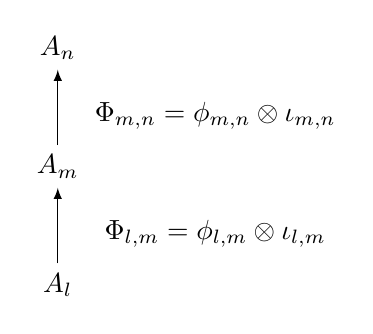
\begin{tikzpicture}
      \node (l) at (0, 0) {$A_l$};
      \node (m) at (0, 1.5) {$A_m$};
      \node (n) at (0, 3) {$A_n$};

      \draw[arrow] (l) -- (m);
      \draw[arrow] (m) -- (n);

      \node (f12) at (2, 0.65)
      {$\Phi_{l,m}=\phi_{l, m}\otimes\iota_{l, m}$};
      \node (f13) at (2, 2.15)
      {$\Phi_{m,n}=\phi_{m, n}\otimes\iota_{m, n}$};
    \end{tikzpicture}
\end{center}
Now the map $\Phi_{m, m}\circ\Phi_{l,m}$ is a Kummer embedding from $A_l$ into
$A_n$, hence there exist an embedding
$\phi:\mathbb{F}_{p^{l}}\emb\mathbb{F}_{p^{n}}$ such that 
\[
  \Phi_{m, m}\circ\Phi_{l,m}=\phi\otimes\iota_{l, n}.
\]
But we also have 
\[
  \Phi_{m, m}\circ\Phi_{l,m}=(\phi_{m, n}\circ\phi_{l,
  m})\otimes(\iota_{m, n}\circ\iota_{l, m}),
\]
and since $\iota_{l,n}=\iota_{m, n}\circ\iota_{l, m}$ by definition, we obtain
\[
  \phi_{m, n}\circ\phi_{l, m}=\phi,
\]
thus the correspondence commutes with compositions of embeddings.
\end{proof}
\begin{prop}
  \label{prop:correspondence-solutions}
  Let $\alpha_m\in A_m$ be a nonzero solution of~\eqref{eq:h90-kummer} for
  $\zeta_m$, and let $c_m$ be its Kummer constant. Then, there is a $1$-to-$1$
  correspondence between Kummer embeddings
  \[
    \Phi:A_l\emb A_m
  \]
  and solutions $\hat\alpha\in A_n$ of~\eqref{eq:h90-kummer} for
  $(\zeta_n)^{n/m}=\iota_{m, n}(\zeta_m)$ that also satisfy
  \[
    \hat\alpha^m = 1\otimes\iota_{m, n}(c_m).
  \]
  The correspondence is given by
  \[
    \Phi(\alpha_m)\longleftrightarrow \hat\alpha.
  \]
\end{prop}
\begin{proof}
Let $\Phi:A_m\emb A_n$ be a Kummer embedding. Lemma~\ref{lm:h90-solutions} shows
that $\alpha_m$ is a generator of $A_m$ as an $1\otimes\mathbb{F}_{p}(\zeta_m)$
algebra. Thus every element $\beta\in A_m$ can be written in the form
\[
  \beta = \sum_{j=0}^{m-1}(1\otimes b_j)(\alpha_m)^j,
\]
and we obtain
\[
  \Phi(\beta) = \sum_{j=0}^{m-1}(1\otimes\iota_{m, n}(b_j))\Phi(\alpha_m)^j,
\]
therefore we see that $\Phi$ is determined by its image $\Phi(\alpha_m)$. Moreover,
$\hat\alpha=\Phi(\alpha_m)$ is a solution of~\eqref{eq:h90-kummer} for
$(\zeta_n)^{n/m}=\iota_{m,n}(\zeta_m)$ that satisfies
$\hat\alpha^m=\iota_{m, n}(c_m)$. Indeed, this is a generalization of the
computations done in Section~\ref{sec:kummer-algebras} and a consequence of
Definition~\ref{defi:kummer-embedding}. We have
\begin{align*}
 (\sigma\otimes1)(\hat\alpha) &=(\sigma\otimes1)(\Phi(\alpha_m))\\
 &= \Phi( (\sigma\otimes1)(\alpha_m))\\
 &= \Phi((1\otimes\zeta_m)\alpha_m)\\
 &= (1\otimes\iota_{m, n})(\zeta_m)\Phi(\alpha_m)\\
 &= (1\otimes\iota_{m, n}(\zeta_m))\hat\alpha
\end{align*}
and
\begin{align*}
 \hat\alpha^m &= \Phi(\alpha_m)^m\\
 &= \Phi(\alpha_m^m)\\
 &= \Phi(1\otimes c_m)\\
 &= 1\otimes\iota_{m, n}(c_m).
\end{align*}

 Converserly, if $\hat\alpha$ is a solution of~\eqref{eq:h90-kummer} for
 $\iota_{m, n}(\zeta_m)$ such that $\hat\alpha^m=\iota_{m, n}(c_m)$, we see that
 \[
  \Phi(\beta) = \sum_{j=0}^{m-1}(1\otimes\iota_{m, n}(b_j))\hat\alpha^j,
 \]
 for any element
 \[
  \beta = \sum_{j=0}^{m-1}(1\otimes b_j)(\alpha_m)^j
 \]
 gives a well-defined morphism of algebras from  $A_m$ into $A_n$ that satisfies
 $\Phi(\alpha)=\hat\alpha$ and
 the conditions in Definition~\ref{defi:kummer-embedding}, \ie it extends
 $\iota_{m, n}$ and commutes with $\sigma\otimes1$.
\end{proof}
With these two correspondences, we can now describe a little more the link
between solutions of~\eqref{eq:h90-kummer} and the finite field embeddings
$\phi$ that we compute from them.
\begin{cor}
  \label{cor:link-h90-embedding}
  Let $\alpha_m\in A_m$ be a nonzero solution of~\eqref{eq:h90-kummer} for
  $\zeta_m$ with Kummer constant $c_m$ and let $\hat\alpha\in A_n$ be a solution
  of~\eqref{eq:h90-kummer} for $(\zeta_n)^{n/m}$ that satisfies
  $\hat{\alpha}^m=\iota_{m, n}(c_m)$. Then
  \begin{itemize}
    \item the solution $\hat{\alpha}$ belongs to the subset
      $\mathbb{F}_{p^{l}}\otimes\mathbb{F}_p((\zeta_n)^{n/m})\subset A_n$;
    \item the assignation
      $\first{\alpha_m}{\zeta_m}\mapsto\first{\hat\alpha}{(\zeta_n)^{n/m}}$
      defines an embedding $\phi:\mathbb{F}_{p^{m}}\emb\mathbb{F}_{p^{n}}$;
    \item the map $\Phi=\phi\otimes\iota_{m, n}$ is the unique Kummer embedding
      such that $\Phi(\alpha_m)=\hat\alpha$.
  \end{itemize}
\end{cor}
\begin{proof}
  By Proposition~\ref{prop:correspondence-solutions}, we know that there exists
  a unique Kummer embedding 
  \[
    \Phi:A_m\emb A_n
  \]
  such that $\Phi(\alpha_m) =
  \hat\alpha$. We also know thanks to
  Proposition~\ref{prop:correspondence-embeddings} that
  \[
    \Phi=\phi\otimes\iota_{m, n}
  \]
  for some embedding of finite fields
  $\phi:\mathbb{F}_{p^{m}}\emb\mathbb{F}_{p^{n}}$. If $\alpha_m =
  \sum_{j=0}^{a-1}x_j\otimes(\zeta_m)^j$, where $a$ is the level of $A_m$, we
  obtain
  \[
    \hat\alpha = \sum_{j=0}^{a-1}\phi(x_j)\otimes(\zeta_n)^{\frac{in}{m}},
  \]
  thus we have $\hat\alpha\in\mathbb{F}_{p^{m}}\otimes\mathbb{F}_{p}(
  (\zeta_n)^{n/m})$. We also see that $x_0=\first{\alpha_m}{\zeta_m}$ is mapped
  to $\phi(x_0) = \first{\hat\alpha}{(\zeta_n)^{n/m}}$, but
  $\first{\alpha_m}{\zeta_m}$ is a generating element of
  $\mathbb{F}_{p^{m}}$ by Proposition~\ref{prop:generate}, hence the assignation
  \[
    \first{\alpha_m}{\zeta_m}\mapsto\first{\hat\alpha}{(\zeta_n)^{n/m}}
  \]
  defines $\phi$.
\end{proof}
With these results we are ready to generalize
Proposition~\ref{prop:lenstra-allombert-algorithm} to the embedding case, with
the cyclotomic lattice setting, giving a minor variation of the original
algorithm of Allombert.
\begin{algorithm}
  \caption{(Allombert's algorithm)}
  \label{algo:allombert}
  \begin{algorithmic}[1]
    \Require{$\mathbb{F}_{p^m}, \mathbb{F}_{p^n}$, for $m\mid n$ integers prime to $p$,
    and a cyclotomic lattice $\mathcal S^{\{l,m\}}$.}
    \Ensure{$s\in \mathbb{F}_{p^m}, t\in\mathbb{F}_{p^n}$, such that the assignation $s\mapsto t$
    defines an embedding $\phi:\mathbb{F}_{p^{m}}\emb\mathbb{F}_{p^n}$.}
  \State Construct the Kummer algebras $A_m$ and $A_n$.
  \State Find $\alpha_m\in A_m$ and $\alpha_n\in A_n$, nonzero solutions
  of~\eqref{eq:h90-kummer} for $\zeta_m$
  and $\zeta_n$ respectively.
  \State Compute their Kummer constants: $(\alpha_m)^m=1\otimes c_m$ and
  $(\alpha_n)^n=1\otimes c_n$.
  \State Compute $\kappa$, a $m$-th root of $\iota_{m, n}(c_m)/c_n$.
  \State Return $\first{\alpha_{m}}{\zeta_m}$ and
  $\first{(1\otimes\kappa)(\alpha_n)^{\frac{n}{m}}}{(\zeta_n)^{\frac{n}{m}}}$.
  \end{algorithmic}
\end{algorithm}
\begin{prop}
  \label{prop:allombert-works}
  Algorithm~\ref{algo:allombert} is correct: it returns elements that define an
  embedding $\phi:\mathbb{F}_{p^{m}}\emb\mathbb{F}_{p^{n}}$.
\end{prop}
\begin{proof}
  The ideas of the proof are the same as the ones found in the proof of
  Proposition~\ref{prop:lenstra-allombert-algorithm}, which were already present
  in the simpler case of Proposition~\ref{prop:allombert-simple}, where all the
  roots of unity are in $\K$. By
  Proposition~\ref{prop:correspondence-embeddings}, let 
  \[
    \Phi=\phi\otimes\iota_{m, n}
  \]
  be a Kummer embedding from $A_m$ into $A_n$. Let $\alpha_m\in A_m$ a solution
  of~\eqref{eq:h90-kummer} for $\zeta_m$ with Kummer constant $c_m$, and let
  $\alpha_n\in A_n$ a solution of~\eqref{eq:h90-kummer} for $\zeta_n$ with
  Kummer constant $c_n$. By
  Proposition~\ref{prop:correspondence-solutions}, there is a solution $\hat\alpha\in
  A_n$ of~\eqref{eq:h90-kummer} for $(\zeta_n)^{n/m}$ that satisfies
  $\hat{\alpha}^m=\iota_{m, n}(c_m)$ and such that $\Phi(\alpha_m)=\hat\alpha$.
  Now, we also have that $(\alpha_n)^{n/m}$ is a solution
  of~\eqref{eq:h90-kummer} for $(\zeta_n)^{n/m}$, and the solutions
  of~\eqref{eq:h90-kummer} for $(\zeta_n)^{n/m}$ form a one-dimensional
  $1\otimes\mathbb{F}_{p}(\zeta_n)$-vector space, so there exists a constant
  $\lambda\in\mathbb{F}_{p}(\zeta_n)$ such that
  \[
    \hat\alpha = (1\otimes\lambda)(\alpha_n)^{n/m}.
  \]
  We conclude that 
  \[
    \cfrac{\iota_{m, n}(c_m)}{c_n} = \lambda^m
  \]
  is a $m$-th root in $\mathbb{F}_{p}(\zeta_n)$. If we let
  \[
    \kappa = (\zeta_n)^{\frac{in}{m}}\lambda,
  \]
  for some integer $i$, be a $m$-th root of $\frac{\iota_{m, n}(c_m)}{c_n}$, it
  follows that
  \[
    \tilde\alpha = (1\otimes\kappa)(\alpha_n)^{n/m} =
    (1\otimes(\zeta_n)^{\frac{in}{m}})\hat\alpha
  \]
  is a solution of~\eqref{eq:h90-kummer} for $(\zeta_n)^{n/m}$ that satisfies
  $\tilde\alpha^m = \iota_{m,n}(c_m)$. By
  Corollary~\ref{cor:link-h90-embedding}, we know that the assignation
  \[
    \first{\alpha_m}{\zeta_m}\mapsto\first{\tilde\alpha}{(\zeta_n)^{n/m}}
  \]
  defines an embedding from $\mathbb{F}_{p^m}$ into $\mathbb{F}_{p^{n}}$.
\end{proof}
\begin{rem}
  Taking the same notations as the one in the proof of
  Proposition~\ref{prop:allombert-works}, we see that the embedding returned by
  the algorithm is $\sigma^i\circ\phi$. Indeed, we have
  \begin{align*}
    \tilde\alpha &= (1\otimes(\zeta_n)^{\frac{in}{m}})\hat\alpha\\
    &= (\sigma\otimes1)^i(\hat\alpha)\\
    &= (\sigma^i\otimes1)(\hat\alpha).
  \end{align*}
  If we let $x_0=\first{\hat\alpha}{(\zeta_n)^{\frac{n}{m}}}$, we wee that the
  returned embedding is defined by the assignation
  \[
    \first{\alpha_m}{\zeta_m}\mapsto\sigma^i(x_0)
  \]
  while $\phi$ is defined by
  \[
    \first{\alpha_m}{\zeta_m}\mapsto x_0.
  \]
\end{rem}
\section{Standard solution of Hilbert $90$}
\label{sec:standard-solution}

\subsection{Complete algebras and standardization}
\label{sec:standardization}

We discussed in Section~\ref{sec:iso-to-emb} the 
obstacles when constructing a lattice of compatibly embedded finite fields using
Lenstra-Allombert algorithm. The first one is that we need to have compatibility
between the roots of unity that we use, and that can be hard to obtain in
practice. We solved that problem by assuming the availability of a
cyclotomic lattice $\mathcal S^I$, and we proved that all the results concerning
Lenstra-Allombert can be expressed in that setting in
Section~\ref{sec:kummer-embeddings}. Now, we can obtain compatibility by
replacing the naive embedding algorithm by Lenstra-Allombert algorithm in
Bosma-Canon-Steel framework. This solutions immediately gives a compatible
lattice of embedded finite fields. Still, among the sub-goals presented in
Section~\ref{sec:compatibility-problem} that such a lattice may achieve, there
are two of them on which we would like to improve.
\begin{description}
  \item[\emph{Uniqueness:}] the element $\first{\lambda_m}{\zeta_m}$ is
    a generator of $\mathbb{F}_{p^{m}}$, or equivalently, it provides an
    irreducible polynomial in $\K[X]$ of degree $m$. However this polynomials
    depends on the choice of $\alpha_l$, because it depends on the Kummer constant
    $c_l$ of $\alpha_l$ by Proposition~\ref{prop:kummer-constant}, thus there is
    no uniqueness.
  \item[\emph{Compatibility:}] the embedding of finite fields
    $\phi:\mathbb{F}_{p^{m}}\to\mathbb{F}_{p^{n}}$ depends on
    the choice of the constant $\kappa$, which itself depends on the choice of
    the solutions $\alpha_m$ and $\alpha_n$ of \eqref{eq:h90-kummer}, and also
    of the choice of a $m$-th root of unity. In order to achieve compatibility,
    we must keep track of the constants $\kappa$ for each embedding computation
    \[
      \mathbb{F}_{p^{m}}\emb\mathbb{F}_{p^{n}}
    \]
    in the
    lattice, which grow quadratically with the number of fields, because of the
    common subfield compatibility condition in Bosma-Canon-Steel framework.
\end{description}
In this section and in Section~\ref{sec:standard-embeddings}, we will see how to
choose special solutions of \eqref{eq:h90-kummer}, in order to manage these
constants $\kappa$. Our dream would be to be able to choose the solutions
of~\eqref{eq:h90-kummer} in a way that makes the constants trivial, \ie 
\[
  \kappa_{\mathbb{F}_{p^{m}}\emb \mathbb{F}_{p^{n}}} = 1.
\]
From Algorithm~\ref{algo:allombert}, we see that the constant
$\kappa_{\mathbb{F}_{p^{m}}\emb\mathbb{F}_{p^{n}}}$ is a $m$-th root of the
quotient
\[
  \cfrac{\iota_{m, n}(c_m)}{c_n},
\]
thus the condition $\kappa_{\mathbb{F}_{p^{m}}\emb\mathbb{F}_{p^{n}}}=1$ implies
\[
  \iota_{m, n}(c_m) = c_n,
\]
which in turn implies that $c_n$ belongs to the subset
\[
  \mathbb{F}_{p}( (\zeta_n)^{\frac{n}{m}})\subseteq\mathbb{F}_p(\zeta_n).
\]
This could possibly fail if the Kummer algebras $A_m$ and $A_n$ are of distinct
level, \ie if their field of scalars are different. This motivates the study of
Kummer algebras of a given level, and the introduction of the notion of
\emph{complete} algebra.
\begin{defi}[Complete Kummer algebra]
  A Kummer algebra is \emph{complete} if it is of the largest degree for a given
  level.
\end{defi}
Therefore, the complete Kummer algebra of level $a$ is the Kummer algebra
\begin{align*}
  A_{p^a-1} &=
  \mathbb{F}_{p^{p^a-1}}\otimes\mathbb{F}_p(\zeta_{p^a-1})\\
  &=\mathbb{F}_{p^{p^a-1}}\otimes\mathbb{F}_{p^{a}}
\end{align*}
with field of scalar
\[
  \mathbb{F}_{p^{a}}\cong \mathbb{F}_p(\zeta_{p^a-1}).
\]
given by the element $\zeta_{p^a-1}$ in the cyclotomic lattice $\mathcal S^I$.
In fact these algebras have an interesting property.
\begin{lm}
  All nonzero solutions $\alpha_{p^a-1}\in A_{p^a-1}$ of~\eqref{eq:h90-kummer}
  for $\zeta_{p^a-1}$ have the same Kummer constant
  \[
    c_{p^a-1} = (\zeta_{p^a-1})^{a}.
  \]
\end{lm}
\begin{proof}
  \label{lm:complete-algebra-solutions}
  Let $\alpha_{p^a-1}\in A_{p^a-1}$ a solution of~\eqref{eq:h90-kummer} for
  $\zeta_{p^a-1}$. For all $\beta\in A_{p^a-1}$, we have $\beta^p = \sigma\otimes\sigma(\beta) =
  \beta^p$, so we also obtain 
  \[
    (\alpha_{p^a-1})^{p^a} = (\sigma^a\otimes\sigma^a)(\alpha_{p^a-1}).
  \]
  Now, we know that $\sigma^a$ is the identity on $\mathbb{F}_{p^a}$, hence we
  have
  \begin{align*}
    (\alpha_{p^a-1})^{p^a} &= (\sigma^a\otimes1)(\alpha_{p^a-1}) \\
    &= (1\otimes\zeta_{p^a-1})^a \alpha_{p^a-1}.
  \end{align*}
  Since $\alpha_{p^a-1}$ is invertible by Lemma~\ref{lm:h90-solutions}, we
  obtain that
  \[
    (\alpha_{p^a-1})^{p^a-1} = 1\otimes c_{p^a-1} = (1\otimes \zeta_{p^a-1})^a
  \]
  and it follows that
  \[
    c_{p^a-1} = (\zeta_{p^a-1})^{a}.
  \]
\end{proof}
Now this result is very important because we know that the degree $p^a-1$
irreducible polynomial in $\K[X]$ derived from the solution $\alpha_{p^a-1}$,
\ie the minimal polynomial of the element
$\first{\alpha_{p^a-1}}{\zeta_{p^a-1}}$,
only depends on the Kummer constant $c_{p^a-1}$ of $\alpha_{p^a-1}$, thus it
means that all solutions give the same polynomial. This will be the central idea
behind the notion of \emph{standard} elements.
\begin{defi}[Standard Kummer constant]
  Let $m$ be an integer prime to $p$. We define the \emph{standard Kummer
  constant} of order $m$ as
  \[
    \stdc{m} = (\iota_{m,
    p^a-1})^{-1}((\zeta_{p^a-1})^a)\in\mathbb{F}_{p}(\zeta_m),
  \]
  where $a=\nu(m)$ is the level of the Kummer algebra $A_m$.
\end{defi}
\begin{rem}
 Since $A_m$ is of level $a$, we have
 \[
   \mathbb{F}_p(\zeta_m) \cong \mathbb{F}_p(\zeta_{p^a-1}),
 \]
 hence the map $\iota_{m, p^a-1}$ is an isomorphism and $\stdc{m}$ is
 well-defined.
\end{rem}
\begin{defi}[Standard solution]
  Let $m$ be an integer prime to $p$. We say that a solution $\alpha_m\in A_m$
  is \emph{standard} if its Kummer constant is standard, \ie if we have
  \[
    (\alpha_m)^m = 1\otimes\stdc{m}.
  \]
\end{defi}
\begin{defi}[Decorated Kummer algebra]
  Let $m$ be an integer prime to $p$. We define a \emph{decorated Kummer
  algebra} as a couple
  \[
    (A_m, \alpha_m),
  \]
  where $\alpha_m$ is a standard solution of~\eqref{eq:h90-kummer} for
  $\zeta_m$.
\end{defi}
It follows from Lemma~\ref{lm:complete-algebra-solutions} that all nonzero
solutions of~\eqref{eq:h90-kummer} in a complete algebra are standard. This is
no longer the case in a non complete Kummer algebra, but we can still find
standard solutions.
\begin{prop}
  \label{prop:decoration}
 Let $m$ an integer prime to $p$. Then $A_m$ can be decorated, \ie it admits a
 standard solution $\alpha_m$. Moreover, this solution $\alpha_m$ is unique up
 to a $m$-th root of unity. 
\end{prop}
\begin{proof}
 Let $a=\nu(m)$ be the level of $A_m$ and let $\alpha_m'\in A_m$ be a nonzero solution
 of~\eqref{eq:h90-kummer} for $\zeta_m$. Let also $\alpha_{p^a-1}$ be a nonzero
 solution of~\eqref{eq:h90-kummer} for $\zeta_{p^a-1}$, then it is standard by
 Lemma~\ref{lm:complete-algebra-solutions}. The element 
 \[
   (\alpha_{p^a-1})^{\frac{p^a-1}{m}}
 \]
 is a solution of~\eqref{eq:h90-kummer} for
 \[
   \iota_{m, p^a-1}(\zeta_m) = (\zeta_{p^a-1})^{\frac{p^a-1}{m}}.
 \]
 Now let
 \[
   \Phi:A_m\emb A_{p^a-1}
 \]
 be a Kummer embedding and let
 \[
   \hat\alpha = \Phi(\alpha_m'),
 \]
 then $\hat\alpha$ is also a solution of~\eqref{eq:h90-kummer} for
 $\iota_{m, p^a-1}(\zeta_m)$ and thus there exists a scalar
 $\lambda\in\mathbb{F}_p(\zeta_{p^a-1})$ such that
 \[
   (\alpha_{p^a-1})^{\frac{p^a-1}{m}} = (1\otimes\lambda)\hat{\alpha} .
 \]
 If we let
 \[
   \tilde\lambda = \iota_{m, p^a-1}^{-1}(\lambda),
 \]
 we obtain
 \begin{align*}
   (\alpha_{p^a-1})^{\frac{p^a-1}{m}} &= (1\otimes\lambda)\Phi(\alpha_m') \\
   &= \Phi( (1\otimes\tilde\lambda)\alpha_m').
 \end{align*}
If we set 
\[
  \alpha_m = (1\otimes\tilde\lambda)\alpha_m',
\]
it follows that
\begin{align*}
  \Phi((\alpha_m)^m) &= (\alpha_{p^a-1})^{p^a-1} \\
  &= 1\otimes(\zeta_{p^a-1})^a,
\end{align*}
therefore
\begin{align*}
  (\alpha_m)^m &= 1\otimes\iota_{m, p^a-1}^{-1}( (\zeta_{p^a-1})^a) \\
  &= 1 \otimes \stdc{m}
\end{align*}
and $\alpha_m$ is standard. If $\beta\in A_m$ is another solution
of~\eqref{eq:h90-kummer} for $\zeta_m$, then there exists a scalar
$\mu\in\mathbb{F}_p(\zeta_m)$ such that
\[
  \alpha_m= (1\otimes\mu)\beta,
\]
but then we obtain
\[
  (\alpha_m)^m = (1\otimes\mu^m)\beta^m.
\]
As a consequence, $\beta$ is standard if and only if $\mu^m = 1$ and the
standards solutions are the
\[
  (1\otimes\zeta_m^u)\alpha_m
\]
for $0\leq u\leq m-1$.
\end{proof}
From Proposition~\ref{prop:decoration}, it follows that for any integer $m$
prime to $p$, we can define $\mathbb{F}_{p^{m}}$ in a standard way.
\begin{defi}[Standard generating element]
  A generating element $x\in\mathbb{F}_{p^{m}}$ is called \emph{standard} if it
  is of the form
  \[
    x = \first{\alpha_m}{\zeta_m}
  \]
  for $\alpha_m\in A_m$ a standard solution of~\eqref{eq:h90-kummer}.
\end{defi}
\begin{defi}[Standard defining polynomial]
  The \emph{standard defining polynomial} $P_m$ for $\mathbb{F}_{p^{m}}$ is the
  minimal polynomial over $\K$ of a standard generating element of
  $\mathbb{F}_{p^{m}}$.
\end{defi}
\begin{defi}[Decorated finite field]
  Let $m\in\mathbb{N}$ an integer prime to $p$. A \emph{decorated finite field}
  is a couple $(\mathbb{F}_{p^{m}}, s_m)$ where $s_m\in\mathbb{F}_{p^{m}}$ is a
  standard generating element.
\end{defi}
\begin{rem}
  By Remark~\ref{rem:recover-alpha}, we can recover $\alpha_m$ the standard
  solution of~\eqref{eq:h90-kummer} from the standard generating element $s_m$,
  thus decorated Kummer algebras can be recovered from
  decorated finite fields.
\end{rem}
By Proposition~\ref{prop:kummer-constant}, we know that $P_m$ is entirely 
determined by $\stdc{m}$, and thus by the cyclotomic lattice $\mathcal S^I$ up
to order $p^a-1$, with $a=\nu(m)$ the level of $m$. This helps to achieve the
\emph{uniqueness} sub-goal of our lattice, because once the cyclotomic lattice
has been chosen, the standard defining polynomials are unique. As an example, we
give in Table~\ref{tab:std-polys} the first ten standard defining polynomials
induced by the cyclotomic lattice given by the Conway polynomials with $p=2$.
\begin{table}
  \centering
  \begin{tabular}{l}
    $x+1$ \\
    $x^3+x+1$ \\
    $x^5+x^3+1$ \\
    $x^7+x+1$ \\
    $x^9+x^7+x^4+x^2+1$\\
    $x^{11}+x^8+x^7+x^6+x^2+x+1$\\
    $x^{13}+x^{10}+x^5+x^3+1$\\
    $x^{15}+x+1$ \\
    $x^{17}+x^{11}+x^{10}+x^8+ x^7+x^6+x^4+x^3+x^2+x+1$ \\
    $x^{19}+x^{17}+x^{16}+x^{15}+x^{14}+x^{13}+x^{12}+x^8+x^7+x^6+x^5+x^3+1$
  \end{tabular}
  \caption{The first ten standard polynomials derived from Conway
    polynomials for $p=2$.}
  \label{tab:std-polys}
\end{table}
A small variation of Lenstra-Allombert algorithm, given by
Algorithm~\ref{algo:decoration}, allows us to compute all these standard
elements.
\begin{algorithm}
  \caption{(Decoration -- Standardization)}
  \label{algo:decoration}
  \begin{algorithmic}[1]
    \Require {$\mathbb{F}_{p^m}$, for $m$ prime to $p$, and $\mathcal{S}^I$ a cyclotomic lattice.}
    \Ensure {$(A_m,\alpha_m)$ decorated, $P_m$ standard irreducible polynomial of degree $m$,
      and $s\in\mathbb{F}_{p^m}$ standard generating element inducing $\mathbb{F}_{p^m}\simeq\mathbb{F}_{p}[T]/(P_m)$.}
  \State Compute the Kummer algebra $A_m$.
  \State Compute $\stdc{m}=(\iota_{m, p^a-1})^{-1}((\zeta_{p^a-1})^a)\in\mathbb{F}_p(\zeta_m)$.
  \State Find $\alpha'_m\in A_m$ a nonzero solution of~\eqref{eq:h90-kummer} for $\zeta_m$.
  \State Compute its Kummer constant: $(\alpha'_m)^m=1\otimes c'_m$.
  \State Compute $\kappa$ a $m$-th root of $\stdc{m}/ c'_m$.
  \State Set $\alpha_{m}=(1\otimes\kappa)\alpha'_m$.
  \State Compute $P_m$ the minimal polynomial of $\first{\alpha_{m}}{\zeta_m}$
  over $\K$.
  \State Return $(A_m,\alpha_m)$, $P_m$, and $\first{\alpha_m}{\zeta_m}$.
  \end{algorithmic}
\end{algorithm}
\begin{prop}
  Algorithm~\ref{algo:decoration} is correct, \ie the computed element
  $\alpha_m$ is indeed standard. 
\end{prop}
\begin{proof}
  By Proposition~\ref{prop:decoration}, we know that there exists a standard
  solution of~\eqref{eq:h90-kummer} for $\zeta_m$, let $\pmb{\alpha}\in A_m$ be such a
  solution. Let $\alpha_m'\in A_m$ be any nonzero solution
  of~\eqref{eq:h90-kummer} for $\zeta_m$ and let $c_m'$ be its Kummer constant.
  Then we know that there exists $\lambda\in\mathbb{F}_p(\zeta_m)$ a scalar such that
  \[
    \pmb\alpha = (1\otimes\lambda)\alpha_m'.
  \]
  It follows that 
  \[
    \stdc{m} = \lambda^m c_m',
  \]
  thus 
  \[
    \stdc{m}/c_m'
  \]
  is indeed a $m$-th power. If we let $\kappa$ be a $m$-th root of
  $\stdc{m}/c_m'$ and if we set 
  \[
    \alpha_m = (1\otimes\kappa)\alpha_m',
  \]
  we obtain
  \[
    (\alpha_m)^m = 1\otimes\stdc{m}.
  \]
  We have thus proven that $\alpha_m$ is a standard solution
  of~\eqref{eq:h90-kummer} for $\zeta_m$. By definition,
  $\first{\alpha_m}{\zeta_m}$ is then a standard generating element of
  $\mathbb{F}_{p^{m}}$ and its minimal polynomial $P_m$ is a standard defining
  polynomial.
\end{proof}

\subsection{Towards standard embeddings}
\label{sec:towards-standard-embeddings}

Now that we have found a way to compute standard solutions
of~\eqref{eq:h90-kummer}, and to deduce standard generating elements to define
our finite fields, it is natural to work towards the definition of compatible
embeddings between these finite fields that are also standard. Our goal is also
to simplify the storage of the constants $\kappa$ involved in the computation of
such embeddings.
\begin{prop}
  \label{prop:power-compatibility}
  Let $m\mid n$ be two integers prime to $p$ and such that 
  \[
    \nu(m) = \nu(n),
  \]
  \ie the (decorated) Kummer algebras $(A_m, \alpha_m)$ and $(A_n, \alpha_n)$
  have the same level. Then there is a unique Kummer embedding
  \[
    \stdemb{m}{n}:A_m\emb A_n
  \]
  such that
  \[
    \stdemb{m}{n}(\alpha_m) = (\alpha_n)^{\frac{n}{m}}.
  \]
\end{prop}
\begin{proof}
  The element $\hat\alpha = (\alpha_n)^{\frac{n}{m}}$ is a solution
  of~\eqref{eq:h90-kummer} for $(\zeta_n)^{\frac{n}{m}}=\iota_{m, n}(\zeta_m)$.
  We also know that the Kummer constant of $\alpha_m$ is
  \[
    \stdc{m} = \iota_{m, p^a-1}^{-1}((\zeta_{p^a-1})^a)
  \]
  and the Kummer constant of $\alpha_n$ is 
  \[
    \stdc{n} = \iota_{n, p^a-1}^{-1}((\zeta_{p^a-1})^a).
  \]
  The embeddings $\iota$ are compatible by definition, thus we have
  \[
    \iota_{m, p^a-1} = \iota_{n, p^a-1}\circ\iota_{m, n}
  \]
  and
  \[
    \iota_{n, p^a-1}^{-1} = \iota_{m, n}\circ\iota_{m, p^a-1}^{-1}.
  \]
  It follows that
  \[
    \stdc{n} = \iota_{m, n}(\stdc{m}).
  \]
  By Proposition~\ref{prop:correspondence-solutions}, there exists a unique
  Kummer embedding $\stdemb{m}{n}$ such that
  \[
    \stdemb{m}{n}(\alpha_m) = \hat\alpha = (\alpha_n)^{\frac{n}{m}}.
  \]
\end{proof}
Proposition~\ref{prop:power-compatibility} guarantees that decorated Kummer
algebras $(A_m, \alpha_m), (A_n, \alpha_n)$ of the same level are
\emph{power-compatible}, \ie we can describe a unique Kummer embedding by
\[
  \alpha_m\mapsto (\alpha_n)^{\frac{n}{m}}.
\]
Therefore, there is no constant $\kappa$ to store in this case because we are in
the trivial case $\kappa=1$, which was our
goal. However, we see that power compatibility implies
\[
  \stdc{n} = \iota_{m, n}(\stdc{m}),
\]
hence implies that the decorated Kummer algebras share the same level. If the
Kummer algebras do not share the same level, we can ask for
\emph{norm-compatibility} instead of power-compatibility, at least between two
\emph{complete} decorated Kummer algebras. 
Let us first describe what ``norm'' we will be using.
Let $A_n$ be a Kummer algebra of level $\nu(n) = b$, so that
\[
  A_n = \mathbb{F}_{p^{n}}\otimes\mathbb{F}_{p^{b}}\cong
  \mathbb{F}_{p^{n}}\otimes\mathbb{F}_{p}(\zeta_{p^b-1}),
\]
where the isomorphism is given by $1\otimes\iota_{n, p^b-1}$. Then, if $a\mid b$
is another integer, the subalgebra of $A_n$ invariant under $1\otimes\sigma^a$
is identified (by the same isomorphism) with
\[
  (A_n)^{1\otimes\sigma^a} \cong \mathbb{F}_{p^{n}}\otimes\mathbb{F}_p(
  (\zeta_{p^b-1})^{\frac{p^b-1}{p^a-1}})
\]
where
\[
  (\zeta_{p^b-1})^{\frac{p^b-1}{p^a-1}} =
  N_{\mathbb{F}_{p^{n}}/\mathbb{F}_{p^{a}}}(\zeta_{p^b-1}) = \iota_{p^a-1,
  p^b-1}(\zeta_{p^a-1})
\]
and where $N_{\mathbb{F}_{p^{n}}/\mathbb{F}_{p^{a}}}$ is the relative norm of
the finite field extension
\[
  \mathbb{F}_{p^{b}}/\mathbb{F}_{p^{a}}.
\]
\begin{defi}[Scalar norm operator]
  Let $n$ an integer prime to $p$ and $A_n$ a Kummer algebra of level
  $\nu(n)=c$. Let $a,b$ two integers such that $a\mid b \mid c$,
  then we define the \emph{scalar norm operator} as
  \[
    \begin{array}{cccc}
      \mathcal N_{b/a,\, A_n}: & (A_n)^{1\otimes\sigma^b} & \to &
      (A_n)^{1\otimes\sigma^a}\\
      & \gamma & \mapsto & \prod_{0\leq j\leq
        \frac{a}{b}}(1\otimes\alpha^{ja})(\gamma)
    \end{array}
  \]
\end{defi}
This operator is well-defined, as the elements in the image of $\mathcal
N_{b/a,\, A_n}$ are indeed invariant under $1\otimes\sigma^a$. We often 
omit $A_n$ and only write $\N_{b/a}$, as the ambient space $A_n$ is
implicit. By construction, $\N_{b/a}$ acts on the scalar field
$1\otimes\mathbb{F}_{p^b}^\times$ as the usual norm $1\otimes
N_{\mathbb{F}_{p^{b}}/\mathbb{F}_{p^{a}}}$. Scalar norms are
\emph{multiplicative}, \ie for any $\gamma, \gamma'\in A_n$, we have
\[
  \N_{b/a}(\gamma\gamma') = \N_{b/a}(\gamma)\N_{b/a}(\gamma'),
\]
they are \emph{transitive}, \ie for any $a\mid b\mid c$, we have
\[
  \N_{c/a} = \N_{b/a}\circ\N_{c/b},
\]
and they commute with $\sigma\otimes1$. All these nice properties make the
scalar norm an excellent candidate to generalize the powering used to define
standard embeddings between decorated Kummer algebras of same level.
\begin{prop}
  \label{prop:norm-compatibility}
  Let $a\mid b$ be two integers prime to $p$ and let $(A_{p^a-1},
  \alpha_{p^a-1})$, $(A_{p^b-1}, \alpha_{p^b-1})$ two decorated complete
  Kummer algebras of levels $a$ and $b$ respectively. Then there is a unique
  Kummer embedding (that we again call \emph{standard})
  \[
    \stdemb{p^a-1}{p^b-1}:A_{p^a-1}\emb A_{p^b-1}
  \]
  such that
  \[
    \stdemb{p^a-1}{p^b-1}(\alpha_{p^a-1}) = \N_{b/a}(\alpha_{p^b-1}).
  \]
\end{prop}
\begin{proof}
  Let $\hat\alpha = \N_{b/a}(\alpha_{p^b-1})$, by the properties of the scalar
  norm, we have
  \begin{align*}
    (\sigma\otimes1)(\hat\alpha) &=
    (\sigma\otimes1)(\N_{b/a}(\alpha_{p^b-1}))\\
    &= \N_{b/a}( (\sigma\otimes1)(\alpha_{p^b-1}))\\
    &= \N_{b/a}( (1\otimes\zeta_{p^b-1})\alpha_{p^b-1})\\
    &= (1\otimes(\zeta_{p^b-1})^{\frac{p^b-1}{p^a-1}})\N_{b/a}(\alpha_{p^b-1}),
  \end{align*}
  therefore $\hat\alpha$ is a solution of~\eqref{eq:h90-kummer} for
  $(\zeta_{p^b-1})^{\frac{p^b-1}{p^a-1}}$.
  We also have 
  \begin{align*}
    \hat\alpha^{p^a} &= (\sigma^a\otimes\sigma^a)(\hat\alpha)\\
    &= (\sigma^a\otimes\sigma^a)(\N_{b/a}(\alpha_{p^b-1}))\\
    &= (\sigma^a\otimes1)(\N_{b/a}(\alpha_{p^b-1}))\\
    &= \N_{b/a}((\sigma^a\otimes1)(\alpha_{p^b-1}))\\
    &= \N_{b/a}((1\otimes(\zeta_{p^b-1})^a)(\alpha_{p^b-1}))\\
    &= (1\otimes\iota_{p^a-1,\,p^b-1}(\zeta_{p^a-1})^a)\N_{b/a}(\alpha_{p^b-1}),
  \end{align*}
  thus $\hat\alpha$ satisfies
  \[
    \hat\alpha^{p^a-1} = 1\otimes\iota_{p^a-1,\,p^b-1}(\stdc{p^a-1}),
  \]
  and by Proposition~\ref{prop:correspondence-solutions} there is a unique
  embedding such that
  \[
    \stdemb{p^a-1}{p^b-1}(\alpha_{p^b-1}) = \hat\alpha.
  \]
\end{proof}

\section{Standard embeddings}
\label{sec:standard-embeddings}

From Proposition~\ref{prop:power-compatibility}, we learned how to construct a
standard Kummer embedding between two decorated Kummer algebras sharing the same
level, using power compatibility. From Proposition~\ref{prop:norm-compatibility}
we learned how to construct a standard Kummer embedding between two decorated
complete Kummer algebras, using norm compatibility. Our goal is
now to use both results together in order to construct a standard Kummer
embedding between any two decorated Kummer algebras. Consider the general
case where we have two integers
$m\mid n$ not divisible by $p$, set $a=\nu(m)$, $b=\nu(n)$, and consider
the diagram
\begin{equation*}
\label{3cotes}
\begin{CD}
(A_{p^a-1},\alpha_{p^a-1}) @>{\stdemb{p^a-1}{p^b-1}}>> (A_{p^b-1},\alpha_{p^b-1}) \\
@A{\stdemb{m}{p^a-1}}AA @AA{\stdemb{n}{p^b-1}}A\\
(A_m,\alpha_m) @. (A_n,\alpha_n)
\end{CD}
\end{equation*}
of standard embeddings of decorated algebras.
\begin{lm}
  \label{lm:existence-embedding}
  In this setting, there exists a unique Kummer embedding
  \[
    \stdemb{m}{n}:A_m\emb A_n
  \]
  that makes the diagram commute. We call this embedding the \emph{standard
  Kummer embedding} from $A_m$ to $A_n$.
\end{lm}
\begin{proof}
  Let
  \[
    \tilde\alpha = \stdemb{p^a-1}{p^b-1}(\stdemb{m}{p^a-1}(\alpha_l))\in
    A_{p^b-1}.
  \]
  The element $\tilde\alpha$ is fixed by both $\sigma^m\otimes1$ and
  $1\otimes\sigma^a$, because $\alpha_m$ is, and Kummer embeddings commute with both
  $\sigma\otimes1$ and $1\otimes\sigma$. Therefore, $\tilde\alpha$ is also fixed
  by $\sigma^n\otimes1$ and $1\otimes\sigma^b$, and thus is in the image of
  $A_n$ by $\stdemb{n}{p^b-1}$. We then let
  \[
    \hat\alpha = (\stdemb{n}{p^b-1})^{-1}(\tilde\alpha)\in A_n.
  \]
  By construction, the element $\tilde\alpha$ is a solution
  of~\eqref{eq:h90-kummer} for
  \[
    \iota_{m,\,p^b-1}(\zeta_m) = (\zeta_{p^b-1})^{\frac{p^b-1}{m}}
  \]
  that satisfies
  \[
    \tilde\alpha^m = 1\otimes\iota_{m,\,p^b-1}(\stdc{m})
  \]
  It thus follows that $\hat\alpha$ is a solution
  of~\eqref{eq:h90-kummer} for 
  \[
    \iota_{n,\,p^b-1}^{-1}(\iota_{m,\,p^b-1}(\zeta_m)) =
    \iota_{m\,n}(\zeta_m)=(\zeta_n)^{\frac{n}{m}}
  \]
  that also satisfies 
  \[
    \hat\alpha^m = 1\otimes\iota_{m,n}(\stdc{m}).
  \]
  By Proposition~\ref{prop:correspondence-solutions}, we then have a unique
  Kummer embedding such that
  \[
    \stdemb{m}{n}(\alpha_m) = \hat\alpha,
  \]
  and that concludes the proof.
\end{proof}
\begin{defi}[Standard embedding]
  Let $m\mid n$ two integers prime to $p$. By
  Proposition~\ref{prop:correspondence-embeddings}, there exists a unique finite
  field embedding 
  \[
    \stdembff{m}{n}:\mathbb{F}_{p^{m}}\emb\mathbb{F}_{p^{n}}
  \]
  such that the standard Kummer embedding $\stdemb{m}{n}$ satisfies
  \[
    \stdemb{m}{n}=\stdembff{m}{n}\otimes\iota_{m,n}.
  \]
  This finite field embedding $\stdembff{m}{n}$ is called the \emph{standard embedding}
  from $\mathbb{F}_{p^{m}}$ to $\mathbb{F}_{p^{n}}$.
\end{defi}
The existence result of Lemma~\ref{lm:existence-embedding} is 
``constructive'', but requires to compute the complete Kummer algebra
$A_{p^a-1}$, that can be very large, thus it is impractical. However, one should
be able to write 
\[
  \hat\alpha = (1\otimes\kappa)(\alpha_n)^{\frac{n}{m}}
\]
for some constant $\kappa\in\mathbb{F}_p(\zeta_n)$,
since both $\hat\alpha$ and $(\alpha_n)^{\frac{n}{m}}$ are solutions
of~\eqref{eq:h90-kummer} for $(\zeta_n)^\frac{n}{m}$. We proved in
Lemma~\ref{lm:existence-embedding} that there was a unique, \emph{standard},
Kummer embedding corresponding to this solution $\hat\alpha$, thus there should
also be a unique constant $\kappa$ corresponding to this embedding. Our aim is
now to give an explicit expression of $\kappa$, so that we do not have to
compute the complete algebra $A_{p^b-1}$ to obtain the Kummer embedding
\[
  \stdemb{m}{n}.
\]
We start with the simpler case of complete algebras nonetheless, \ie we study
the constant $\kappa$ when $m=p^a-1$ and $n=p^b-1$.
\begin{prop}
  \label{prop:link-norm-power}
In the complete algebra $A_{p^b-1}$ we have
\[
(\alpha_{p^b-1})^{\frac{p^b-1}{p^a-1}}=(1\otimes\zeta_{p^b-1})^{\frac{(b-a)
  p^{b+a}-bp^b+ap^a}{(p^a-1)^2}}\norm_{b/a}(\alpha_{p^b-1}).
\]
\end{prop}
\begin{proof}
  Using the fact that $(\sigma\otimes\sigma)(\beta) = \beta^p$ for any $\beta\in
  A_{p^b-1}$, and then~\eqref{eq:h90-kummer}, we get:
  \begin{align*}
\frac{(\alpha_{p^b-1})^{\frac{p^b-1}{p^a-1}}}{\norm_{b/a}(\alpha_{p^b-1})}
&=\prod_{0\leq j<\frac{b}{a}}\frac{(\sigma^{ja}\otimes\sigma^{ja})(\alpha_{
p^b-1})}{(1\otimes\sigma^{ja})(\alpha_{p^b-1})}\\
&=\prod_{0\leq j<\frac{b}{a}}(1\otimes\sigma^{ja})\left(\frac{(\sigma^{ja}
\otimes 1)(\alpha_{p^b-1})}{\alpha_{p^b-1}}\right)\\
&=\prod_{0\leq j<\frac{b}{a}}(1\otimes\sigma^{ja})(1\otimes\zeta_{p^b-1})
^{ja}\\
&=(1\otimes\zeta_{p^b-1})^{\sum_{0\leq j<\frac{b}{a}}jap^{ja}}.
  \end{align*}
We conclude thanks to the identity
\[
\sum_{0\leq j<n}jT^j=T\frac{d}{dT}\!\left(\frac{T^n-1}{T-1}\right)=
\frac{(n-1)T^{n+1}-nT^n+T}{(T-1)^2}.
\]
\end{proof}
From Proposition~\ref{prop:link-norm-power}, we can deduce the constant $\kappa$
involved in the computation of $\stdemb{p^a-1}{p^b-1}$. The results also extends
to non complete algebras.
\begin{cor}
  \label{cor:link-norm-power}
  Let $(A_m, \alpha_n)$ and $(A_n, \alpha_n)$ be two decorated Kummer algebras
  of respective degrees $m\mid n$ prime to $p$ and respective levels $a$ and
  $b$. Then the standard embedding
  \[
    \stdemb{m}{n}:A_m\emb A_n
  \]
  is defined by the assignation
  \[
    \alpha_m\mapsto (1\otimes\kappa_{m, n})(\alpha_n)^{\frac{n}{m}},
  \]
  where 
  \[
    \kappa_{m, n} = \iota_{n,
    p^b-1}^{-1}(\zeta_{p^b-1})^{-\frac{(b-a)p^{b+a}-bp^b+ap^a}{(p^a-1)m}}.
  \]
\end{cor}
\begin{proof}
  Recall that $\stdemb{m}{n}$ is, by construction, the unique Kummer embedding
  that makes the following diagram commute.
\begin{equation*}
\begin{CD}
(A_{p^a-1},\alpha_{p^a-1}) @>{\stdemb{p^a-1}{p^b-1}}>> (A_{p^b-1},\alpha_{p^b-1}) \\
@A{\stdemb{m}{p^a-1}}AA @AA{\stdemb{n}{p^b-1}}A\\
(A_m,\alpha_m) @. (A_n,\alpha_n)
\end{CD}
\end{equation*}
Therefore, if we set
\[
  \hat\alpha = (1\otimes\kappa_{m, n})(\alpha_n)^{\frac{n}{m}},
\]
it is sufficient, by Lemma~\ref{lm:existence-embedding}, to prove that 
\[
  \stdemb{p^a-1}{p^b-1}(\stdemb{m}{p^b-1})(\alpha_m) =
  \stdemb{n}{p^b-1}(\hat\alpha).
\]
However, using Proposition~\ref{prop:norm-compatibility} and
Proposition~\ref{prop:power-compatibility}, we know that
\[
  \stdemb{p^a-1}{p^b-1}(\stdemb{m}{p^b-1})(\alpha_m) =
  \norm_{b/a}(\alpha_{p^b-1})^{\frac{p^a-1}{m}},
\]
and we also know that
\[
  \stdemb{n}{p^b-1}( (\alpha_m)^{\frac{n}{m}}) =
  (\alpha_{p^b-1})^{\frac{p^b-1}{m}}.
\]
Therefore, using Proposition~\ref{prop:link-norm-power}, we obtain
\begin{align*}
  \stdemb{n}{p^b-1}(\hat\alpha) &=   (\zeta_{p^b-1})^{-\frac{(b-a)p^{b+a}
-bp^b+ap^a}{(p^a-1)m}}(\alpha_{p^b-1})^{\frac{p^b-1}{m}}\\
&=( (\zeta_{p^b-1})^{-\frac{(b-a)p^{b+a}
-bp^b+ap^a}{(p^a-1)^2}}(\alpha_{p^b-1})^{\frac{p^b-1}{p^a-1}})^{\frac{p^a-1}{m}}\\
&= \norm_{b/a}(\alpha_{p^b-1})^{\frac{p^a-1}{m}}\\
&= \stdemb{p^a-1}{p^b-1}(\stdemb{m}{p^b-1})(\alpha_m),
\end{align*}
which completes the proof.
\end{proof}
\begin{prop}
  \label{prop:embeddings-compatibility}
  Standard Kummer embeddings are compatible: let $(A_l, \alpha_l), (A_m,
  \alpha_m)$ and $(A_n, \alpha_n)$ three decorated Kummer algebras with
  respective degrees
  \[
    l\mid m\mid n,
  \]
  then the corresponding standard embeddings satisfy
  \[
    \stdemb{l}{n} = \stdemb{m}{n}\circ\stdemb{l}{m}.
  \]
\end{prop}
\begin{proof}
  Corollary~\ref{cor:link-norm-power} gives us explicit formulas for the
  standard Kummer embeddings, thus we can check by direct computation that the
  embeddings are compatible. Let
  \[
    a = \nu(l)\quad b =\nu(m)\quad c = \nu(n)
  \]
  the respective levels of $A_l, A_m$ and $A_n$. Then we have the corresponding
  commutative diagram where the arrows represent the standard Kummer embeddings.
 \begin{equation*}
\begin{CD}
A_{p^a-1} @>>> A_{p^b-1} @>>> A_{p^c-1} \\
@AAA @AAA @AAA\\
A_l @>>> A_m @>>> A_n
\end{CD}
\end{equation*} 
Using Lemma~\ref{lm:existence-embedding}, it is sufficient to show that
\[
  \stdemb{l}{n}(\alpha_l)
\]
and
\[
  (\stdemb{m}{n}\circ\stdemb{l}{m})(\alpha_l)
\]
have the same image in $A_{p^c-1}$ under $\stdemb{n}{p^c-1}$. However, it
follows from the diagram that this common image is 
\[
  \norm_{c/a}(\alpha_{p^c-1})^{\frac{p^a-1}{l}}.
\]
\end{proof}
All these results ensure that Algorithm~\ref{algo:std-embed} is correct and
provides embeddings that are compatible.
\begin{algorithm}
  \caption{(Standard compatible embeddings)}
  \label{algo:std-embed}
  \begin{algorithmic}[1]
    \Require {$\mathcal S^I$ a cyclotomic lattice, and
      $(\mathbb{F}_{p^m},s_m)$, $(\mathbb{F}_{p^n},s_n)$, decorated finite
    fields, for $m\mid n$ integers prime to $p$.}
      \Ensure {$t\in\mathbb{F}_{p^n}$, such that the assignation $s_m\mapsto t$
    defines a standard embedding
    $\stdembff{m}{n}:\mathbb{F}_{p^m}\hookrightarrow\mathbb{F}_{p^n}$,
      compatible with composition.}
  \State Compute the Kummer algebras $A_m$ and $A_n$.
  \State Recover $\alpha_m$ from $s_m$ and $\alpha_n$ from $s_n$ using
  Remark~\ref{rem:recover-alpha}.%\vspace{-.7\baselineskip}
  \State Compute
  $\kappa_{m,n}=(\iota_{n,p^b-1})^{-1}((\zeta_{p^b-1})^{-\frac{(b-a)p^{b+a}-bp^b+ap^a}{(p^a-1)m}})$
  where $a=\nu(m)$, $b=\nu(n)$.
  \State Return
  $\first{(1\otimes\kappa)(\alpha_n)^{\frac{n}{m}}}{(\zeta_n)^{\frac{n}{m}}}$.
  \end{algorithmic}
\end{algorithm}
\begin{prop}
\label{prop:ff-embeddings-compatibility}
Standard finite field embeddings are compatible with composition:
if $(\mathbb{F}_{p^l},s_l)$, $(\mathbb{F}_{p^m},s_m)$, and
$(\mathbb{F}_{p^n},s_n)$ are decorated finite fields
with $l\,|\,m\,|\,n$, the corresponding standard embeddings
satisfy $\stdembff{l}{n}=\stdembff{m}{n}\circ\stdembff{l}{m}$.
\end{prop}
\begin{proof}
Proposition~\ref{prop:embeddings-compatibility} ensures that standard Kummer
embedding are compatible, and by Corollary~\ref{cor:link-h90-embedding} this
also implies the compatibility of the standard embeddings between the finite
fields.
\end{proof}

\section{Implementation}
\label{sec:implementation-std-lattices}

In the preceding sections, we proposed a new method to construct a lattice of
compatibly embedded finite fields and proved that our method was correct.
However, the description of Kummer embedding was abstract, and many
computational details were left unspecified. There are various ways in which the
algorithms can be implemented, depending on how the finite fields are
represented and how the cyclotomic lattice $\mathcal S^I$ is constructed. In
order to demonstrate the praticality of this method, we implemented it in
Nemo/Flint~\cite{Nemo, Flint}. In this section, we present the experimental
results and the complexity analysis, depending on the representation we used in
our code.

\subsection{Complexity analysis}

In order to prove a bound on the complexity of our algorithms, we have to
specify which representation we assume for our finite fields. A reasonable
option, and also the one we use in practice, is to use Conway polynomials to
represent the cyclotomic part of the lattice, \ie the fields
\[
  \mathbb{F}_p(\zeta).
\]
To do so, we use the Conway polynomials to represent the finite fields
\[
  \mathbb{F}_p(\zeta_{p^a-1})
\]
and we deduce from them the smallest possible representation for any other field
\[
  \mathbb{F}_p(\zeta_m).
\]
We first study the complexity of computing a standard solution
of~\eqref{eq:h90-kummer}.
\begin{prop}
\label{prop:complexity-h90}
Given a collection of Conway polynomials for $\K=\mathbb{F}_p$, of degree up to
$d$, standard solutions $\alpha_m$ of~\eqref{eq:h90-kummer} can be computed
for any $m\mid(p^i-1)$ for any $i\leq d$ using
\[
  O(M(m^2)\log(m)+M(m)\log(m)\log(p))
\]
operations. 
\end{prop}
\begin{proof}
Let 
\[
  a = \nu(m)
\]
be the level of $A_m$, we take the $a$-th Conway polynomial from the collection
and use it to define $\zeta_{p^a-1}$. We have
\[
  a = \mathrm{ord}_{(\mathbb{Z}/m\mathbb{Z})^\times}(p)
\]
where $\mathrm{ord}_{(\mathbb{Z}/m\mathbb{Z})^\times}$ is the multiplicative
order in the group $(\mathbb{Z}/m\mathbb{Z})^\times$, and since $a\leq m-1$, we
have $a=O(m)$, and then the cost of multiplication in
\[
  \mathbb{F}_p(\zeta_{p^a-1}) \cong \mathbb{F}_{p^{a}}
\]
is bounded by $O(M(m))$. We can then compute 
\[
  (\zeta_{p^a-1})^{\frac{p^a-1}{m}}
\]
using $O(mM(m))$ operations in $\K$ with the square-and-multiply algorithm.
Then, its minimal polynomial can be computed using $O(m^{\frac{\omega+1}{2}})$
operations with the algorithm presented in~\cite{Shoup94}. The Kummer constant
\[
  \stdc{p^a-1} = (\zeta_{p^a-1})^a
\]
can then be computed using a negligible (logarithmic in $a$) number of
operations in $\K$, and the Kummer constant
\[
  \stdc{m} = \iota_{m,\, p^a-1}^{-1}(\stdc{p^a-1})
\]
can be computed using the algorithm presented in
Section~\ref{sec:modular-composition}, that is also based on~\cite{Shoup94},
within the same complexity bound $O(m^{\frac{\omega+1}{2}})$.
To construct the Kummer algebra
\[
  A_m = \mathbb{F}_{p^{m}}\otimes\mathbb{F}_p(\zeta_m),
\]
we only need an irreducible polynomial over $\K$ of degree $m$, since we
already have the minimal polynomial of $\zeta_m$. Very efficient, quasi-optimal
algorithms~\cite{BFSS06, CL13, DDS13} exist to compute such polynomials, thus
the cost is also negligible. We then represent the Kummer algebra as
\[
  \mathbb{F}_{p^{m}}[T]/(h(T))
\]
where $h$ is the minimal polynomial of $\zeta_m$ over $\K$, and where
$\mathbb{F}_{p^{m}}$ is defined with the irreducible polynomial of degree $m$
that we found.
With the Kummer algebra constructed, we can
compute a solution $\alpha_m\in A_m$ of~\eqref{eq:h90-kummer} for $\zeta_m$ at
a cost of 
\[
  O(M(m^2)\log(m)+M(m)\log(p))
\]
operations in
$\K$, as explained in Section~\ref{sec:computing-h90}. We can then compute the
Kummer constant
\[
  c_m' = (\alpha_m')^m
\]
with $O(M(m^2)\log(m))$ operations in $\K$ via Kronecker substitution, and the
$m$-th root extraction of
\[
  \stdc{m}/c_m' = \kappa^m
\]
costs $O(M(m)\log(m)\log(p))$ operations in $\K$, according to the analysis
in~\cite{BDDFS17}. The standard solution
\[
  \alpha_m = (1\otimes\kappa)\alpha_m'
\]
is finally computed with a negligible number of operations. In conclusion, the
two dominating steps are the $m$-th root extraction and the computation of the
solution of~\eqref{eq:h90-kummer}, hence the total complexity is
\[
  O(M(m^2)\log(m)+M(m)\log(m)\log(p)).
\]
\end{proof}
\begin{prop}
Under the same assumptions as in Proposition~\ref{prop:complexity-h90} and
after the computation of two decorated algebras $(A_m,\alpha_m)$ and $(A_n,\alpha_n)$, a standard
embedding of finite fields
\[
  \mathbb{F}_{p^m}\emb\mathbb{F}_{p^{n}}
\]
can be computed using 
\[
  O(M(n^2)\log(n))
\]
operations in $\K$.
\end{prop}
\begin{proof}
The projection
\[
  x_m = \first{\alpha_m}{\zeta_m}
\]
comes for free because $\alpha_m$ is already represented in the
$(\mathbb{F}_{p^{m}}\otimes1)$-basis $(1\otimes(\zeta_m)^j)_j$ of $A_m$, \ie as
\[
  \alpha_m = \sum_{j=0}^{m-1}a_j\otimes(\zeta_m)^j,
\]
and the minimal polynomial of $x_m$ over $\K$ is computed using
$O(m^{\frac{\omega+1}{2}})$ operations. We now need to compute the scalar
\[
   \kappa_{m, n} = \iota_{n,
   p^b-1}^{-1}(\zeta_{p^b-1})^{-\frac{(b-a)p^{b+a}-bp^b+ap^a}{(p^a-1)m}}.
\]
which is done using $O(M(n)n)$ operations in $\K$, and the element
\[
  (\alpha_n)^{\frac{n}{m}},
\]
which is done using $O(M(n^2)\log(n))$ operations. The only remaining step is
to compute
\[
  x_n = \first{(1\otimes\kappa_{m,\,n})(\alpha_{n})^{\frac{n}{m}}}{(\zeta_n)^{\frac{n}{m}}},
\]
but it is not free this time, because
\[
  \hat\alpha = (1\otimes\kappa_{m,\,n})(\alpha_{n})^{\frac{n}{m}}
\]
is represented in the basis $(1\otimes(\zeta_n)^j)_j$, when we need a representation
in the basis $(1\otimes(\zeta_n)^{\frac{jn}{m}})_j$. A generic change of basis
algorithm would be too expensive because we need to convert $n$ elements from
the field of scalar $\mathbb{F}_{p}(\zeta_n)$ to
\[
  \mathbb{F}_p( (\zeta_n)^{\frac{n}{m}}) \cong \mathbb{F}_p(\zeta_m),
\]
which cost $O(n^{\frac{\omega+3}{2}})$. Instead, we note that we only need
\[
  \first{\hat\alpha}{(\zeta_n)^{\frac{n}{m}}},
\]
thus we only need one coordinate in the basis
$(1\otimes(\zeta_n)^{\frac{jn}{m}})_{0\leq j\leq m-1}$, and we proceed as follows. Let $\tr$ denote
the trace map of the extension
\[
  \mathbb{F}_p(\zeta_n) / \mathbb{F}_p( (\zeta_n)^{\frac{n}{m}})
\]
and let $u\in\mathbb{F}_p(\zeta_n)$ be an element such that $\tr(u)=1$.
In this case, the embedding 
\[
  \mathbb{F}_p( (\zeta_n)^{\frac{n}{m}})\emb\mathbb{F}_p(\zeta_n) 
\]
is just the identity because we have 
\[
  \mathbb{F}_p( (\zeta_n)^{\frac{n}{m}})\subseteq\mathbb{F}_p(\zeta_n).
\]
Then, as explained in Section~\ref{sec:duality}, the map
\[
  x\mapsto\tr(ux)
\]
is $\mathbb{F}_p( (\zeta_n)^{\frac{n}{m}})$-linear and every element in
$\mathbb{F}_p((\zeta_n)^{\frac{n}{m}})$ is fixed, thus the map agrees with the
inverse of the embedding
\[
  \mathbb{F}_p( (\zeta_n)^{\frac{n}{m}})\emb\mathbb{F}_p(\zeta_n) 
\]
on its image $\mathbb{F}_p((\zeta_n)^{\frac{n}{m}})$. We thus need to obtain
the first coordinate of
\[
  \tr(ux)
\]
in the power basis of $(\zeta_n)^{\frac{n}{m}}$, that we denote by
\[
  \first{\tr(ux)}{(\zeta_n)^{\frac{n}{m}}}.
\]
In the end, we need to evaluate the map
\[
  x\mapsto\first{\tr(ux)}{(\zeta_n)^{\frac{n}{m}}}
\]
for many values $x\in\mathbb{F}_{p}(\zeta_n)$, but this map is a $\K$-linear
form, hence we can precompute its vector on the power basis of $\zeta_n$.
Let $h_n,h_m$ be the minimal polynomials of $\zeta_n$ and
$(\zeta_{n})^{\frac{n}{m}}$, and let $b,a$ be their degrees.
Let $h_0$ be the constant coefficient of $h_m$, and let
\[
\tau = -\frac{h_0}{(\zeta_n)^{\frac{n}{m}}}
\frac{h_n'(\zeta_n)}{h_m'((\zeta_n)^{\frac{n}{m}})}\in \mathbb{F}_p(\zeta_n),
\]
 direct calculation shows that
\begin{equation*}
  \sum_{i=0}^{b-1} \first{\tr(\zeta_n^i)}{(\zeta_{n})^{\frac{n}{m}}}Z^i =
  \frac{\tau(Z^{-1})}{Zh_n(Z^{-1})}  \mod Z^b,
\end{equation*}
where by $\tau(Z)$ we mean $\tau\in\mathbb{F}_p(\zeta_n)$ seen as a
polynomial in $\zeta_n$. %
Hence, we can compute the vector of the linear form
$x\mapsto\first{\tr(x)}{(\zeta_{n})^{\frac{n}{m}}}$ using only basic polynomial
arithmetic and modular composition, \ie in $O(n^{(\omega+1)/2})$
operations. Finally, we compute
\[
  (1\otimes u)\hat\alpha = (1\otimes \kappa_{m,\,n}u)(\alpha_n)^{\frac{n}{m}},
\]
we see it as a
polynomial with coefficients in $\mathbb{F}_p(\zeta_n)$, and we apply the
map $\first{\tr(x)}{(\zeta_n)^{\frac{n}{m}}}$ to each coefficient to recover
$x_n$.
This costs $O(nM(n))$ operations.
\end{proof}
In terms of memory complexity, we remark that storing the standard solution
of~\eqref{eq:h90-kummer} $\alpha_m$ costs $O(m^2)$ elements in $\K$, but thanks to
Remark~\ref{rem:recover-alpha}, we only have to store
\[
  \first{\alpha_m}{\zeta_m},
\]
hence we need only $O(m)$ field elements.

\subsection{Experimental results}

We implemented our lattice of compatibly embedded finite fields in the computer
algebra system Nemo~\cite{Nemo}, written in the Julia~\cite{Julia} programming
language, and based on the library Flint~\cite{Flint}, that is written in the C
programming language. The code is available as a Julia package at
\url{https://github.com/erou/LatticeGFH90.jl}. The package implements
Algorithms~\ref{algo:decoration} and~\ref{algo:std-embed}. The high level
manipulations are done directly in Julia while the critical routines are
performed by the C library \texttt{libembed}. The \texttt{libembed} library is
part of the Julia package \texttt{LatticeGFH90}, it is based on Flint and is
compiled against Nemo's version of Flint when \texttt{LatticeGFH90} is built.
All the tests in this sections were performed on an
Intel Core i7-7500U CPU clocked at 2.70GHz, using Nemo 0.19.0 running on
Julia 1.5.3, and Nemo’s corresponding version of Flint. All the figures were
created using gnuplot version 5.2 patchlevel 8. The benchmark functions are
available in the file \texttt{benchmarks.jl} of the library
\texttt{LatticeGFH90}, while the data and the gnuplot files are available in the
benchmark directory at \url{https://github.com/erou/thesis/}.

We first measured the
time needed to compute Kummer algebras and solutions of~\eqref{eq:h90-kummer},
\ie the time needed to perform Algorithm~\ref{algo:decoration}, with various
small prime $p$, using the Conway polynomials available in Nemo. It seems that
the behaviour of Algorithm~\ref{algo:decoration} is essentially the same, no
matter what prime we use, as shown in Figure~\ref{fig:solve-h90-3} ($p=3$)
and in Figure~\ref{fig:solve-h90-11} ($p=11$). Consequently, we only show the
experiments made with $p=3$ in the rest of this section.
Note that in Figures~\ref{fig:solve-h90-3} and~\ref{fig:solve-h90-11}, we
compute solutions for~\eqref{eq:h90-kummer} with $m\leq1000$, but not all the
degrees $m$ up to $1000$ are computed: indeed we need that $p\nmid m$, and if
the level of $A_m$ is $a$, we also need the $a$-th Conway polynomial to be
available, which is not always the case.
\begin{figure}
  \centering
  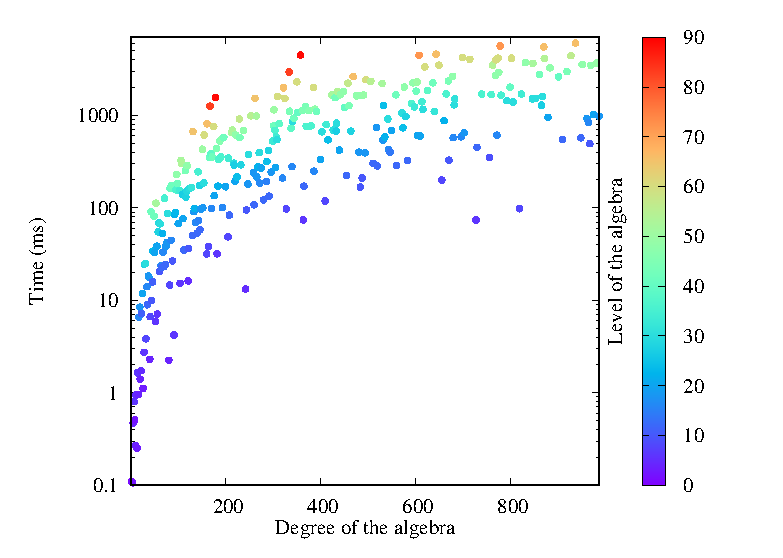
\includegraphics{benchmarks/lattice-h90/solve-h90-3.eps}
  \caption{Timings for computing decorated Kummer algebras $(A_m, \alpha_m)$ (logarithmic scale)
  with $p=3$.}
  \label{fig:solve-h90-3}
\end{figure}
\begin{figure}
  \centering
  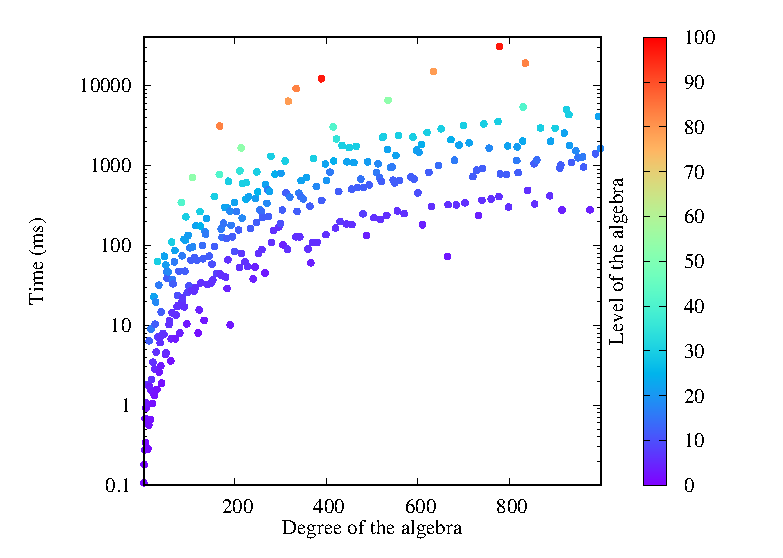
\includegraphics{benchmarks/lattice-h90/solve-h90-11.eps}
  \caption{Timings for computing decorated Kummer algebras $(A_m, \alpha_m)$ (logarithmic scale)
  with $p=11$.}
  \label{fig:solve-h90-11}
\end{figure}
In the complexity analysis of Proposition~\ref{prop:complexity-h90}, the level
of the algebra $A_m$ was bounded by its degree $m$, leading to a quasi-quadratic
complexity. However, we see in the timings that this bound is not relevant in
% TODO:
% =====
% Change that maybe? Not very smartly said. We could be more precise, and it is
% not even very true what we say...
practice. Indeed, the time results show that the level of the algebra has a
great impact on the timings: when the level is low, the computations are much
faster. In Figure~\ref{fig:level-12}, we selected only the computations that
occured on a fixed level $a=12$, and we see that in that case the time
complexity seems to be quasi-linear in the degree $m$.
\begin{figure}
  \centering
  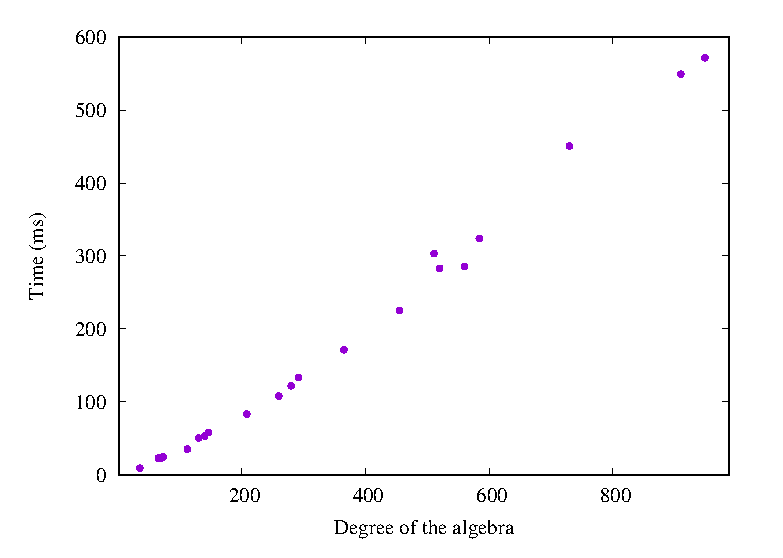
\includegraphics{benchmarks/lattice-h90/level-12.eps}
  \caption{Timings for computing decorated Kummer algebras $(A_m, \alpha_m)$ 
  with $p=3$ and with a given level $a=12$.}
  \label{fig:level-12}
\end{figure}
We also see that the characteristic $p$ has a small impact on the timings, as shown
in Figure~\ref{fig:degree-16} where we measure the timings for computing the
algebra $A_{16}$ and the corresponding solution of~\eqref{eq:h90-kummer}
$\alpha_{16}$, \ie we work with the fixed degree $m=16$ and we let the
characteristic be a prime number $p$ that grows from $3$ to $10^4$.
\begin{figure}
  \centering
  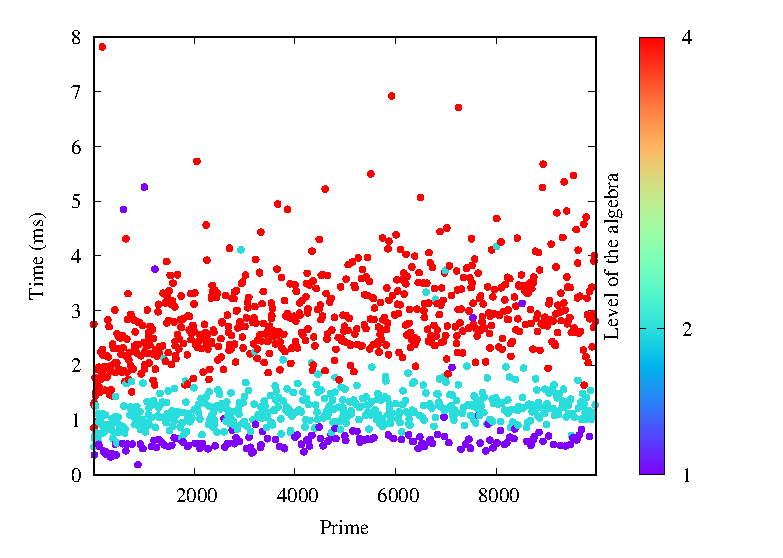
\includegraphics{benchmarks/lattice-h90/solve-h90-primes-degree-16.eps}
  \caption{Timings for computing decorated Kummer algebras $(A_{16},
  \alpha_{16})$ in characteristic $p$, with $p$ a prime number satisfying $3\leq
  p\leq 10^4$.}
  \label{fig:degree-16}
\end{figure}
The bottleneck of Algorithm~\ref{algo:decoration} appears to be the computation
of the $m$-th root extraction routine. When the decoration of two Kummer
algebras $A_m$ and $A_n$, with $m\mid n$, has been done; \ie when
Algorithm~\ref{algo:decoration} has been performed and solutions $\alpha_m$,
$\alpha_n$ are available, then the computation of the standard embedding
\[
  \mathbb{F}_{p^m}\emb\mathbb{F}_{p^n}
\]
is quite fast. In other words, Algorithm~\ref{algo:std-embed} is much faster
than Algorithm~\ref{algo:decoration}, which is a good thing because we only have
to call Algorithm~\ref{algo:decoration} once for each degree $m$, while
Algorithm~\ref{algo:std-embed} is called for each embedding computation, and
thus can be called several times with the same degree $m$. In
Figure~\ref{fig:embed-from-2}, we show the timings needed to compute embeddings
from $\mathbb{F}_{p^2}$ to $\mathbb{F}_{p^m}$, in the case where $p=3$, and for
every $4\leq m\leq 1000$ such that $p\nmid m$, $2\mid m$, and a suitable Conway
polynomial is available. Once again, the level of the destination algebra has an
important impact on the timings. 
\begin{figure}
  \centering
  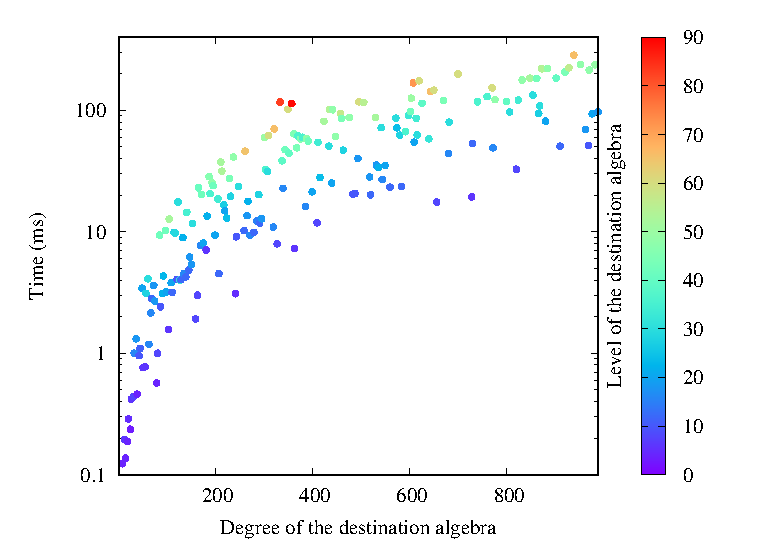
\includegraphics{benchmarks/lattice-h90/embed-from-degree-2.eps}
  \caption{Timings to compute the standard embedding from $\mathbb{F}_{p^2}$ to
  $\mathbb{F}_{p^m}$ (logarithmic scale), for $p=3$.}
  \label{fig:embed-from-2}
\end{figure}
We also measured the time needed to compute embeddings with extensions of a
fixed degree
\[
  \left[ \mathbb{F}_{p^{2m}}:\mathbb{F}_{p^m} \right] = 2
\]
in Figure~\ref{fig:embed-factor-2}, and we obtain similar results as in in
Figure~\ref{fig:embed-from-2} where the degree of the extension was varying but
the base field was fixed. Thus, it appears that the most important parameter
is the degree of the destination algebra.
\begin{figure}
  \centering
  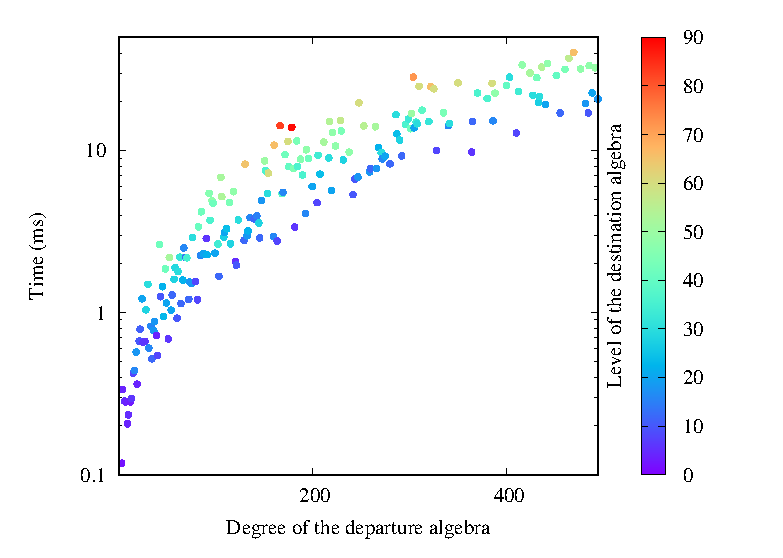
\includegraphics{benchmarks/lattice-h90/embed-factor-2.eps}
  \caption{Timings to compute the standard embedding from $\mathbb{F}_{p^m}$ to
  $\mathbb{F}_{p^{2m}}$ (logarithmic scale), for $p=3$.}
  \label{fig:embed-factor-2}
\end{figure}
Nevertheless, embedding computations seems to be faster with a small extension
degree. This is in particular shown in Figure~\ref{fig:embed-to-880}, where we
plot the timings for computing standard embeddings
\[
  \mathbb{F}_{p^d}\emb\mathbb{F}_{p^{880}}
\]
with $d\mid880$. The number $880$ was chosen because it is not divisible by
$p=3$ and because it has 20 different divisors, which is the maximum we can
obtain for numbers coprime to $3$ and less than $1000$. The number $560$ is
also suitable and produces similar results. We use logarithmic scale on the
abcissa axis because there is a greater number of small divisors.
\begin{figure}
  \centering
  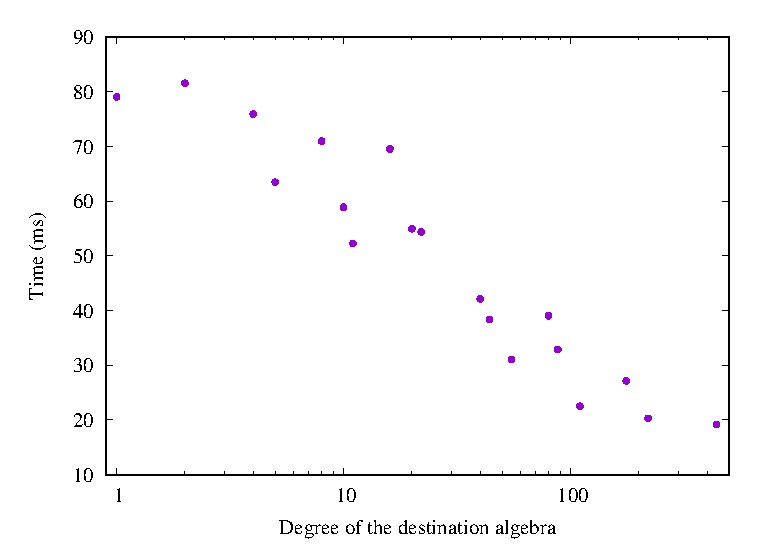
\includegraphics{benchmarks/lattice-h90/embed-to-degree-880.eps}
  \caption{Timings to compute the standard embedding from $\mathbb{F}_{p^d}$ to
  $\mathbb{F}_{p^{880}}$, for $p=3$ and $d\mid880$.}
  \label{fig:embed-to-880}
\end{figure}
The bottleneck of Algorithm~\ref{algo:std-embed} for computing a standard
embedding
\[
  \mathbb{F}_{p^m}\emb\mathbb{F}_{p^{n}}
\]
seems to be the powering $(\alpha_n)^{\frac{n}{m}}$ occuring in the destination algebra
$A_n$, which explains both the fact
that the algorithm is faster when the extension degree $\frac{n}{m}$ is smaller,
and the fact that the level of the destination algebra has an important impact
of the timings.
Again, we see in Figure~\ref{fig:embed-primes} that the impact of the
characteristic $p$ on the timings is minimal, compared to the other parameters.
\begin{figure}
  \centering
  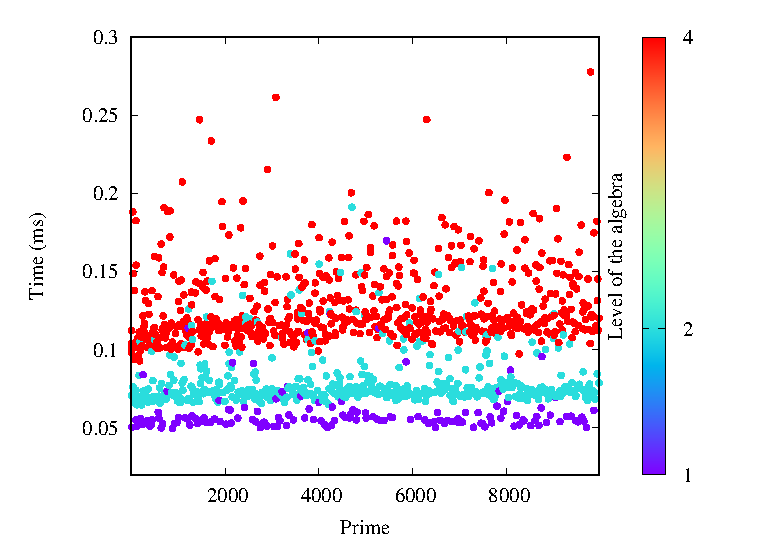
\includegraphics{benchmarks/lattice-h90/embed-primes-2-16.eps}
  \caption{Timings to compute the standard embedding from $\mathbb{F}_{p^2}$ to
  $\mathbb{F}_{p^{16}}$, for $p$ a prime number satisfying $3\leq p \leq 10^4$.}
  \label{fig:embed-primes}
\end{figure}

\section{Conclusion and perspectives}

In this chapter, we introduced a new idea to produce a lattice of compatibly
embedded finite fields, based on both Conway polynomials and Bosma-Canon-Steel
framework. Conway polynomials are used in many computer algebra systems, and
Bosma-Canon-Steel is used in Magma. Our idea exploits new techniques and is thus
interesting in itself. Furthermore, it also leads to a new family of (standard)
polynomials that can be used to define finite fields. Nevertheless, this new
family has no practical impact at the moment. Indeed, we can prove that
computing these polynomials is essentially equivalent to the computation of
Conway polynomials. Indeed, with our polynomials, one can recover a standard
solution $\alpha_m$ of~\eqref{eq:h90-kummer} and deduce the value
\[
  (\zeta_{p^a-1})^a.
\]
Then, by taking a $a$-th root, which is done in polynomial time in $m$, one can
find $\zeta_{p^a-1}$ and recover the associated Conway polynomial by computing a
minimal polynomial. This means that an efficient algorithm to compute our
standard polynomials would lead to an efficient algorithm to compute Conway
polynomials, which would be unexpected. We thus do not have great hope to find
such an algorithm, however the implemention presented in
Section~\ref{sec:implementation-std-lattices} is not the only possible way to
exploit our definitions. Indeed, it could be possible to loosen the assumption
that a cyclotomic lattice exists, and thus find a middle ground between the
rigidity of Conway polynomials and the flexibility of Bosma-Canon-Steel
framework, for example by lazily computing the roots of unity only when needed.
An orthogonal line of work would be to construct a complete lattice of
compatibly embedded finite fields, \ie working even with degrees that are not
coprime with the characteristic $p$ of the base field $\K$.
%


\clearpage
\bibliographystyle{alpha}
\bibliography{erou}

\end{document}
